\documentclass [11pt,twoside]{article}
\usepackage[shortlabels]{enumitem}
\usepackage{array}
\usepackage{hyperref}
\usepackage{multirow}
\usepackage{tabularray}
\usepackage[dvipsnames]{xcolor}
\usepackage{listings}
\renewcommand{\arraystretch}{1.3}
\usepackage[utf8]{inputenc}
\usepackage[T1]{fontenc}
\usepackage{enumitem}
\usepackage{svg}
%Page margins, header and footer positions
\usepackage{geometry}
\geometry{
 a4paper,
 total={210mm,297mm},
 left=25mm,
 right=25mm,
 top=30mm,
 bottom=25mm,
 headsep=7mm
}

\interfootnotelinepenalty=10000

%To display filling dots in the TOC for all entries
\usepackage[titles]{tocloft}
\renewcommand{\cftsecleader}{\cftdotfill{\cftdotsep}}

%Define new header and footer style
\usepackage{fancyhdr}

\pagestyle{fancy}
\fancyhf{}
\lhead{\color{Gray}{\small{DD by Akbulut \& Topcuoglu}}}
\lfoot{\textcolor{Gray}{\small{Copyright © 2023, Akbulut \& Topcuoglu – All rights reserved}}}
\rfoot{\textcolor{Gray}{\thepage}}
\renewcommand{\headrulewidth}{0pt}

%PACKAGES
\usepackage{wasysym}
\usepackage{pifont}

\newcommand{\supported}{\ding{52}\xspace}
\newcommand{\unsupported}{\ding{55}\xspace}
\newcommand{\partsupported}{\textcolor{black!40}{\ding{52}}\xspace}
\newcommand{\lowsupported}{\textcolor{black!20}{\ding{52}}\xspace}
\newcommand{\unknowsupported}{\textbf{?}\xspace}

%Font: Times
\usepackage{times}
%Change monospaced font
\renewcommand{\ttdefault}{lmtt}

%tables
\usepackage{tabu}
\usepackage{tabularx}
\usepackage{ltablex}
\usepackage{longtable}
\usepackage{float} % To allow the use of H modifier in long tables

%landscape mode
\usepackage{pdflscape}
\usepackage{rotating}
\usepackage{caption}

%make landscape mode be sensitive to even and odd pages
%start
\def\myrotate{\ifodd\c@page\else-\fi 90}
\makeatletter
\global\let\orig@begin@landscape=\landscape%
\global\let\orig@end@landscape=\endlandscape%
\gdef\@true{1}
\gdef\@false{0}
\gdef\landscape{%
    \global\let\within@landscape=\@true%
    \orig@begin@landscape%
}%
\gdef\endlandscape{%
    \orig@end@landscape%
    \global\let\within@landscape=\@false%
}%
\@ifpackageloaded{pdflscape}{%
    \gdef\pdf@landscape@rotate{\PLS@Rotate}%
}{
    \gdef\pdf@landscape@rotate#1{}%
}
\let\latex@outputpage\@outputpage
\def\@outputpage{
    \ifx\within@landscape\@true%
        \if@twoside%
            \ifodd\c@page%
                \gdef\LS@rot{\setbox\@outputbox\vbox{%
                    \pdf@landscape@rotate{-90}%
                    \hbox{\rotatebox{90}{\hbox{\rotatebox{180}{\box\@outputbox}}}}}%
                }%
            \else%
                \gdef\LS@rot{\setbox\@outputbox\vbox{%
                    \pdf@landscape@rotate{+90}%
                    \hbox{\rotatebox{90}{\hbox{\rotatebox{0}{\box\@outputbox}}}}}%
                }%
            \fi%
        \else%
            \gdef\LS@rot{\setbox\@outputbox\vbox{%
                \pdf@landscape@rotate{+90}%
                \hbox{\rotatebox{90}{\hbox{\rotatebox{0}{\box\@outputbox}}}}}%
            }%
        \fi%
    \fi%
    \latex@outputpage%
}
\makeatother
%end

%graphics
\usepackage{graphicx}
\usepackage[dvipsnames, table]{xcolor}
%If you upload images from PC, you need to insert code for the path here (different for Windows and Unix OS)

%References
%\usepackage{xpatch}
%\usepackage[backend=biber, style=numeric, citestyle=numeric, sorting=none]{biblatex}
%\addbibresource{main.bib}

%Other
\usepackage{ifthen}
\usepackage{xspace}
\usepackage{enumitem}
\usepackage{amssymb}
\usepackage[pdftex, colorlinks]{hyperref}
\newcommand{\comment}[1]{{\color{Red}$\blacktriangleright$ Comment: #1 $\blacktriangleleft$}}


% Some utilities\ldots
\usepackage{soul}
\usepackage{tikz}

\usetikzlibrary{calc}
\usetikzlibrary{decorations.pathmorphing}


\makeatletter

\newcommand{\defhighlighter}[3][]{%
  \tikzset{every highlighter/.style={color=#2, fill opacity=#3, #1}}%
}

\defhighlighter{yellow}{.5}

\newcommand{\highlight@DoHighlight}{
  \fill [ decoration = {random steps, amplitude=1pt, segment length=15pt}
        , outer sep = -15pt, inner sep = 0pt, decorate
       , every highlighter, this highlighter ]
        ($(begin highlight)+(0,8pt)$) rectangle ($(end highlight)+(0,-3pt)$) ;
}

\newcommand{\highlight@BeginHighlight}{
  \coordinate (begin highlight) at (0,0) ;
}

\newcommand{\highlight@EndHighlight}{
  \coordinate (end highlight) at (0,0) ;
}

\newdimen\highlight@previous
\newdimen\highlight@current

\DeclareRobustCommand*\highlight[1][]{%
  \tikzset{this highlighter/.style={#1}}%
  \SOUL@setup
  %
  \def\SOUL@preamble{%
    \begin{tikzpicture}[overlay, remember picture]
      \highlight@BeginHighlight
      \highlight@EndHighlight
    \end{tikzpicture}%
  }%
  %
  \def\SOUL@postamble{%
    \begin{tikzpicture}[overlay, remember picture]
      \highlight@EndHighlight
      \highlight@DoHighlight
    \end{tikzpicture}%
  }%
  %
  \def\SOUL@everyhyphen{%
    \discretionary{%
      \SOUL@setkern\SOUL@hyphkern
      \SOUL@sethyphenchar
      \tikz[overlay, remember picture] \highlight@EndHighlight ;%
    }{%
    }{%
      \SOUL@setkern\SOUL@charkern
    }%
  }%
  %
  \def\SOUL@everyexhyphen##1{%
    \SOUL@setkern\SOUL@hyphkern
    \hbox{##1}%
    \discretionary{%
      \tikz[overlay, remember picture] \highlight@EndHighlight ;%
    }{%
    }{%
      \SOUL@setkern\SOUL@charkern
    }%
  }%
  %
  \def\SOUL@everysyllable{%
    \begin{tikzpicture}[overlay, remember picture]
      \path let \p0 = (begin highlight), \p1 = (0,0) in \pgfextra
        \global\highlight@previous=\y0
        \global\highlight@current =\y1
      \endpgfextra (0,0) ;
      \ifdim\highlight@current < \highlight@previous
        \highlight@DoHighlight
        \highlight@BeginHighlight
      \fi
    \end{tikzpicture}%
    \the\SOUL@syllable
    \tikz[overlay, remember picture] \highlight@EndHighlight ;%
  }%
  \SOUL@
}

\makeatother

% Common abbrev. are set as commands to ensure proper spacing after the dot
\RequirePackage{xspace}
\newcommand{\ie}{i.e.\@\xspace}
\newcommand{\aka}{a.k.a.\@\xspace}
\newcommand{\Ie}{I.e.\@\xspace}
\newcommand{\cf}{cf.\@\xspace}
\newcommand{\Cf}{Cf.\@\xspace}
\newcommand{\eg}{e.g.\@\xspace}
\newcommand{\Eg}{E.g.\@\xspace}
\newcommand{\etal}{et al.\@\xspace}
\newcommand{\etc}{etc.\@\xspace}
\newcommand{\wrt}{w.r.t.\@\xspace}
\newcommand{\Wrt}{W.r.t.\@\xspace}



\date{}



\begin{document}

%TITLE PAGE

\begin{titlepage}


%LOGO

\begin{table}[t!]
\centering
\begin{tabu} to \textwidth { X[c] }

\includegraphics[scale=0.5]{Images/PolimiLogo} \\
\textbf{\small{Dipartimento di Elettronica, Informazione e Bioingegneria}} \\ 
\textbf{\small{Software Engineering 2}} \\
\end{tabu}
\end{table} ~
\\ [4cm]

%TITLE 

\begin{center}
    %Replace the text string with your title
{\textbf{\Huge{CodeKataBattle}}} \\ 
\vspace{2mm}
{\textbf{\small{Design Document}}} \\ 
{\textbf{\footnotesize{Version 1}}} \\ [4cm]
\textbf{\small{Mehmet Emre Akbulut}} \\
\vspace{1mm}
\textbf{\small{Yavuz Samet Topcuoglu}} \\ [1cm]
\textbf{\footnotesize{07 January 2024}}
\end{center}





\end{titlepage}

%Define deliverable specific info
%Replace cell contents where needed
\begin{table}[h!]
\begin{tabu} to \textwidth { X[0.3,r,p] X[0.7,l,p] }
\hline

\textbf{Deliverable:} & DD\\
\textbf{Title:} & CodeKataBattle - Design Document \\
\textbf{Authors:} & Mehmet Emre Akbulut, Yavuz Samet Topcuoglu \\
\textbf{Version:} & 1.0 \\ 
\textbf{Date:} & 07 January 2023 \\
\textbf{Download page:} & \href{https://github.com/mehmetemreakbulut/AkbulutTopcuoglu}{GitHub Repository} \\
\textbf{Copyright:} & Copyright © 2023, Akbulut \& Topcuoglu – All rights reserved \\
\hline
\end{tabu}
\end{table}




\setcounter{page}{2}


%------------------------------------------------------------------------------------------------------------------------------------------------
\newpage
\addcontentsline{toc}{section}{Table of Contents}
\tableofcontents
\newpage
\addcontentsline{toc}{section}{List of Figures}
\listoffigures
\addcontentsline{toc}{section}{List of Tables}
\listoftables

%------------------------------------------------------------------------------------------------------------------------------------------------
\clearpage
{\color{Blue}{\section{Introduction}}}
\label{sect:introduction}
\subsection{Purpose}
the CodeKataBattle project serves as a bridge between theoretical learning and practical application in computer science education. It offers students a platform to practice coding, collaborate, and improve their skills, and provides educators with effective teaching tools and assessment methods. The aim of CKB is to make computer science education more engaging, practical, and rewarding for both students and educators.

The goal of the \textbf{Design Document} is to provide a detailed explanation of the infrastructure utilized by the CodeKataBattle system. This includes a comprehensive description of the technologies and components employed, with a focus on the interactive actions of the system's users. The primary target audience for this document is developer teams who are responsible for implementing all the features.
\subsection{Scope}
The primary users of the platform are students and educators in the field of computer science and related areas.

\indent \textbf{CKB} is a web-based, interactive coding platform aimed at enhancing students' coding skills through battles created by educators. It serves primarily as an educational tool for practical application.CKB creates a competitive learning atmosphere where students are encouraged to excel in challenges formatted as battles, boosting their motivation.The platform fosters teamwork and collaboration, allowing students to work in groups on battles, mirroring real-world software development teamwork.

Educators have significant control over the platform, as they are responsible for creating, managing, and grading the battles and tournaments.

\indent \textbf{CKB} allows students to employ professional tools and methodologies, including version control and GitHub integration, to improve their real-world software development capabilities.
Automated testing is utilized by the platform for objective assessment of student submissions, while also enabling educators to conduct manual evaluations for more subjective aspects.

The platform is designed to provide immediate feedback on submissions and live updates on team scores and standings.

CKB offers educators flexibility in selecting programming languages, setting challenge difficulty, and determining the scope of coding tasks, catering to diverse educational requirements and learning paces.


\subsection{Definitions, Acronyms, Abbreviations}
\subsubsection{Definitions}
\begin{itemize}
    \item \textbf{Student}: An individual enrolled in an educational program or course who uses the platform to participate in coding exercises and improve software development skills.
    \item \textbf{Educator}: A person, such as a teacher or an instructor, responsible for creating coding challenges and managing learning activities on the platform.
    \item \textbf{Automated Testing}: A process where the CKB platform automatically executes predefined tests on student code submissions to assess their functionality and correctness without manual intervention.
    \item \textbf{Manual Scoring}: The process where educators evaluate student code submissions subjectively, complementing the automated testing system.
    \item \textbf{Battle}: A competitive coding challenge on the platform where students or teams of students solve specific programming problems within set parameters and time frames.
    \item \textbf{Tournament}: A series of code kata battles organized and managed by educators on the CKB platform, that ranks students or teams based on cumulative scores from individual battles.
    \item \textbf{Ranking}: A system within the CKB platform that orders participating students or teams based on their performance in individual code kata battles, determined by scores from automated and manual evaluations.
    \item \textbf{Leaderboard}: A feature on CKB that displays the standings of students or teams based on their performance overall in a tournament.
    \item \textbf{Institution Information}: Institution Information is multiple choice of institutions for the educators, a single institution for the students.
    \item \textbf{Unregistered User}: Users that haven't registered to the platform yet.
    \item \textbf{Registered User}: User that have registered to the platform.
    \item \textbf{Authenticated User}: User that have logged in to the platform.
    \item \textbf{Availability}: Availability is the status of tournament in terms of Closed, Open, or Upcoming.
    \item \textbf{Scoring Criteria}: Scoring Criteria includes Test Cases, Timeliness and Quality.
    \item \textbf{Quality Aspects:} Quality aspects are the concepts to score the submission in terms of quality. This term includes COMPLEXITY, DUPLICATIONS, MAINTAINABILITY, RELIABILITY, SECURITY, CLEAN\_CODE

\end{itemize}

\subsubsection{Acronyms}
\begin{itemize}
    \item \textbf{CKB}: CodeKataBattle
\end{itemize}

subsubsection{Abbreviations}
\begin{itemize}
    \item $AD_{x}$: x-th Activity Diagram
    \item $RW_{x}$: x-th Runtime View
    \item $UI_{x}$: x-th UI Design
    \item $R_{x}$: x-th Functional Requirement
\end{itemize}


\subsection{Revision History}
07-01-2024 : DDv1 \textbf{Final Version}

\subsection{Reference Documents}
\begin{itemize}
    \item Course Slides in WeBeep
    \item Project Assignment Document
    \item RASD CodeKataBattle
\end{itemize}
\subsection{Document Structure}

\begin{itemize}
    \item \textbf{Introduction:} This section provides an overview for the Design Document of CodeKataBattle,
    \item \textbf{Architectural Design:} In this section architectural views such as component view , deployment and runtime view are explained. Also components of the system and interfaces they provide are listed. Addition to architectural strategies, an high-level analysis of functionalities, responsibilities and the main components are explained.
    \item \textbf{User Interface Design:} The graphical respresentation of the system with respect to Design Document are shown here. Mockups are listed with respect to main functionalities of the system. In this section, we can see the system as whole from the user perspective.
    \item \textbf{Requirements Traceability:} This section contains mapping of functional requirements to the components, requirements and functionalites defined in the DD Document.
    \item \textbf{Implementation, Integration and Test Plan:} This section outlines the implementation of the system and the integration of its various application components. Additionally, it offers an in-depth explanation of how system testing is conducted.
    \item \textbf{Effort Spent:} The effort spent by group members are listed in terms of hours.
    \item \textbf{References:} The documents used, consulted and anaylzed are listed in this section.
\end{itemize}


%------------------------------------------------------------------------------------------------------------------------------------------------
\clearpage
{\color{Blue}{\section{Architectural Design}}}
\label{sect:architecture}
\subsection{Overview}
\indent The high-level architectural diagram provided below offers a conceptual overview of the CodeKataBattle (CKB) platform's infrastructure. It delineates the system's division into three primary layers: Presentation, Application, and Data. 
\newline
\indent The Presentation Layer captures the user interaction with the system via a standard web browser, illustrating the entry point for both educators and students. \\
\indent The Application Layer is the system's backbone, housing the business logic and core functionalities, including load balancing, application servers, and interfaces for external services such as the GitHub API, Static Analysis Tool API, Email Service, and Notification Service. A dedicated firewall protects this layer, ensuring secure data transactions. It is mainly responsible for handling requests from clients and presentation layer. This layer communicates with the Data Layer, to store and process the data.\\
\indent The Data Layer is structured to manage persistent data and comprises the Database Management System (DBMS), which supports sharded databases for scalability, and a File Storage system that accommodates various data types, including educator uploads and code submissions. This layer is mainly  responsible for data storage and access by querying. \\
\indent Each component is strategically placed to optimize performance and maintainability, reinforcing the platform’s robustness and reliability. The details are discussed in the following sections.
\newline
\indent Here, it is important to explain the reasons that led to choice of 3-Tier Architecture. Firstly, this kind of separation of logic helps to improve horizontal scalability. Each layer can be developed and maintained by different software teams. Also, different technologies can be adopted for presentation, application and data layers without affecting each other. \\
\indent On the other hand, another option can be Microservice Architecture, which is more modular then the 3-layered architecture.It provides higher degree of separation between each part of your application, which leads to even more flexibility and agility than you'd get from a three-tier app. However, as a trade-off, a Microservice Architecture includes more components to deploy and track, which makes developing and maintaining application more challenging because of the higher complexity. In this scenario, even orchestrators and service meshes can be needed. When we think about the CodeKataBattle platform specifically, the scalability of 3-layered architecture is well enough with several servers. A Microservice Architecture might not make sense when a large cluster which maximizes scalability and resilience is not used. Eventhough Microservice Architecture would be better option to scale up and down in a granular way, because of such complexity , it will be excessive for the CodeKataBattle. \\

\begin{figure}[H]
    \centering
    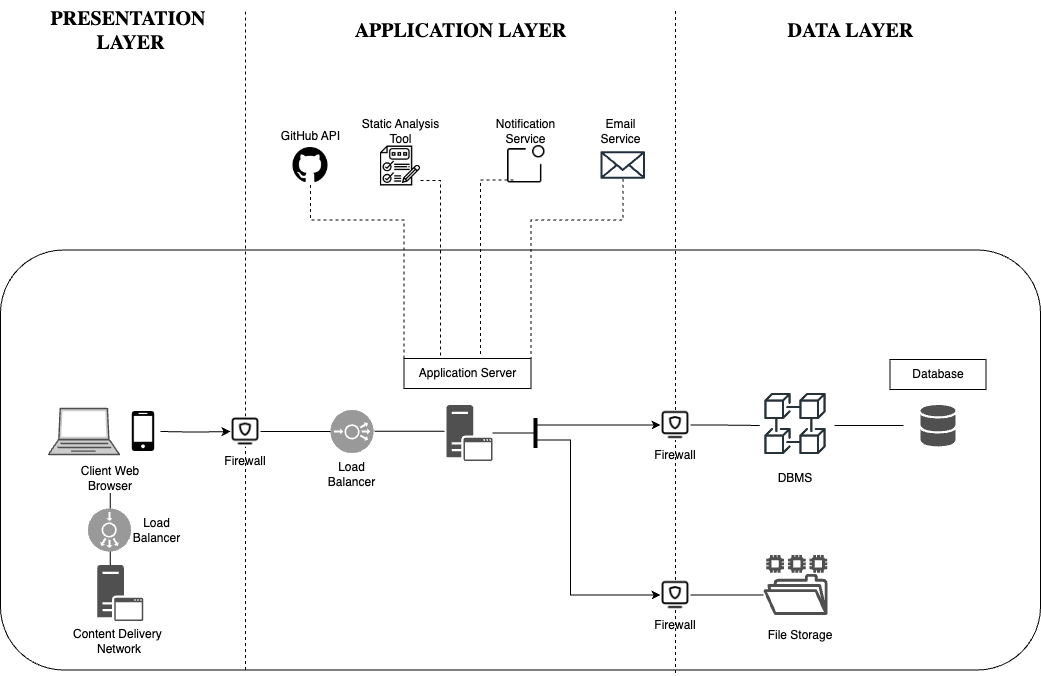
\includegraphics[scale=0.25]{Images/DD-highlevel-architecture.drawio.png}
    \caption{High-Level Architecture of the System}
\end{figure}

\newpage 
\subsection{Component View}

\begin{figure}[H]
    \centering
    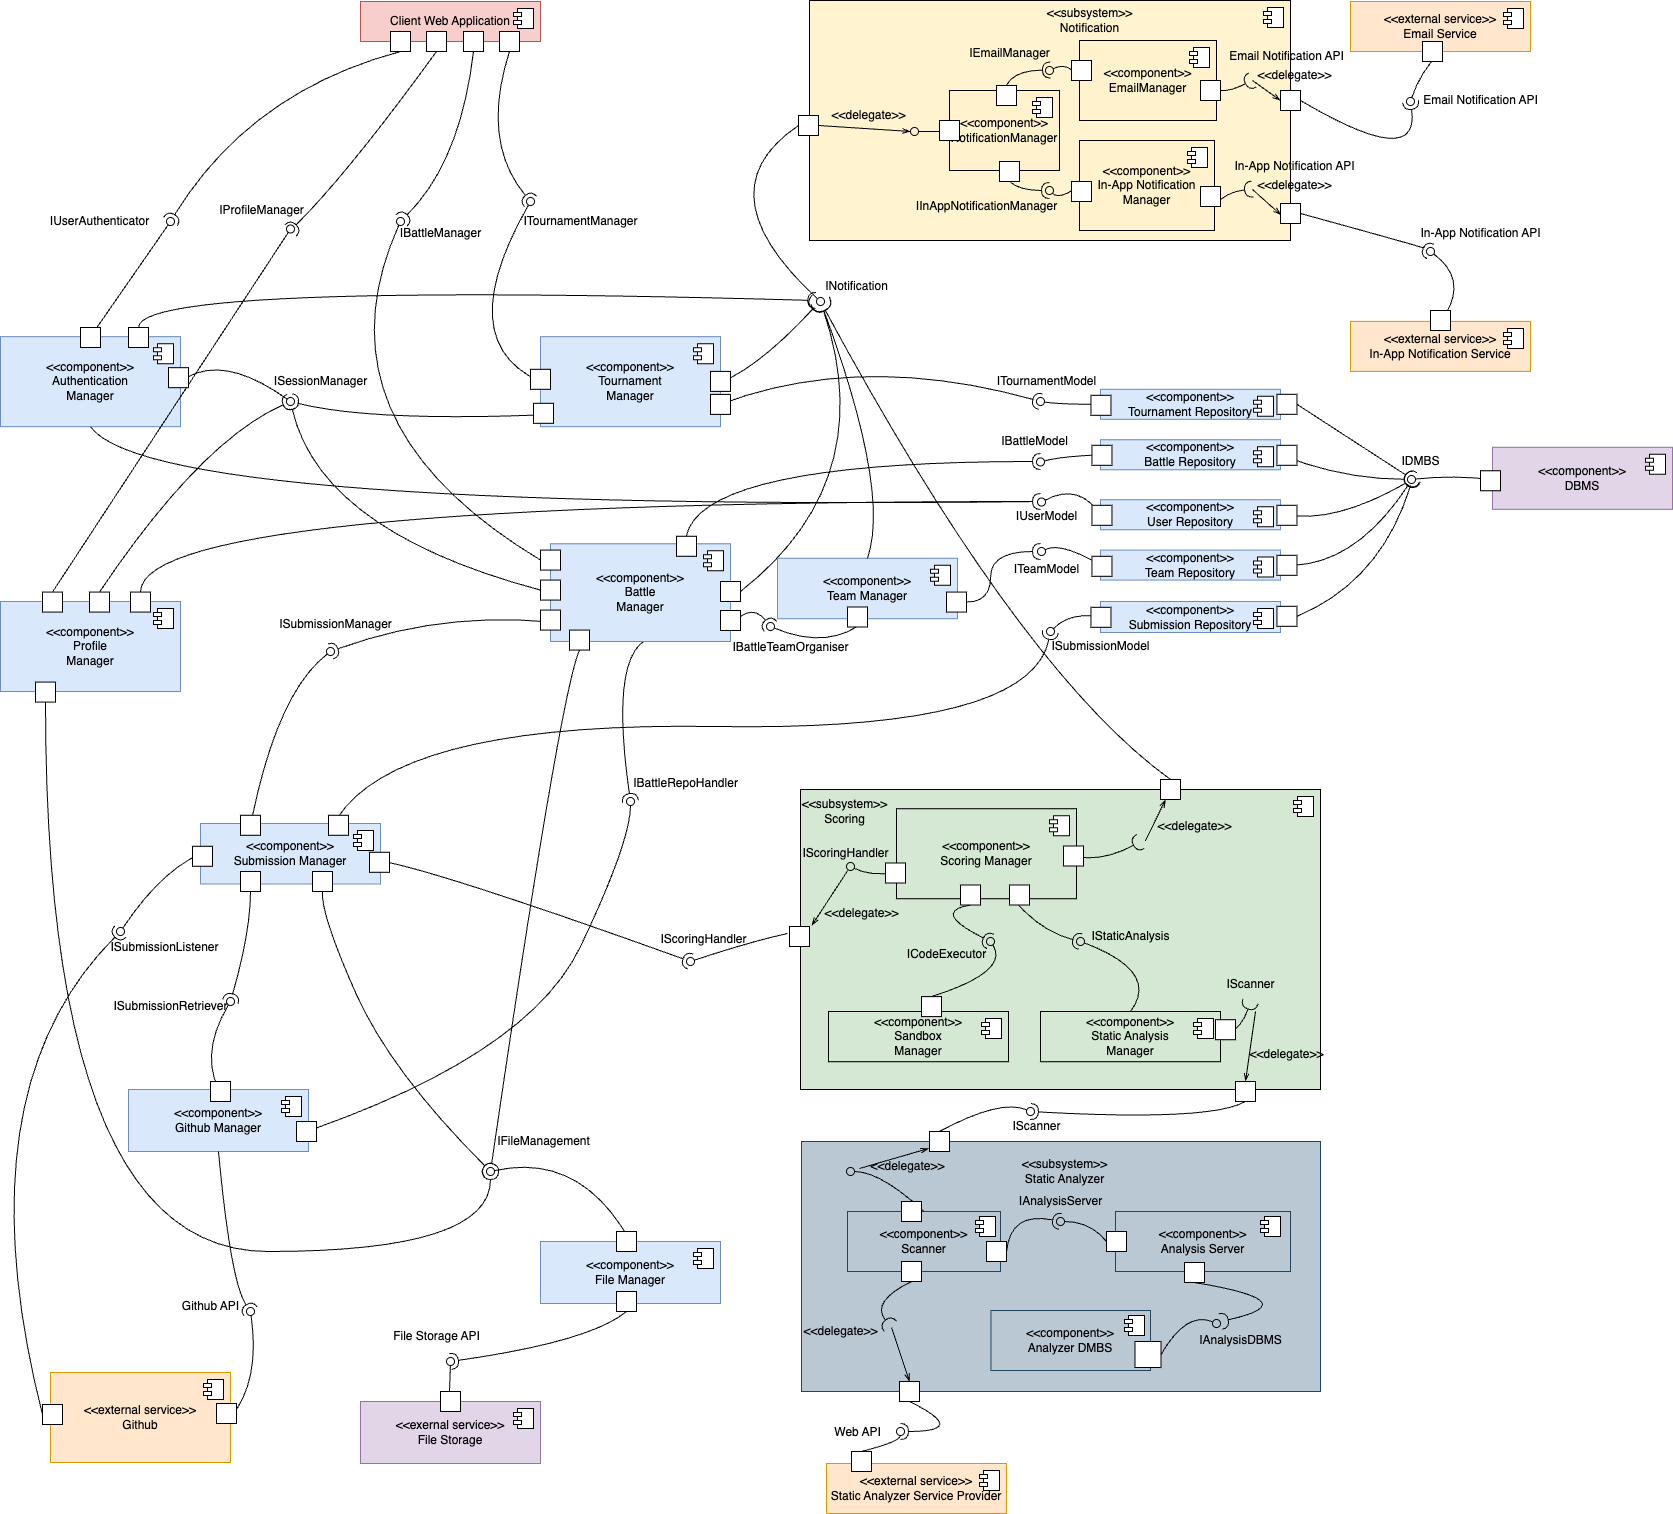
\includegraphics[width=\linewidth]{Images/DD-component.drawio.png}
    \caption{Component Diagram}
\end{figure}



\newpage
\subsection{Deployment View}
Our architecture mainly consists of 3 parts:  A Static Web Server, Application Server and Database Server.
\\
\indent Users can interact with website via a browser and a device that has browser support such as a computer, a mobile phone etc. Content Delivery Network is used for the web server which behaves as an entry point to users. It hosts the static and dynamic web content, such as .html, .css, .js, and image files, to users. Using Content Delivery Network has some advantages in terms of performance, reliability and security. CDNs speed up content delivery by decreasing the distance between where content is stored and where it needs to go, reducing file sizes to increase load speed, optimizing server infrastructure to respond to user requests more quickly. Also  if a server, a data center, or an entire region of data centers goes down, CDNs can still deliver content from other servers in the network. Moreover, it is also very useful from the security perspective. With their many servers, CDNs are better able to absorb large amounts of traffic, even unnatural traffic spikes from a DDoS attack, than a single origin server.
\\
\indent Then we have our Application Server which is hosted on the cloud with 2-4 instances. Also we have an additional Static Analysis Server.
\\
\indent At the Data Layer, we have database servers which includes database and DBMS with a firewall. 


\begin{figure}[H]
    \centering
    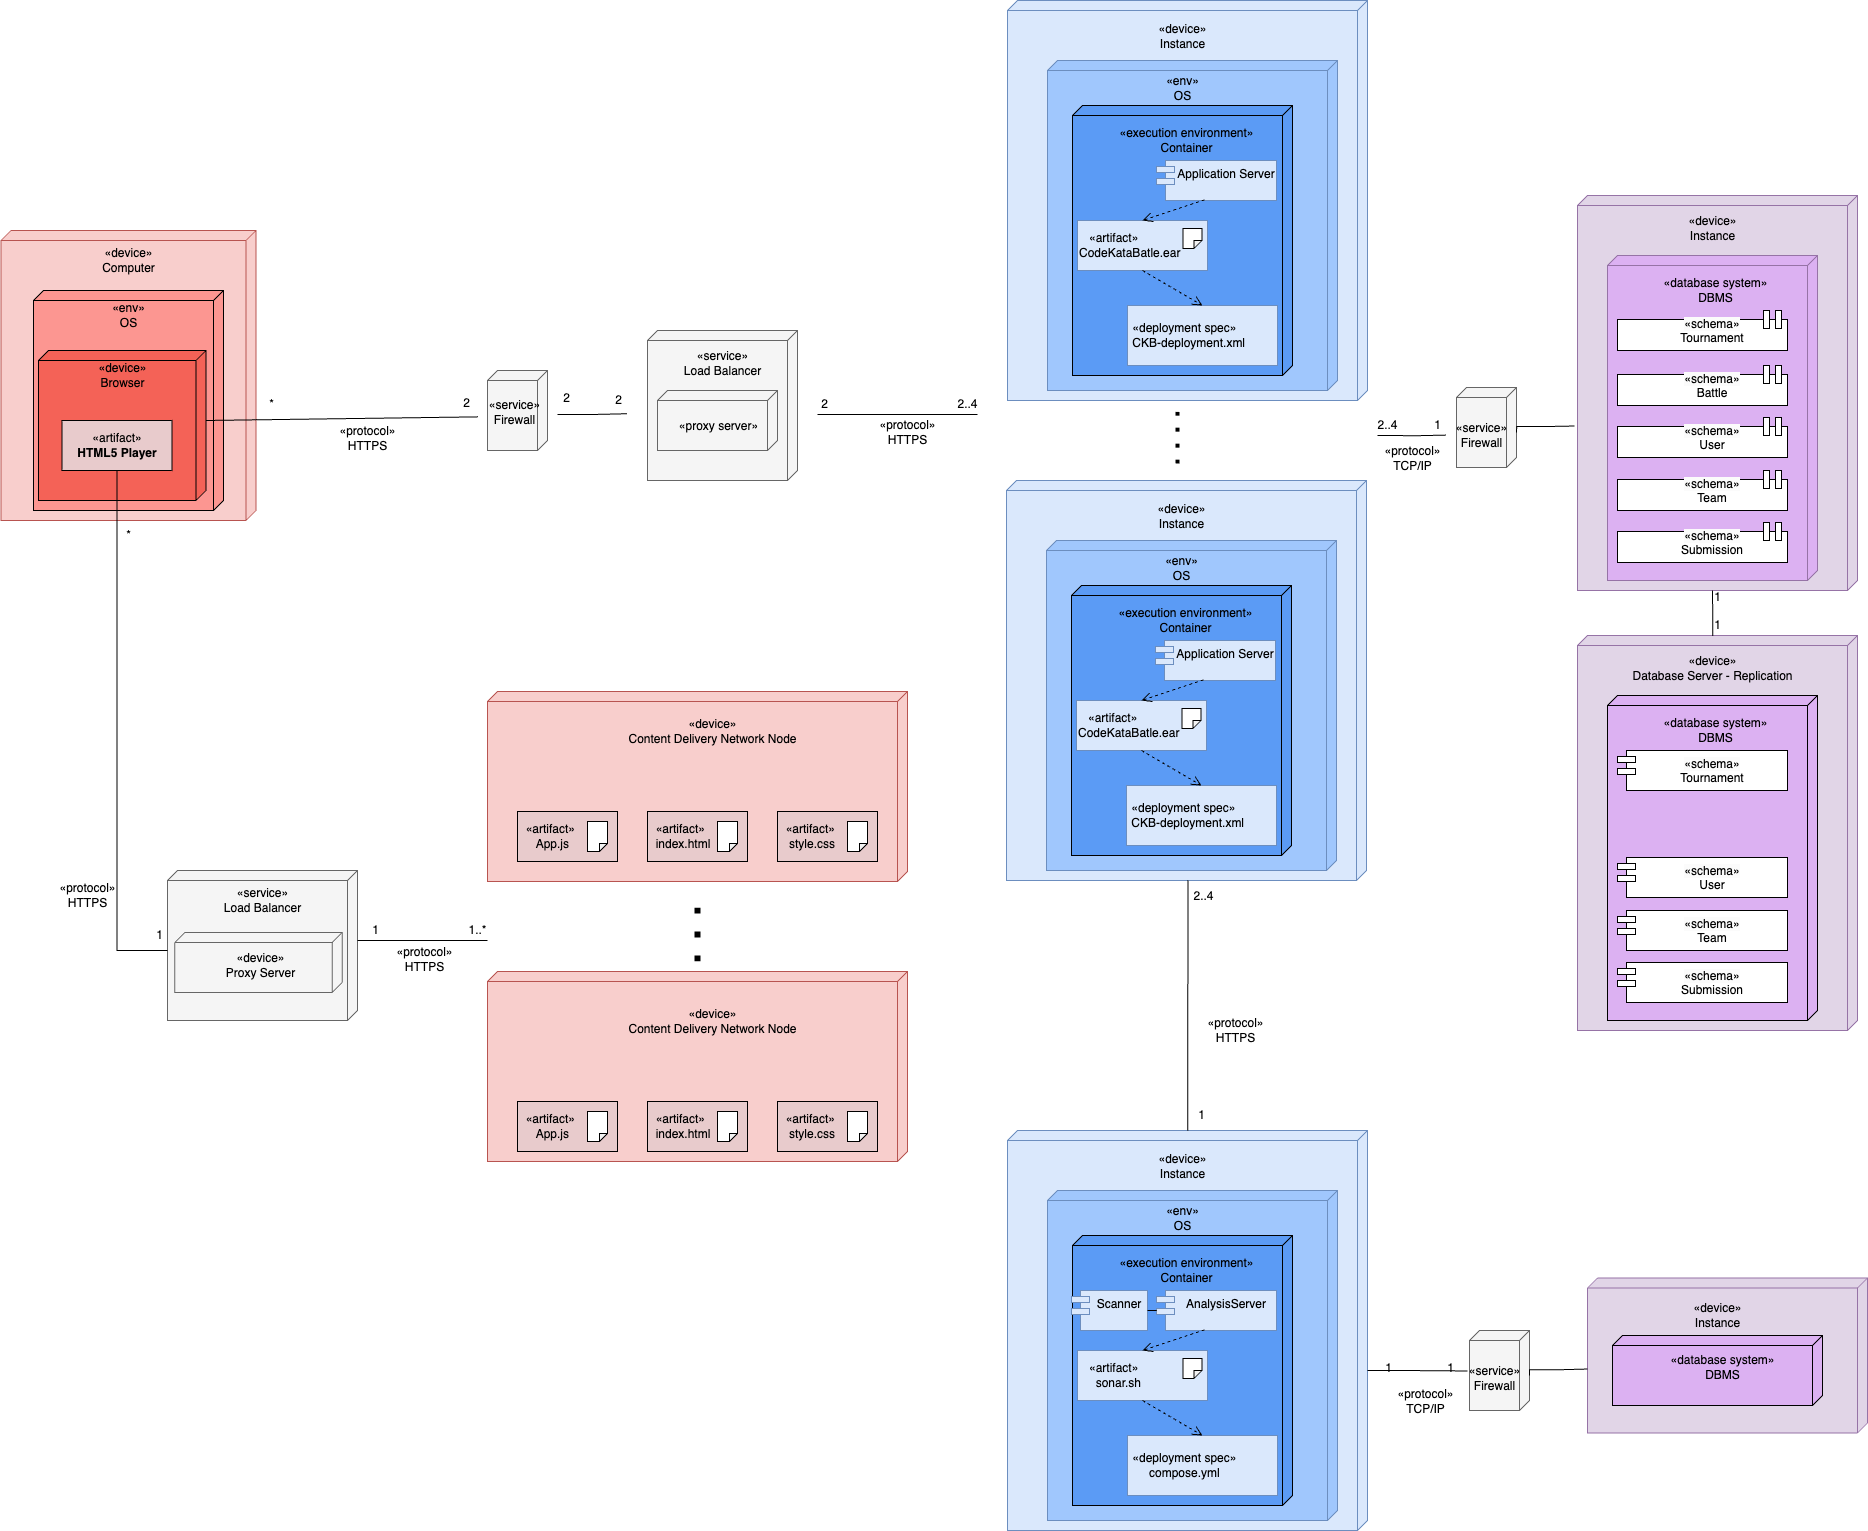
\includegraphics[scale=0.25]{Images/DD-deployment.drawio.png}
    \caption{Deployment Diagram}
\end{figure}

The deployment diagram offers a more detailed view over the hardware and software resources of the application:
\\
\indent \textbf{User Device:} User device can be any device that supports a web browser.
\\
\indent \textbf{Static Web Content:} The static web content of CodeKata Battle is hosted by Content Delivery Network with a Load Balancer distributing traffic and workload. The nodes in CDN can be scaled to very large numbers because it needs low computation power and memory. Geographically distributed nodes can be helpful to provide web interface with great performance in terms of speed. Briefly, The this content is static and all of its code is run on the
client’s machine,by browser, so there is no need for any logic to be implemented on the CDN side.
\\
\indent \textbf{Application Server:} All the business logic is handled in the Application Server which is hosted on the cloud with minimum 2 and maximum 4 instances. Obviously, these numbers can change in time but ,for an initial design, using 2-4 server instances would be adequate. Also 2 load balancer is used to distributing workload among application server instances. This is the bottleneck of the application so we decided to use 2 of them. 
\indent \textbf{Static Analysis Server:} Also, our static analysis solution requires a server that is responsible for static analysis. We conclude to add a server for this solution because most of the \textbf{Static Analysis Service Providers} works in that way. We followed the \textbf{SonarQube Documentation} as a solution  \hyperlink{https://docs.sonarsource.com/sonarqube/9.9/setup-and-upgrade/install-the-server/}{\textbf{Docs}}. We strongly suggest to use of this service. The internal components described in \textbf{Component View} can change if developers decide to implement a solution with another service.
\\
\indent Distributing incoming requests among multiple servers hosted on the cloud can helps us to fulfill some technical constraints:
\\
\indent \textbf{Reliability}: Cloud providers often offer high reliability through redundant resources and infrastructure. If one server fails, others can take over, minimizing downtime. Regular backups and disaster recovery options further enhance reliability.

\indent \textbf{Availability}: High availability is a key feature of these kind of hosting. Multiple instances in the cloud use multiple data centers around the world, ensuring that your services remain accessible even during local outages or disruptions.

\indent \textbf{Security}: Cloud providers invest heavily in security measures, including physical security of data centers, network security, and data encryption. Monitoring tools and firewall helps to sustain a secure application server.

\indent \textbf{Scalability}: Increasing or decreasing the size and amount of the instances can help to deal with changing request loads that servers have to respond to, also with the help of load balancing. Because of the changes in traffic or workload, we would need different computation and memory capacity. You can easily scale your server resources up or down based on demand, ensuring optimal performance without overpaying for unused capacity.

\indent \textbf{Maintainability}: Cloud providers handle hardware maintenance, updates, and patches, allowing us to focus on core business and application development. Also logging and monitoring tools generally works well with this kind of hosting other than in-house hosting or custom solutions we can develop.

\indent \textbf{Portability}: Cloud environments support portability and interoperability. You can move applications and data across different cloud environments or providers with relative ease, avoiding vendor lock-in and allowing for flexibility in deployment choices.
\\
\indent \textbf{Database}: This instance contains database with necessary schemas and database managements system. It is used with a replication It is also has a replicated version of itself, because of our \textbf{reliability} and \textbf{availability} constraints. By replicating data across multiple nodes or locations, the system can ensure high \textbf{availability}. If one node fails, the others can continue to operate, minimizing downtime and ensuring continuous access to data. Also, in the event of a major failure or disaster affecting the primary data center, having replicas ensures that data is not lost and can be quickly recovered. Also our static analysis solution requires a database instance for analysis server which is independent from other database instances.
\\
\indent \textbf{Firewalls:} Firewall services act as a security gatekeeper for a system's business and data layers, screening incoming connections. They enhance security by enforcing rules that either permit or block traffic, safeguarding the system from illicit access or harmful attacks.

\indent \textbf{Load Balancers:} A load balancer is employed to evenly distribute incoming traffic across various instances of an application. This strategy optimizes the use of resources, boosts performance, and maintains high availability. By doing so, the load balancer aids in managing a significant influx of requests, preventing the application from being overwhelmed or suffering downtime, and contributes to overall stability.


\newpage
\subsection{Runtime View}
This section includes the interaction of components for the important functionalities of the system. 
\subsubsection{User Registration}
Firstly, user sends the registration form from the registration screen. The pages differs for students and educators (see $UI_{1}$). Then system check that if this email exists or not. If it does not exis, the system creates user and send verification to user email. After verification, user registration process is completed successfully.
\begin{figure}[H]
    \centering
    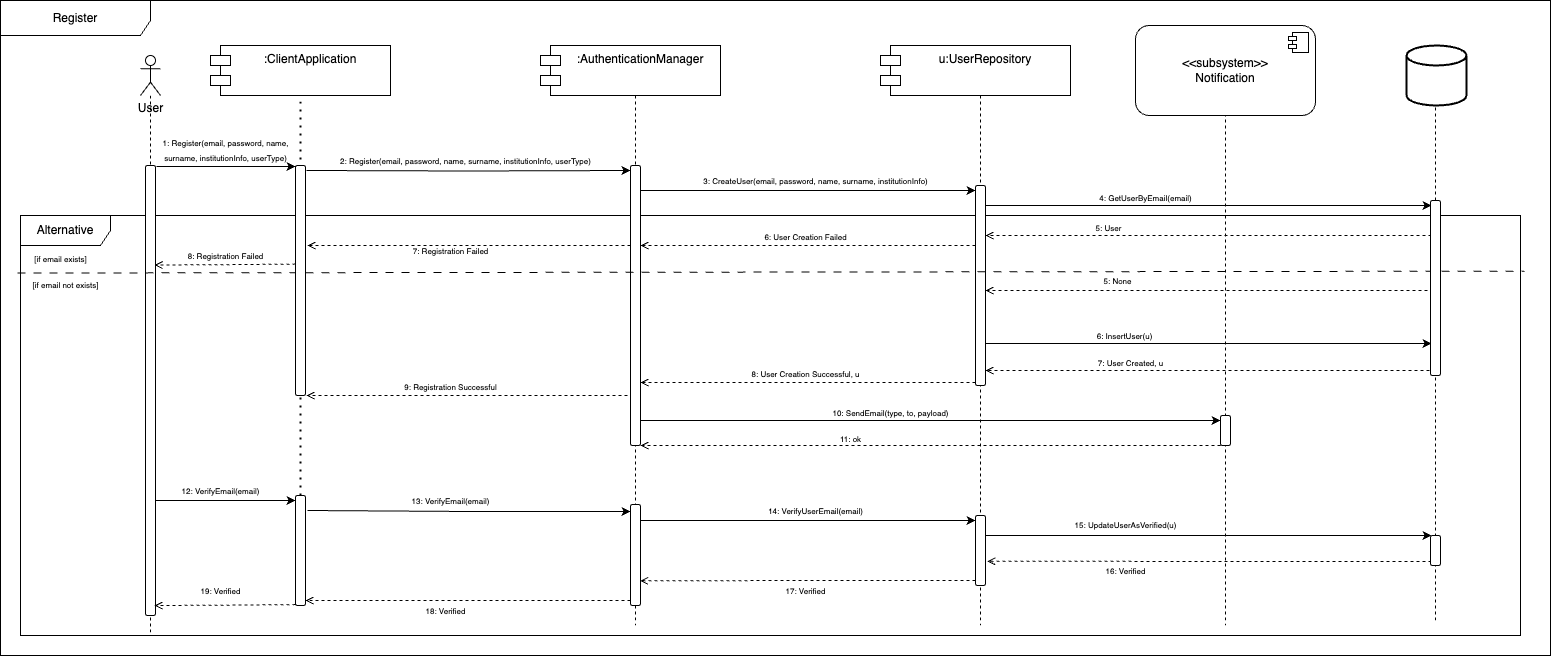
\includegraphics[width=\linewidth]{Images/runtime/register_runtime.drawio.png}
    \caption{$RW_{1}$} Registration
\end{figure}

\subsubsection{User Login}
Students and educators both need to login in order to use system functionalities. Only authenticated users can see the tournaments, battle etc. So user enters the credentials and system responds with respect to correctness of credentials.
\begin{figure}[H]
    \centering
    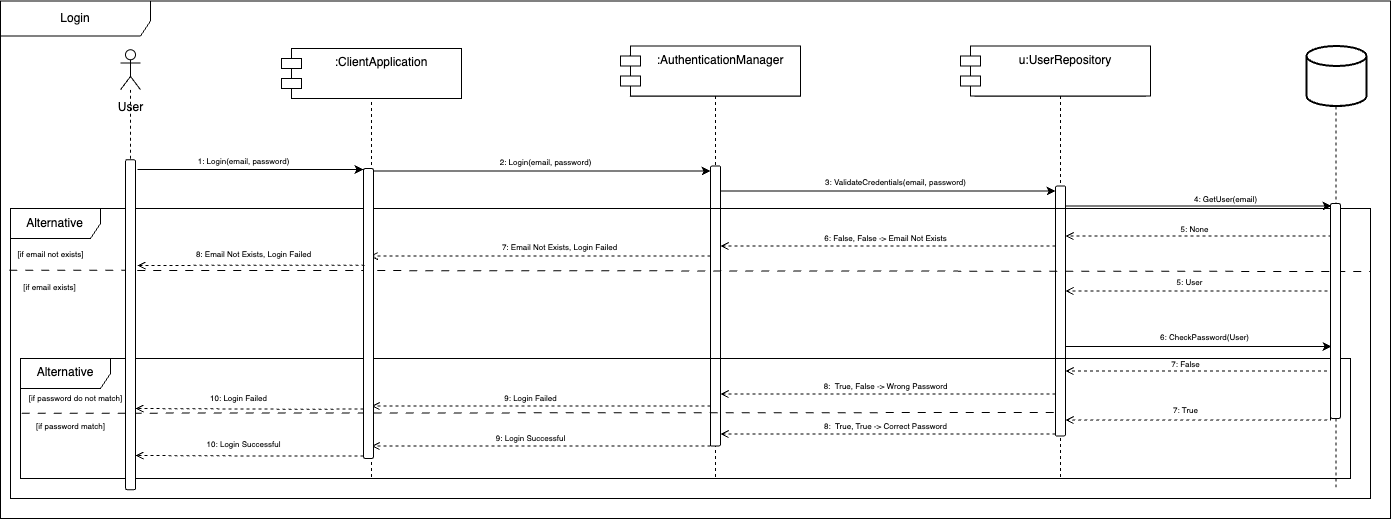
\includegraphics[width=\linewidth]{Images/runtime/login_runtime.drawio.png}
    \caption{$RW_{2}$} Login
\end{figure}

\subsubsection{View Tournament}
In this view some alternative ways to see the tournaments are shown. Fundamentally, students and educator can see all the tournaments. Also some options are available to filter the tournaments. After listing list of tournaments user can select and view on from them.
\begin{figure}[H]
    \centering
    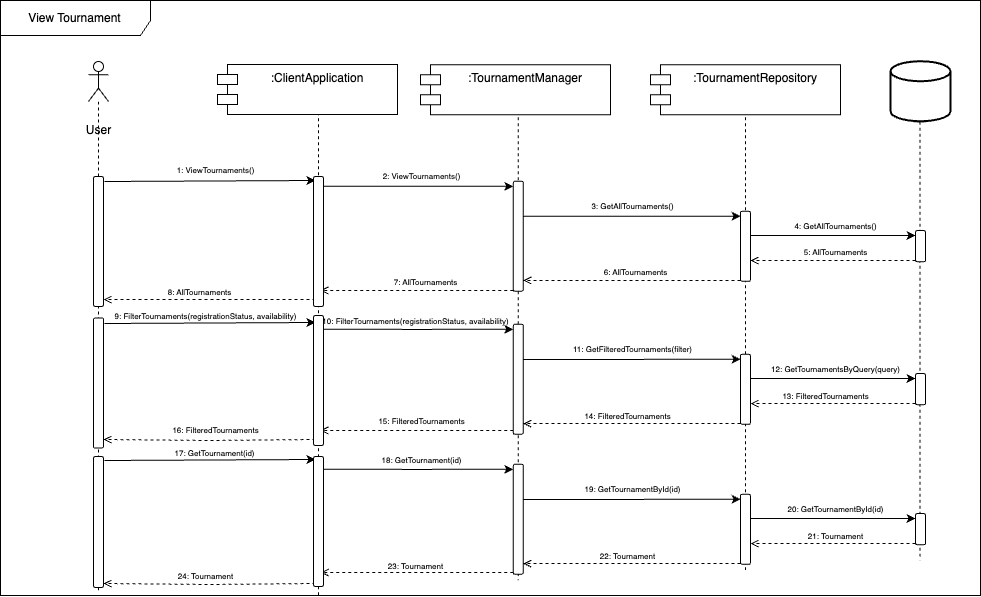
\includegraphics[width=\linewidth]{Images/runtime/view_tournament_runtime.drawio.png}
    \caption{$RW_{3}$} View Tournament
\end{figure}

\subsubsection{View Template}
This runtime view is a demonstration of all view functions of the application. Thanks to our layered approach, we can view the entities such as tournaments, battles, profiles. Consider this runtime view as a template.
\begin{figure}[H]
    \centering
    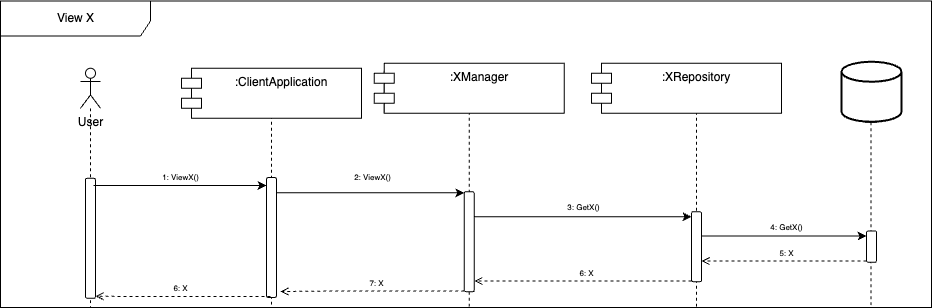
\includegraphics[width=\linewidth]{Images/runtime/view_template_runtime.drawio.png}
    \caption{$RW_{4}$} View Entity Template
\end{figure}

\subsubsection{Edit Profile}
This runtime view explains the sequences when a user want to edit their profiles. In the repository level there are functions for user type specific but this logic is encapsulated by Profile Manager, so endpoint is way simple.
\begin{figure}[H]
    \centering
    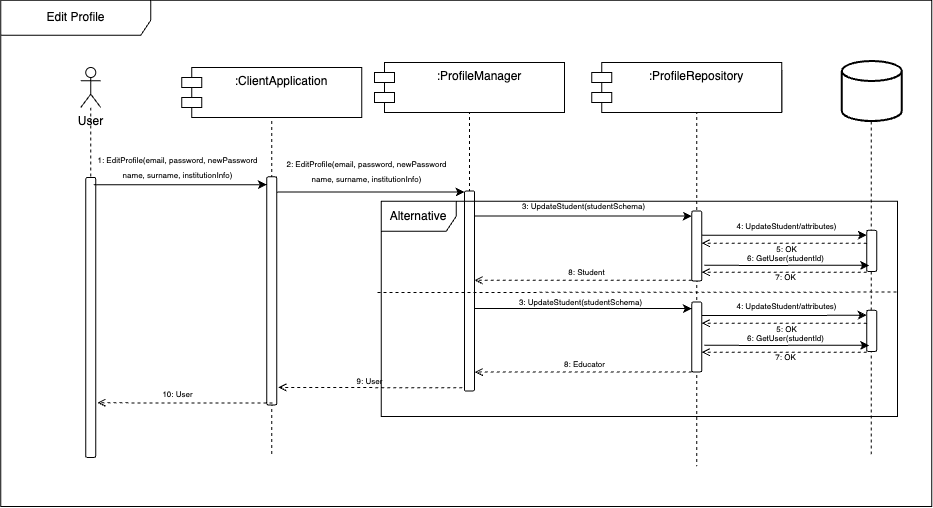
\includegraphics[width=\linewidth]{Images/runtime/edit_profile.drawio.png}
    \caption{$RW_{5}$} Edit Profile
\end{figure}


\subsubsection{Notification Subsystem}
Notification Subsystem is one of the core parts of the application. It consists of multiple components however other components of application sees only few function provided by Notification Manager. In this diagram we show a notification that send both email and in app notification. In other diagram we do not show all the process about notification, just show trigger function and response. This diagram explain what happens in a detailed way when a notification is sent .
\begin{figure}[H]
    \centering
    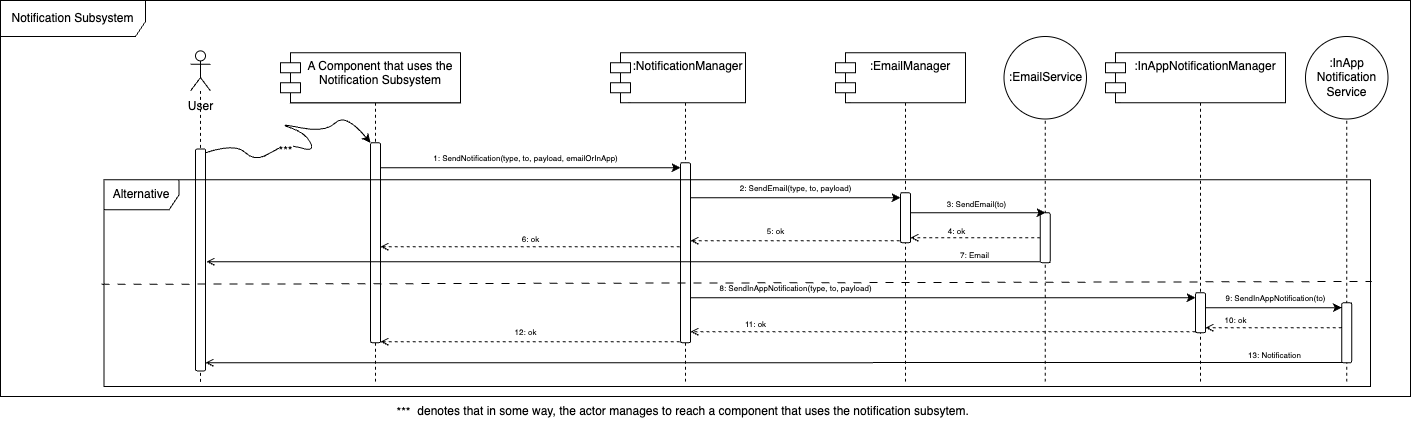
\includegraphics[width=\linewidth]{Images/runtime/notification_runtime.drawio.png}
    \caption{$RW_{6}$} Notification Subsystem
\end{figure}

\subsubsection{Session Management}
The main components that provides endpoints uses session information. They use the functions provided by ISesssionManager to retrieve user from the token provided in endpoint. 
\begin{figure}[H]
    \centering
    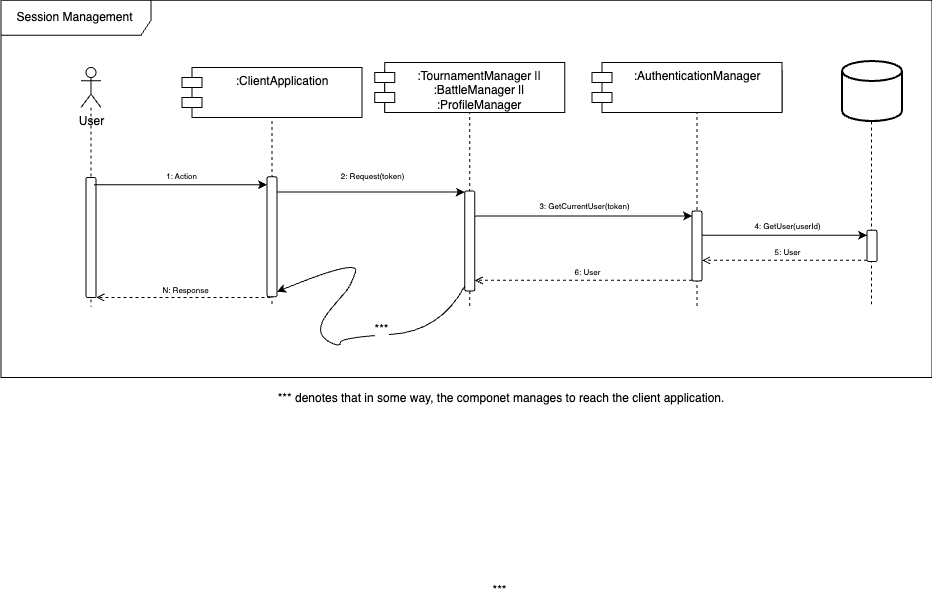
\includegraphics[width=\linewidth]{Images/runtime/session_runtime.drawio.png}
    \caption{$RW_{7}$} Session Management
\end{figure}


\subsubsection{Inspect Submission}
Educators can need to inspect a submission to view them or score manually.  This diagram explains the steps starting from battle to manual scoring. Of course manual scoring can be done if it is enabled in that battle.
\begin{figure}[H]
    \centering
    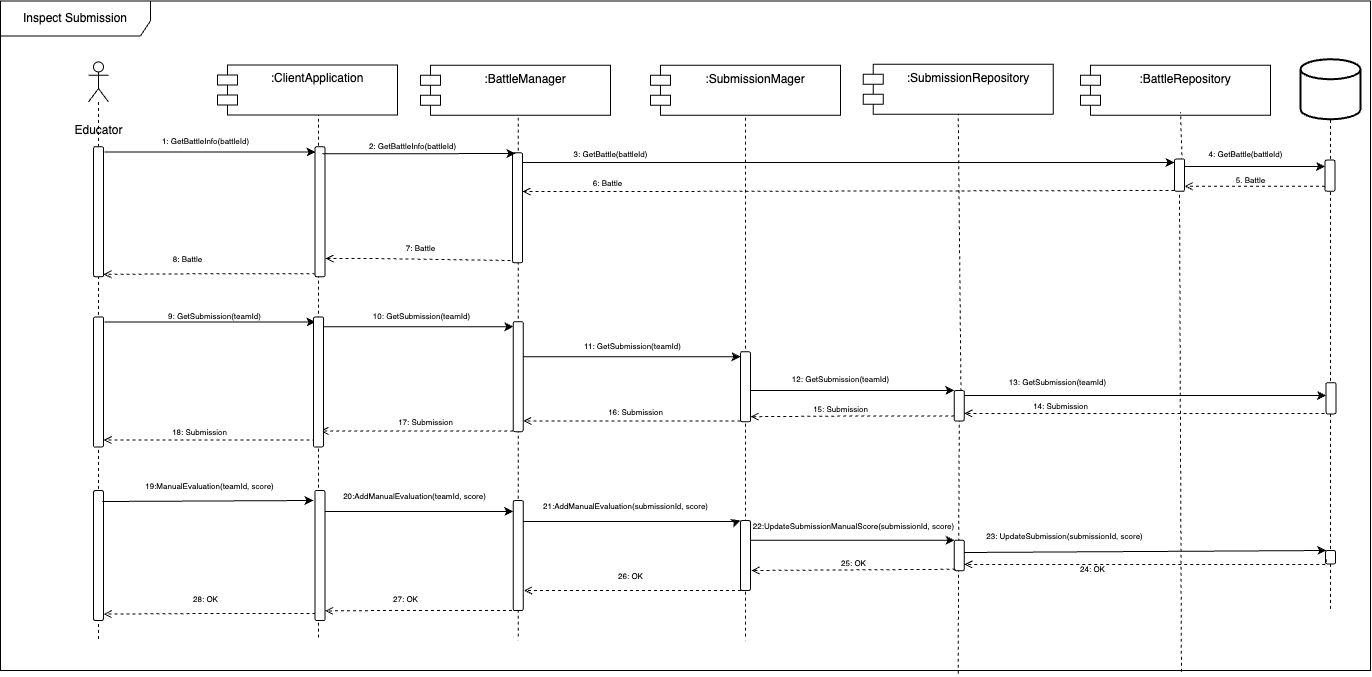
\includegraphics[width=\linewidth]{Images/runtime/inspect_submission_runtime.drawio.png}
    \caption{$RW_{8}$} Inspect Submission
\end{figure}


\subsubsection{Register To Tournament}
Students can register to Tournament. This diagram shows this process in a sequential way.
\begin{figure}[H]
    \centering
    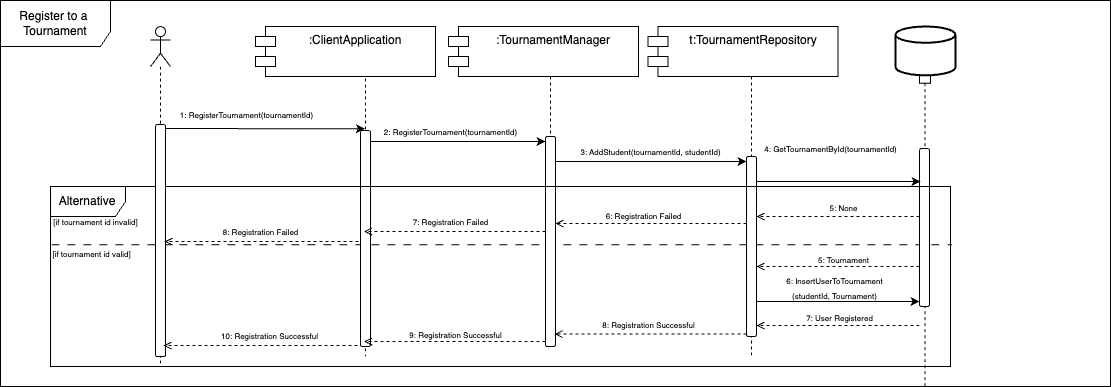
\includegraphics[width=\linewidth]{Images/runtime/register_tournament_runtime.drawio.png}
    \caption{$RW_{9}$} Register to Tournament
\end{figure}


\subsubsection{Register To Battle}
Students can register to Battle. This diagram shows this process in a sequential way.
\begin{figure}[H]
    \centering
    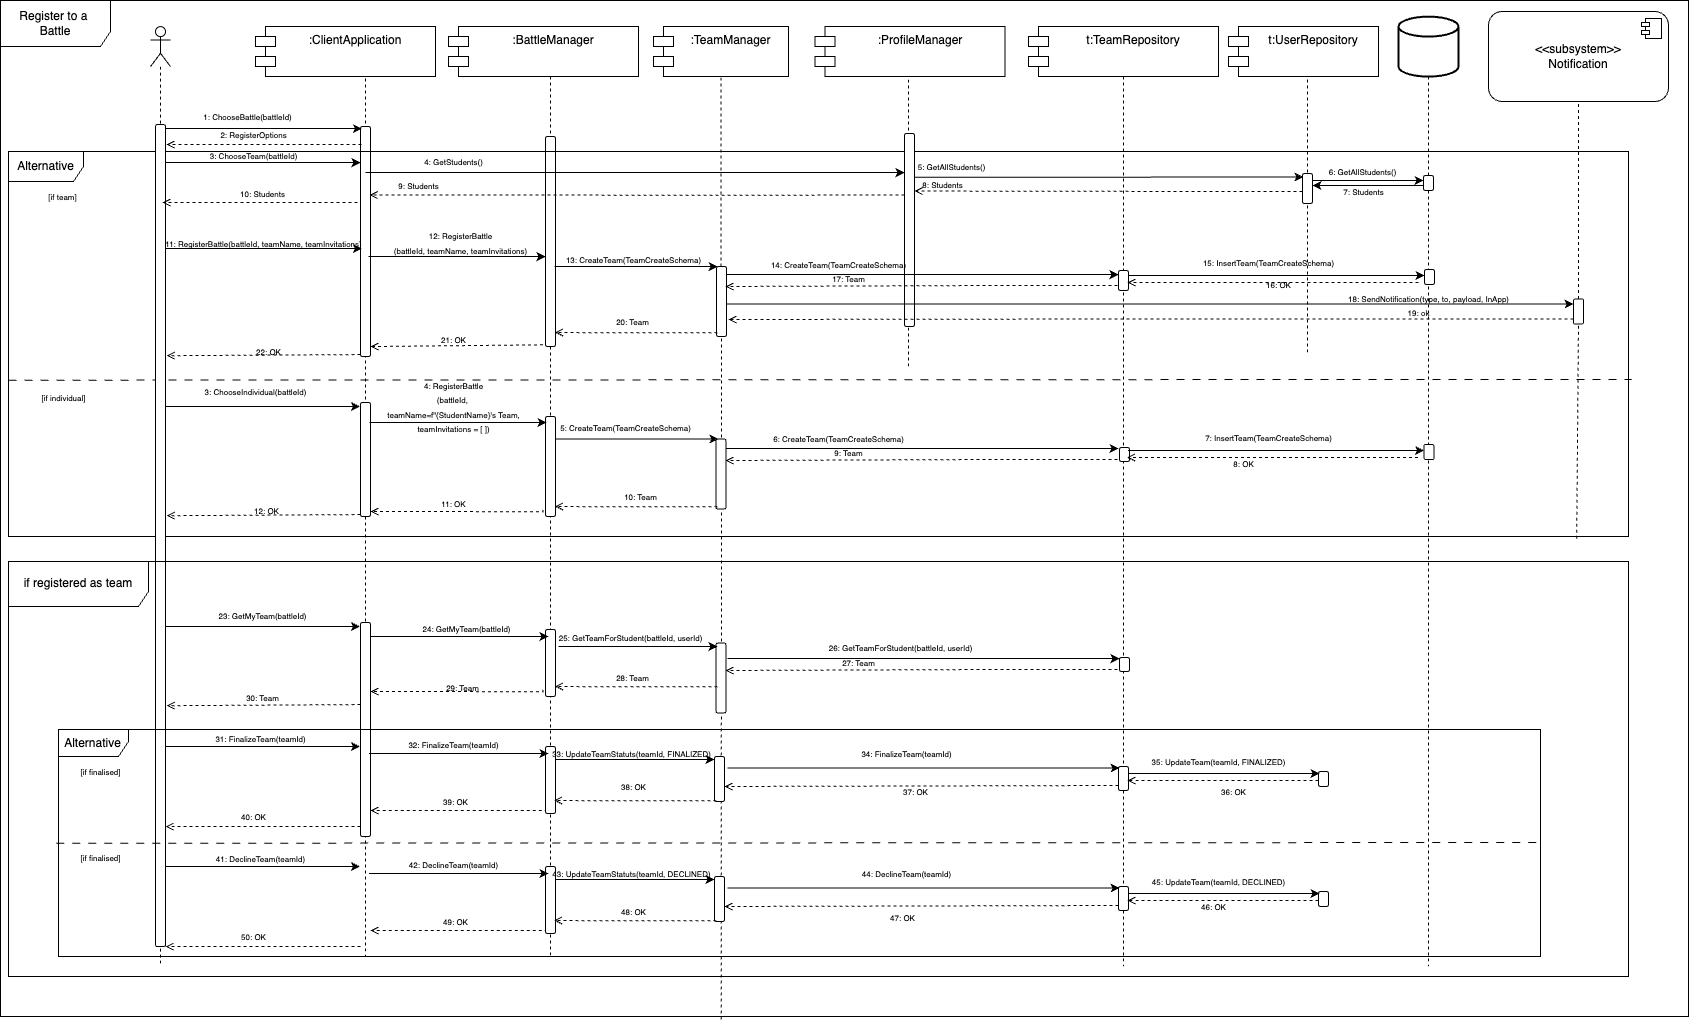
\includegraphics[width=\linewidth]{Images/runtime/register_battle_runtime.drawio.png}
    \caption{$RW_{10}$} Register to Battle
\end{figure}

\subsubsection{Create Tournament}
Educators can create tournaments. After tournament creation notifications are sent to all users.
\begin{figure}[H]
    \centering
    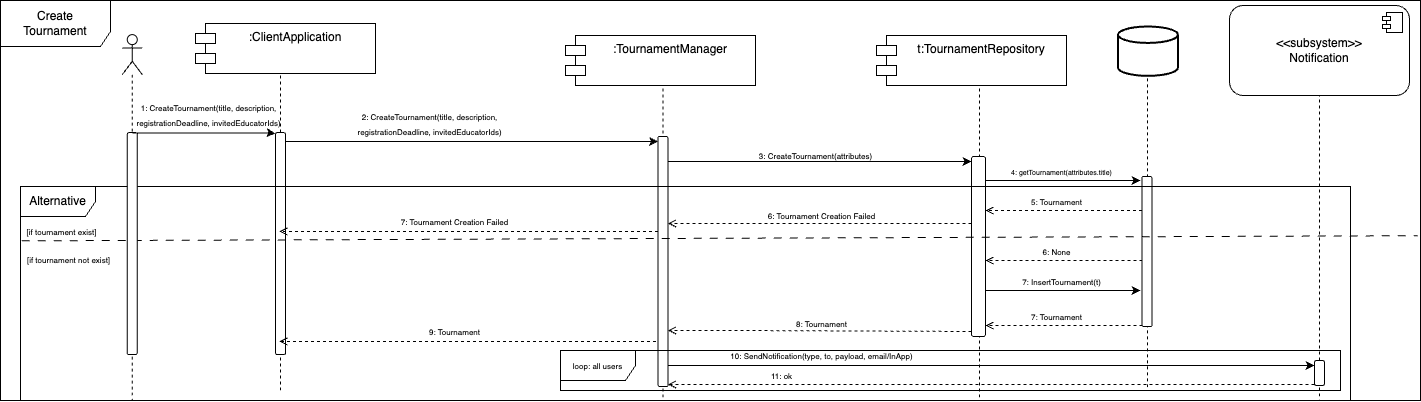
\includegraphics[width=\linewidth]{Images/runtime/create_tournament_runtime.drawio.png}
    \caption{$RW_{11}$} Create Tournament
\end{figure}

\subsubsection{Create Battle}
Educators can create battles. After battle creation notifications are sent to all users in tournament.
\begin{figure}[H]
    \centering
    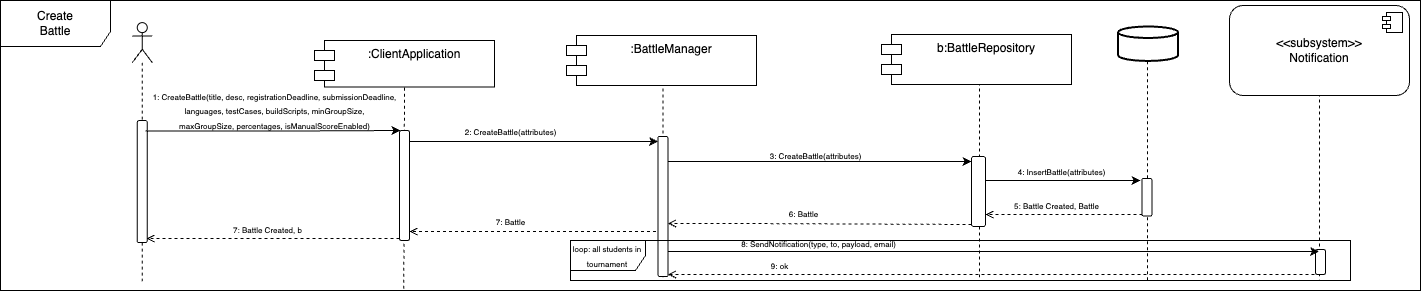
\includegraphics[width=\linewidth]{Images/runtime/create_battle_runtime.drawio.png}
    \caption{$RW_{12}$} Create Battle
\end{figure}

\subsubsection{Submission Handling}
This diagram shows the sequential actions when a submission occurs. Submission Handling is triggered by the Github commit from students.
\begin{figure}[H]
    \centering
    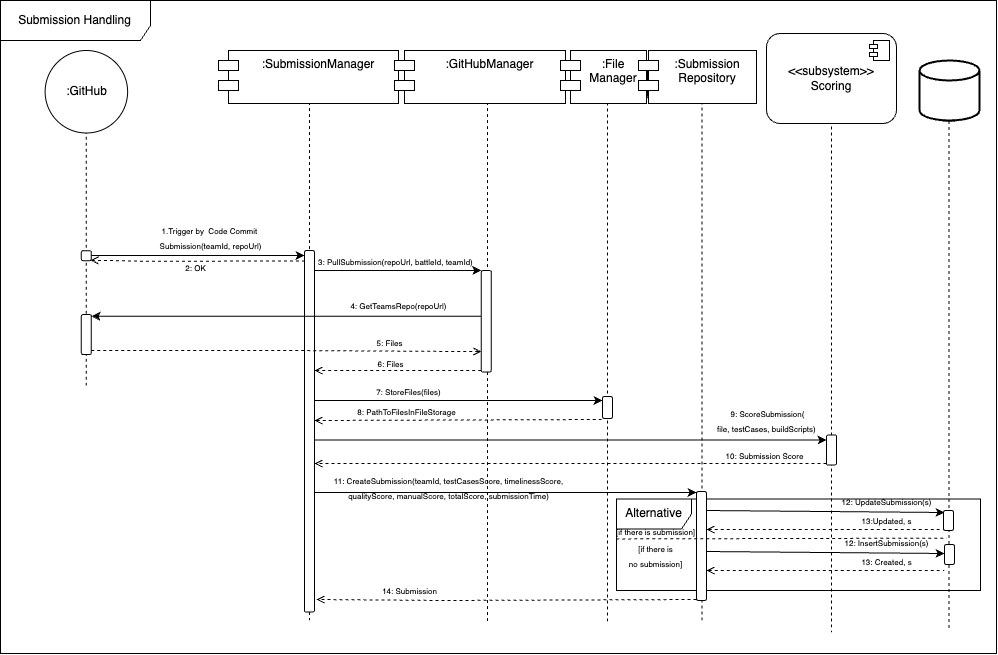
\includegraphics[width=\linewidth]{Images/runtime/submission_handling_runtime.drawio.png}
    \caption{$RW_{13}$} Submission Handling
\end{figure}



\subsubsection{Scoring Subsystem}
This diagram shows the sequential actions in scoring subsystem. Similar to notification subsystem, it has another components inside and only gives simple methods to other components in order to calculate scores.
\begin{figure}[H]
    \centering
    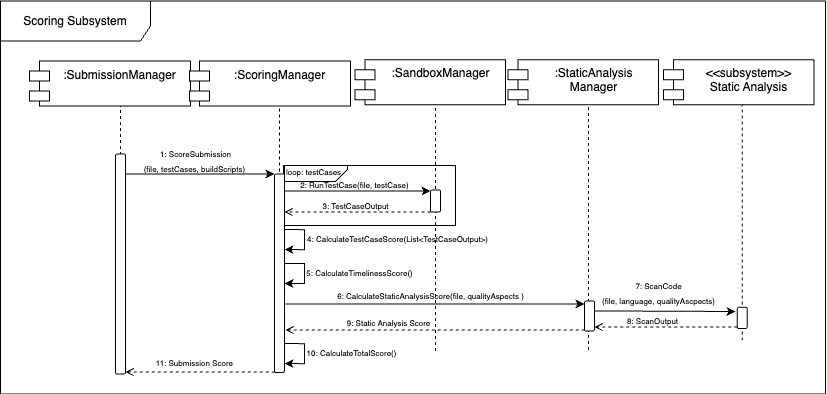
\includegraphics[width=\linewidth]{Images/runtime/scoring_subsystem_runtime.drawio.png}
    \caption{$RW_{14}$} Scoring Subsystem
\end{figure}



\subsubsection{Static Analysis Subsystem}
This diagram shows the sequential actions during static analysis. The Web API used by Scanner is not shown here because it is used for setup for authentication. Also API provides some endpoint to control server instead of CLI operations.
\begin{figure}[H]
    \centering
    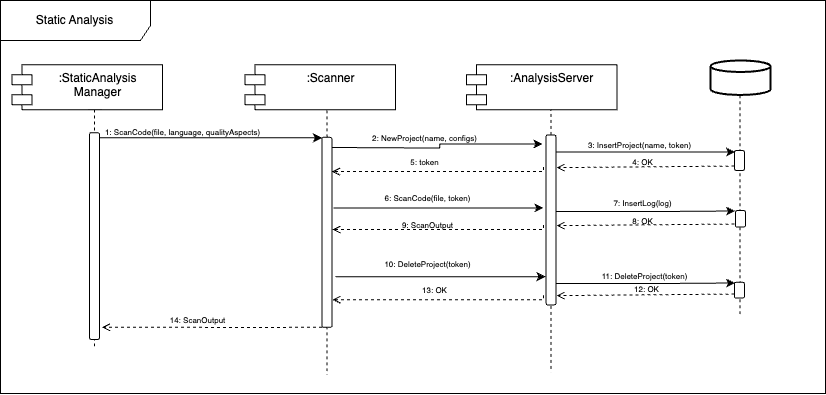
\includegraphics[width=\linewidth]{Images/runtime/static_analysis.drawio.png}
    \caption{$RW_{15}$} Static Analysis Subsystem
\end{figure}

\subsubsection{Battle Github Repository Creation}
After battle registration deadlines passed a Github repository must be created to be used by students. This diagram explains the Github repository creation of the battle.
\begin{figure}[H]
    \centering
    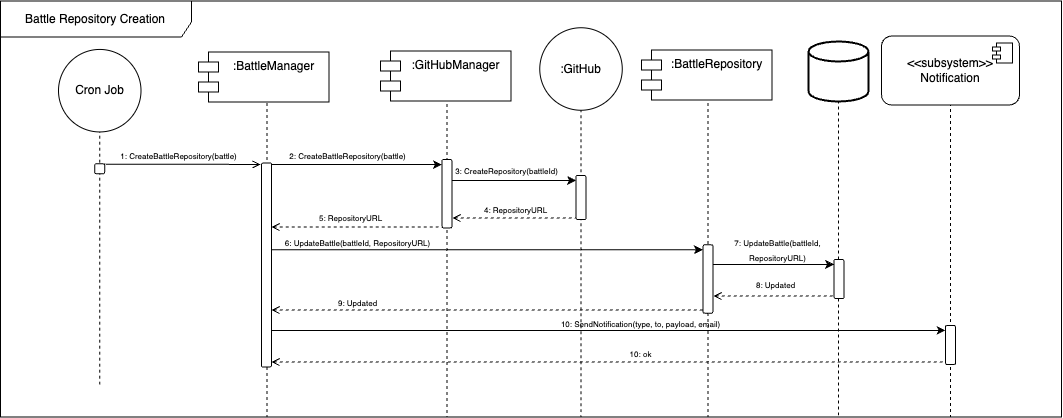
\includegraphics[width=\linewidth]{Images/runtime/battle_repository_runtime.drawio.png}
    \caption{$RW_{16}$} Battle Github Repository Creation
\end{figure}

\subsection{Component Interfaces}
In this section, we explain the interfaces and provided methods and returned objects. Also a class diagram is provided to show the dependencies and relations between the interfaces. Also at the end of the section endpoints provided by the system is listed and explained.

The Class Diagram is the same as Domain Level Class Diagram in RASD except some additional schmeas to demonstrate the data structures used in interfaces.
\begin{figure}[H]
    \centering
    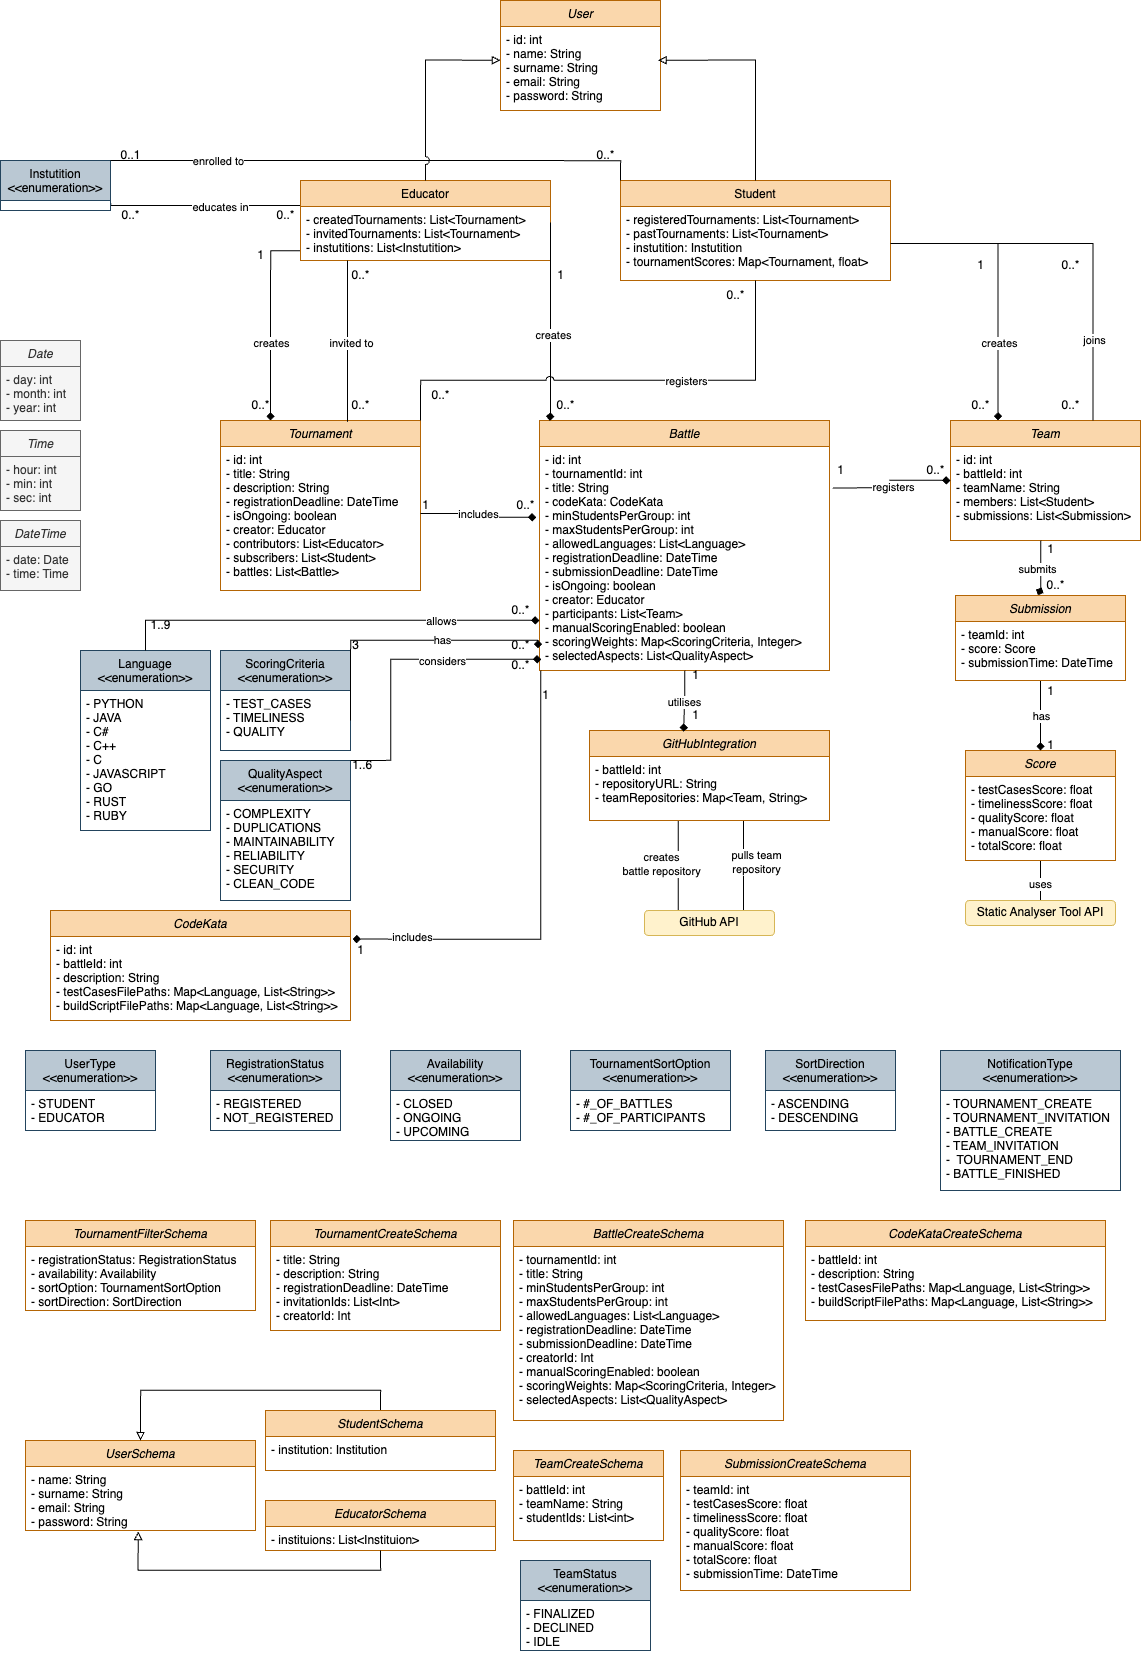
\includegraphics[width=\linewidth]{Images/DD-Class Diagram.drawio.png}
    \caption{Class Diagram (Based on RASD)}
\end{figure}

\subsubsection{IUserAuthenticator}
This Interface contains endpoints related to authentication of users. Endpoints explained in a detailed way at the end of the section. Just signatures are available here.
\begin{itemize}
\item Register(email: String, password: String, name: String, surname: String, institutionInfo: List<Institution>, userType: UserType) -> HTTP Response
\item Login(email: String, password: String) -> HTTP Response
\item Logout()-> HTTP Response
\item VerifyEmail(email:String) -> HTTP Response
\end{itemize}

\subsubsection{IProfileManager}
This Interface contains endpoints related to profiles of users. Endpoints explained in a detailed way at the end of the section. Just signatures are available here.
\begin{itemize}
\item GetMyProfile() -> HTTP Response
\item GetProfile(userId: int) -> HTTP Response
\item EditProfile(email: String, password: String, newPassword: String, name: String, surname: String, institutionInfo: List<Institution>) -> HTTP Response
\item GetEducators()-> HTTP Response
\item GetStudents()-> HTTP Response
\end{itemize}
\subsubsection{ITournamentManager}
This Interface contains endpoints related to Tournament. Endpoints explained in a detailed way at the end of the section. Just signatures are available here.
\begin{itemize}
\item GetTournaments(registrationStatus: RegistrationStatus, availability: Availability, sortOption: TournamentSortOption, sortDirection: SortDirection) -> HTTP Response
\item GetTournamentInfo(tournamentId: int) -> HTTP Status
\item RegisterTournament(tournamentId: int) -> HTTP Status
\item GetTournamentBattles(tournamentId: int, minGroupSize: int, maxGroupSize: int, startDate: DateTime, endDate: DateTime, registrationStatus: RegistrationStatus, institution: Institution, languages: List<Language>, educatorIds: List<int>, searchText: String) -> HTTP Response
\item GetTournamentLeaderboard(tournamentId: int) -> HTTP Response
\item ExportTournamentLeaderboard(tournamentId: int) -> HTTP Response
\item CreateTournament(title: String, description: String, registrationDeadline: DateTime, invitedEducatorIds: List<int>) -> HTTP Response
\item AnswerTournamentInvitation(tournamentId: int, isAccepted: boolean, educatorId: int) -> HTTP Response
\item EndTournament(tournamentId: int) -> HTTP Response
\end{itemize}

\subsubsection{IBattleManager}
This Interface contains endpoints related to Battle. Endpoints explained in a detailed way at the end of the section. Just signatures are available here.
\begin{itemize}
\item GetBattleInfo(battleId: int) -> HTTP Response
\item GetSubmission(teamId: int) -> HTTP Response
\item GetBattleRankings(battleId: int) -> HTTP Response
\item RegisterBattle(battleId: int, teamName: String, teamInvitations: List<int>) -> HTTP Response 
\item AnswerBattleInvitation(teamId: int, isAccepted: boolean, studentId: int) -> HTTP Response
\item FinalizeTeam(teamId: int) -> HTTP Response
\item DeclineTeam(teamId: int) -> HTTP Response
\item GetTeam(teamId: int) -> HTTP Response
\item GetMyTeam(battleId: int) -> HTTP Response
\item GetTeamScore(teamId: int) -> HTTP Response
\item AddManualEvaluation(teamId: int, score: float) -> HTTP Response
\item CreateBattle(title: String, description: String, registrationDeadline: DateTime, submissionDeadline: DateTime, languages: List<Language>, testCases: Map<String, List<File> >, buildScripts: Map<String, File>, minGroupSize: int, maxGroupSize: int, percentages: Map<String, int>, isManualScoreEnabled: boolean) -> HTTP Response 
\item ExportBattleLeaderboard(battleId: int) -> HTTP Response
\end{itemize}

\subsubsection{ISessionManager}
This Interface provides session related methods to components. Other components such as \textbf{Tournament Manager}, \textbf{Battle Manager} etc. They use to retrieve current user from token provided in request header in order to apply business logic related to specific user attributes.
\begin{itemize}
    \item getCurrentUser(token: String) -> User
\end{itemize}
\subsubsection{INotification}
This Interface provides methods that enables other components to send notifications via email or in-app notifications. \textbf{INotification} abstracts the internal operations related to using notification services and provides simple methods.

\begin{itemize}
    \item SendNotification(to: String, type: NotificationType, payload: Map<String,String>, emailOrInApp: ['EMAIL', 'NOTIFICATION']) -> boolean \\
    Calls methods below
    \item sendEmail(to: String, type: NotificationType, payload: Map<String,String>) -> boolean \\ This method sends email to given email with predefined email type related to a template and payload of it. Same method exists in \textbf{IEmailManager}.
    \item sendInAppNotification(userId: int, type: NotificationType, payload: Map<String,String>) -> boolean \\ This method sends in-app notification to given user id with predefined notification type related to a template and payload of it.Same method exists in \textbf{IInAppNotificationManager}.
\end{itemize}
\subsubsection{Repository Interfaces}
These interfaces are mainly responsible for the query management and communication with DBMS. They provide database query methods for other components. 
\begin{enumerate}
    \item \textbf{Tournament Repository}
    \begin{itemize}
        \item GetAllTournaments() -> List<Tournament> 
        \item GetFilteredTournament(filter: TournamentFilterSchema) -> List<Tournament>\\
        \item GetTournamentById(tournamentId: int) -> Tournament
        \item CreateTournament(attributes: TournamentCreateSchema) -> int (Tournament Id)
        \item EndTournament(tournamentId: int) -> boolean
        \item AddEducator(tournamentId: int, educatorId: int) -> boolean
        \item AddStudent(tournamentId: int, studentId: int) -> boolean
    \end{itemize}  
    \item \textbf{Battle Repository}
    \begin{itemize}
        \item GetBattle(battleId: int) -> Battle
        \item CreateBattle(attributes: BattleCreateSchema) -> Battle
        \item UpdateBattle(battleId: int, repoUrl: String) -> boolean
        \item CreateCodeKata(attributes: CodeKataCreateSchema) -> int (CodeKata Id)
    \end{itemize}
    \item \textbf{User Repository}
    \begin{itemize}
        \item CreateUser() -> User (This is a abstract method, use CreateStudent or CreateEducator)
        \item CreateStudent(attributes: StudentSchema) -> Student
        \item CreateEducator(attributes: EducatorSchema) -> Educator
        \item GetUser(userId: int) -> User
        \item GetAllStudents() -> List<User>
        \item GetAllEducators() -> List<User>
        \item UpdateStudent(attributes: StudentSchema) -> Student
        \item UpdateEducator(attributes: EducatorSchema) -> Educator
        \item DeleteUser(userId: int) -> boolean
        \item VerifyUserEmail(email:String) -> boolean
        \item ValidateCredentials(email: String, password: String) -> boolean, boolean
    \end{itemize}
    \item \textbf{Team Repository}
    \begin{itemize}
        \item CreateTeam(attributes: TeamCreateSchema) -> Team 
        \item FinalizeTeam(teamId: int) -> boolean
        \item DeclineTeam(teamId: int) -> boolean
        \item UpdateStudentStatus(teamId: int, studentId: int, isAccepted: boolean) -> boolean
        \item GetTeam(teamId: int) -> Team
        \item GetTeamForStudent(battleId: int, userId: int) -> Team
    \end{itemize}
    \item \textbf{Submission Repository}
    \begin{itemize}
        \item CreateSubmission(attributes: SubmissionCreateSchema) -> Submission \\
        This function overwrites the existing submission, more precisely, safe deletes it.
        \item GetSubmission(teamId: int) -> Submission
        \item GetSubmissions(battleId: int) -> List<Submission>
        \item UpdateSubmissionManualScore(submissionId: int, score: float) -> boolean
    \end{itemize}
\end{enumerate}
\subsubsection{IBattleTeamOrganiser}
\begin{itemize}
    \item UpdateTeamStatus(teamId: int, status: TeamStatus) -> boolean
    \item CreateTeam(attributes: TeamCreateSchema) -> Team
    \item GetTeam(teamId: int) -> Team
    \item GetTeamForStudent(battleId: int, studentId: int) -> Team
    \item AcceptTeamInvitation(teamId: int, studentId: int) -> boolean
    \item DeclineTeamInvitation(teamId: int, studentId: int) -> boolean
\end{itemize}
\subsubsection{ISubmissionManager}
\begin{enumerate}
    \item GetSubmission(teamId: int) -> Submission
    \item GetBattleScores(battle: Battle) -> List<Map<Team, int> >
   \item AddManualEvaluation(submissionId: int, score: float) -> boolean
\end{enumerate}
\subsubsection{ISubmissionListener}
\begin{enumerate}
    \item Submission(teamId: int, repoUrl: string) -> HTTP Status \\
    This is an endpoint responsible to be triggered by Github Actions Workflow created by teams. When they made a new commit, they  send a request to this endpoint.
\end{enumerate}
\subsubsection{ISubmissionRetriever}
\begin{enumerate}
    \item PullSubmission(repoUrl: String, battleId: int, teamId: int) -> String \\
    This method provides the url of a folder in the file storage system. The pulled repository content is stored in this folder with a naming using battleId and teamId. The component using this method is then responsible for other actions.
    \end{enumerate}
\subsubsection{IScoringHandler}
\begin{enumerate}
   \item ScoreSubmission(code: File, testCaseFiles: Map<Language, List<File> >, buildScripts: Map<Language, List<File> >) -> float
  \item CalculateTestCaseScore(List<TestCaseOutput>) -> float
   \item CalculateStaticAnalysisScore(code: File, qualityAspects: List<QualityAspect>) -> float
   \item CalculateTimelinessScore(submissionDate: DateTime, battleStartDate: DateTime) -> float
   \item \textbf{ICodeExecutor}
   \begin{itemize}
        \item CreateSandboxEnviroment(language: Language, build
       \item RunTestCase(code: File, language: Language, testCase: File) -> TestCaseOutput (custom schema contains logs and test case result)
   \end{itemize}
   \item \textbf{IStaticAnalysis}
   \begin{itemize}
       \item CalculateStaticAnalysisScore(codeUrls: List<String>, language: Language, qualityAspects: List<QualityAspect>) -> float
   \end{itemize}
\end{enumerate}
\subsubsection{IBattleRepoHandler}
\begin{itemize}
    \item CreateBattleRepository(battle: Battle) -> String (Repository URL)
\end{itemize}
\subsubsection{IFileManagement}
\item StoreFiles(files: List<File> ) -> List<String> (Path to Files)
\item FetchFiles(url: String) -> File
\subsubsection{IScanner}
\item ScanCode(file: File, language: Language, qualityAspects: List<QualityAspect>)) -> ScanOutput
\item \textbf{IAnalysisServer}
\begin{itemize}
    \item NewProject(name: String, configs: Map) -> String
    \item ScanCode(file: File, token: String) -> ScanOutput (**complex response, look service provider documentation for further exploration)
    \item DeleteProject(token: String) -> boolean
\end{itemize}
\item \textbf{Web API}
This is API provided by external service to manage the server and other operations such as authentication etc. At first no specific use other than authentication, but it is a good practice to manage server with API instead of CLI commands and bash scripts in long term.
\subsubsection{IGithubAPI}
This is the external API used to retrieve submission from Github. This Interface is explained later.
\subsubsection{File Storage API}
This is the external service to store and manager files stored in the application. Cloud Object Storage is used. This Interface is explained later.

\subsubsection{API Endpoints}
\begin{enumerate}
    \item \textbf{Endpoint Auth/Register} \\
    \textbf{Method:} POST \\
    Request Body:\\
    \begin{itemize}
        \item email: String
        \item password: String
        \item name: String
        \item surname: String
        \item institutionInfo: List<Institution>
        \item userType: UserType
    \end{itemize}
    Response:\\
    \begin{itemize}
        \item \textbf{200} \\
        \begin{itemize}
            \item message: "User is registered successfully"
            \item id: int
        \end{itemize}
                \item \textbf{400} \\
        \begin{itemize}
            \item message: "Email exists"
        \end{itemize}
    \end{itemize}
    \item \textbf{Endpoint Auth/Login} \\
    \textbf{Method:} POST \\
    Request Body:\\
    \begin{itemize}
        \item email: String
        \item password: String
    \end{itemize}
    Response:\\
    \begin{itemize}
        \item \textbf{200} \\
        \begin{itemize}
            \item message: "User is logged in successfully"
            \item token: String
        \end{itemize}
                \item \textbf{400} \\
        \begin{itemize}
            \item message: "Credentials are wrong"
        \end{itemize}
    \end{itemize}
    \item \textbf{Endpoint Auth/Logout} \\
    \textbf{Method:} POST \\
    Header:\\
    \begin{itemize}
        \item token: String
    \end{itemize}
    Response:\\
    \begin{itemize}
        \item \textbf{200} \\
        \begin{itemize}
            \item message: "User is logged out successfully"
        \end{itemize}
                \item \textbf{400} \\
        \begin{itemize}
            \item message: "Something went wrong"
        \end{itemize}
    \end{itemize}
    \item \textbf{Endpoint Auth/VerifyEmail} \\
    \textbf{Method:} POST \\
    Request Body:\\
    \begin{itemize}
        \item email: String
    \end{itemize}
    Response:\\
    \begin{itemize}
        \item \textbf{200} \\
        \begin{itemize}
            \item message: "User is verified successfully"
        \end{itemize}
                \item \textbf{400} \\
        \begin{itemize}
            \item message: "Something went wrong"
        \end{itemize}
    \end{itemize}
    \item \textbf{Endpoint Profile/GetMyProfile} \\
    \textbf{Method:} GET \\
    Header:\\
    \begin{itemize}
        \item token: String
    \end{itemize}
    Response:\\
    \begin{itemize}
        \item \textbf{200} \\
        \begin{itemize}
            \item profile: Student
        \end{itemize}
        \item \textbf{200} \\
        \begin{itemize}
            \item profile: Educator
        \end{itemize}
        \item \textbf{400} \\
        \begin{itemize}
            \item message: "Something went wrong"
        \end{itemize}
    \end{itemize}
    \item \textbf{Endpoint Profile/GetProfile/:userId} \\
    \textbf{Method:} GET \\
    Header:\\
    \begin{itemize}
        \item token: String
    \end{itemize}
    Response:\\
    \begin{itemize}
        \item \textbf{200} \\
        \begin{itemize}
            \item profile: Student
        \end{itemize}
        \item \textbf{200} \\
        \begin{itemize}
            \item profile: Educator
        \end{itemize}
        \item \textbf{400} \\
        \begin{itemize}
            \item message: "Something went wrong"
        \end{itemize}
    \end{itemize}
    \item \textbf{Endpoint Profile/EditProfile} \\
    \textbf{Method:} POST \\
    Header:\\
    \begin{itemize}
        \item token: String
    \end{itemize}
    Request Body: \\
    \begin{itemize}
        \item email: String
        \item password: String
        \item newPassword: String
        \item name: String
        \item surname: String
        \item institutionInfo: List<Institution>
    \end{itemize}
    Response:\\
    \begin{itemize}
        \item \textbf{200} \\
        \begin{itemize}
            \item profile: Student
        \end{itemize}
        \item \textbf{200} \\
        \begin{itemize}
            \item profile: Educator
        \end{itemize}
        \item \textbf{400} \\
        \begin{itemize}
            \item message: "Email exists"
        \end{itemize}
        \item \textbf{400} \\
        \begin{itemize}
            \item message: "Password is wrong"
        \end{itemize}
    \end{itemize}
    \item \textbf{Endpoint Profile/GetEducators} \\
    \textbf{Method:} GET \\
    Header:\\
    \begin{itemize}
        \item token: String
    \end{itemize}
    Response:\\
    \begin{itemize}
        \item \textbf{200} \\
        \begin{itemize}
            \item educators: List<Educator>
        \end{itemize}
        \item \textbf{400} \\
        \begin{itemize}
            \item message: "Something went wrong"
        \end{itemize}
    \end{itemize}
        \item \textbf{Endpoint Profile/GetStudents} \\
    \textbf{Method:} GET \\
    Header:\\
    \begin{itemize}
        \item token: String
    \end{itemize}
    Response:\\
    \begin{itemize}
        \item \textbf{200} \\
        \begin{itemize}
            \item students: List<Student>
        \end{itemize}
        \item \textbf{400} \\
        \begin{itemize}
            \item message: "Something went wrong"
        \end{itemize}
    \end{itemize}
    \item \textbf{Endpoint Tournament/GetTournaments} \\
    \textbf{Method:} GET \\
    Header:\\
    \begin{itemize}
        \item token: String
    \end{itemize}
    Request Parameters: \\
    \begin{itemize}
        \item registrationStatus: RegistrationStatus
        \item availability: Availability
        \item sortOption: TournamentSortOption
        \item sortDirection: SortDirection
    \end{itemize}
    Response:\\
    \begin{itemize}
        \item \textbf{200} \\
        \begin{itemize}
            \item tournaments: List<Tournament>
        \end{itemize}
        \item \textbf{400} \\
        \begin{itemize}
            \item message: "Something went wrong"
        \end{itemize}
    \end{itemize}
    \item \textbf{Endpoint Tournament/GetTournamentInfo/:tournamentId} \\
    \textbf{Method:} GET \\
    Header:\\
    \begin{itemize}
        \item token: String
    \end{itemize}
    Response:\\
    \begin{itemize}
        \item \textbf{200} \\
        \begin{itemize}
            \item tournament: Tournament
        \end{itemize}
        \item \textbf{400} \\
        \begin{itemize}
            \item message: "Something went wrong"
        \end{itemize}
    \end{itemize}
    \item \textbf{Endpoint Tournament/RegisterTournament/:tournamentId} \\
    \textbf{Method:} POST \\
    Header:\\
    \begin{itemize}
        \item token: String
    \end{itemize}
    Response:\\
    \begin{itemize}
        \item \textbf{200} \\
        \begin{itemize}
            \item tournamentId: int
        \end{itemize}
        \item \textbf{400} \\
        \begin{itemize}
            \item message: "Can not register Tournament"
        \end{itemize}
    \end{itemize}
    \item \textbf{Endpoint Tournament/GetTournamentBattles/:tournamentId} \\
    \textbf{Method:} GET \\
    Header:\\
    \begin{itemize}
        \item token: String
    \end{itemize}
    Request Parameters:\\
    \begin{itemize}
        \item minGroupSize: int
        \item maxGroupSize: int
        \item startDate: DateTime
        \item endDate: DateTime
        \item registrationStatus: RegistrationStatus
        \item institution: Instituion
        \item langauges: List<Language>
        \item educatorIds: List<int>
        \item searchText: String
    \end{itemize}
    Response:\\
    \begin{itemize}
        \item \textbf{200} \\
        \begin{itemize}
            \item battles: List<Battle>
        \end{itemize}
        \item \textbf{400} \\
        \begin{itemize}
            \item message: "Something went wrong"
        \end{itemize}
    \end{itemize}
    \item \textbf{Endpoint Tournament/GetTournamentLeaderboard/:tournamentId} \\
    \textbf{Method:} GET \\
    Header:\\
    \begin{itemize}
        \item token: String
    \end{itemize}
    Response:\\
    \begin{itemize}
        \item \textbf{200} \\
        \begin{itemize}
            \item leaderboard: List<Map<String, int> >
        \end{itemize}
        \item \textbf{400} \\
        \begin{itemize}
            \item message: "Something went wrong"
        \end{itemize}
    \end{itemize}
    \item \textbf{Endpoint Tournament/ExportTournamentRankings/:tournamentId} \\
    \textbf{Method:} GET \\
    Header:\\
    \begin{itemize}
        \item token: String
    \end{itemize}
    Response:\\
    \begin{itemize}
        \item \textbf{200} \\
        \begin{itemize}
            \item leaderboard: StreamResponse(File)
        \end{itemize}
        \item \textbf{400} \\
        \begin{itemize}
            \item message: "Something went wrong"
        \end{itemize}
    \end{itemize}
    \item \textbf{Endpoint Tournament/CreateTournament} \\
    \textbf{Method:} POST \\
    Header:\\
    \begin{itemize}
        \item token: String
    \end{itemize}
    Request Body:\\
    \begin{itemize}
        \item title: String
        \item description: String
        \item registrationDeadline: DateTime
        \item invitedEducatorIds: List<int>
    \end{itemize}
    Response:\\
    \begin{itemize}
        \item \textbf{200} \\
        \begin{itemize}
            \item tournament: Tournament
        \end{itemize}
        \item \textbf{400} \\
        \begin{itemize}
            \item message: "Tournament can not be created"
        \end{itemize}
    \end{itemize}
    \item \textbf{Endpoint Tournament/AnswerTournament/:tournamentId} \\
    \textbf{Method:} POST \\
    Header:\\
    \begin{itemize}
        \item token: String
    \end{itemize}
    Request Body:\\
    \begin{itemize}
        \item isAccepted: boolean
        \item educatorId: int
    \end{itemize}
    Response:\\
    \begin{itemize}
        \item \textbf{200} \\
        \begin{itemize}
            \item message: "Tournament invitation is answered"
        \end{itemize}
        \item \textbf{400} \\
        \begin{itemize}
            \item message: "Something went wrong"
        \end{itemize}
    \end{itemize}
    \item \textbf{Endpoint Tournament/EndTournament/:tournamentId} \\
    \textbf{Method:} POST \\
    Header:\\
    \begin{itemize}
        \item token: String
    \end{itemize}
    Response:\\
    \begin{itemize}
        \item \textbf{200} \\
        \begin{itemize}
            \item message: "Tournament is ended"
        \end{itemize}
        \item \textbf{400} \\
        \begin{itemize}
            \item message: "Something went wrong"
        \end{itemize}
    \end{itemize}
    \item \textbf{Endpoint Battle/GetBattleInfo/:battleId} \\
    \textbf{Method:} GET \\
    Header:\\
    \begin{itemize}
        \item token: String
    \end{itemize}
    Response:\\
    \begin{itemize}
        \item \textbf{200} \\
        \begin{itemize}
            \item battle: Battle
        \end{itemize}
        \item \textbf{400} \\
        \begin{itemize}
            \item message: "Something went wrong"
        \end{itemize}
    \end{itemize}
    \item \textbf{Endpoint Battle/GetBattleRankings/:battleId} \\
    \textbf{Method:} GET \\
    Header:\\
    \begin{itemize}
        \item token: String
    \end{itemize}
    Response:\\
    \begin{itemize}
        \item \textbf{200} \\
        \begin{itemize}
            \item rankings: List<Map<String, int> >
        \end{itemize}
        \item \textbf{400} \\
        \begin{itemize}
            \item message: "Something went wrong"
        \end{itemize}
    \end{itemize}
    \item \textbf{Endpoint Battle/RegisterBattle/:battleId} \\
    \textbf{Method:} POST \\
    Header:\\
    \begin{itemize}
        \item token: String
    \end{itemize}
    Request Body:\\
    \begin{itemize}
        \item teamName: String
        \item teamInvitations: List<int>
    \end{itemize}
    Response:\\
    \begin{itemize}
        \item \textbf{200} \\
        \begin{itemize}
            \item message: "Registered successfully"
        \end{itemize}
        \item \textbf{400} \\
        \begin{itemize}
            \item message: "Something went wrong"
        \end{itemize}
    \end{itemize}
    \item \textbf{Endpoint Battle/AnswerBattleInvitation/:teamId} \\
    \textbf{Method:} POST \\
    Header:\\
    \begin{itemize}
        \item token: String
    \end{itemize}
    Request Body:\\
    \begin{itemize}
        \item isAccepted: boolean
        \item studentId: int
    \end{itemize}
    Response:\\
    \begin{itemize}
        \item \textbf{200} \\
        \begin{itemize}
            \item message: "Battle invitation is answered"
        \end{itemize}
        \item \textbf{400} \\
        \begin{itemize}
            \item message: "Something went wrong"
        \end{itemize}
    \end{itemize}
    \item \textbf{Endpoint Battle/FinalizeTeam/:teamId} \\
    \textbf{Method:} POST \\
    Header:\\
    \begin{itemize}
        \item token: String
    \end{itemize}
    Response:\\
    \begin{itemize}
        \item \textbf{200} \\
        \begin{itemize}
            \item message: "Team is finalized"
        \end{itemize}
        \item \textbf{400} \\
        \begin{itemize}
            \item message: "Something went wrong"
        \end{itemize}
    \end{itemize}
    \item \textbf{Endpoint Battle/DeclineTeam/:teamId} \\
    \textbf{Method:} POST \\
    Header:\\
    \begin{itemize}
        \item token: String
    \end{itemize}
    Response:\\
    \begin{itemize}
        \item \textbf{200} \\
        \begin{itemize}
            \item message: "Team is declined"
        \end{itemize}
        \item \textbf{400} \\
        \begin{itemize}
            \item message: "Something went wrong"
        \end{itemize}
    \end{itemize}
    \item \textbf{Endpoint Battle/GetTeam/:teamId} \\
    \textbf{Method:} GET \\
    Header:\\
    \begin{itemize}
        \item token: String
    \end{itemize}
    Response:\\
    \begin{itemize}
        \item \textbf{200} \\
        \begin{itemize}
            \item team: Team
        \end{itemize}
        \item \textbf{400} \\
        \begin{itemize}
            \item message: "Something went wrong"
        \end{itemize}
    \end{itemize}
    \item \textbf{Endpoint Battle/GetMyTeam/:battleID} \\
    \textbf{Method:} GET \\
    Header:\\
    \begin{itemize}
        \item token: String
    \end{itemize}
    Response:\\
    \begin{itemize}
        \item \textbf{200} \\
        \begin{itemize}
            \item team: Team
        \end{itemize}
        \item \textbf{400} \\
        \begin{itemize}
            \item message: "You don't have a team for this battle"
        \end{itemize}
    \end{itemize}
    \item \textbf{Endpoint Battle/GetTeamScore/:teamId} \\
    \textbf{Method:} GET \\
    Header:\\
    \begin{itemize}
        \item token: String
    \end{itemize}
    Response:\\
    \begin{itemize}
        \item \textbf{200} \\
        \begin{itemize}
            \item score: Map<ScoringCriteria, int>
        \end{itemize}
        \item \textbf{400} \\
        \begin{itemize}
            \item message: "Something went wrong"
        \end{itemize}
    \end{itemize}
    \item \textbf{Endpoint Battle/AddManualEveluation/:teamId} \\
    \textbf{Method:} POST \\
    Header:\\
    \begin{itemize}
        \item token: String
    \end{itemize}
    Request Body:\\
    \begin{itemize}
        \item score: float
    \end{itemize}
    Response:\\
    \begin{itemize}
        \item \textbf{200} \\
        \begin{itemize}
            \item message: "Manual evaluation is done successfully"
        \end{itemize}
        \item \textbf{400} \\
        \begin{itemize}
            \item message: "Something went wrong"
        \end{itemize}
    \end{itemize}
     \item \textbf{Endpoint Battle/CreateBattle} \\
    \textbf{Method:} POST \\
    Header:\\
    \begin{itemize}
        \item token: String
    \end{itemize}
    Request Body:\\
    \begin{itemize}
        \item title: String
        \item description: String
        \item registrationDeadline: DateTime
        \item submissionDeadline: DateTime
        \item languages: List<Language>
        \item testCases: Map<String, List<File> >
        \item buildScripts: Map<String, File>
        \item minGroupSize: int
        \item maxGroupSize: int
        \item percentages: Map<String, int>
        \item isManualScoreEnabled: boolean
    \end{itemize}
    Response:\\
    \begin{itemize}
        \item \textbf{200} \\
        \begin{itemize}
            \item battle: Battle
        \end{itemize}
        \item \textbf{400} \\
        \begin{itemize}
            \item message: "Battle can not be created"
        \end{itemize}
    \end{itemize}
    \item \textbf{Endpoint Battle/ExportBattleRankings/:battleId} \\
    \textbf{Method:} GET \\
    Header:\\
    \begin{itemize}
        \item token: String
    \end{itemize}
    Response:\\
    \begin{itemize}
        \item \textbf{200} \\
        \begin{itemize}
            \item rankings: StreamResponse(File)
        \end{itemize}
        \item \textbf{400} \\
        \begin{itemize}
            \item message: "Something went wrong"
        \end{itemize}
    \end{itemize}
\end{enumerate}
\newpage
\subsection{Selected Architectural Styles and Patterns}
\subsubsection{3-Tier Architecture}
The 3-Tier Architecture is a widely-used design pattern in the development of web-based applications. It divides the application architecture into three distinct layers, each with a specific function, promoting a modular and scalable approach. The three layers are:

Presentation Layer (Client Tier): This is the user interface of the application. It's responsible for displaying user interface elements and processing user input. It communicates with the Business Logic Layer for data processing and operations.

Business Logic Layer (Application Tier): This layer is the core of the application, handling the business logic. It processes user requests, performs calculations, and makes logical decisions. It communicates between the Presentation Layer and the Data Layer, acting as a mediator for data retrieval and storage.

Data Layer (Data Tier): This layer is responsible for managing the database. It stores, retrieves, and updates data in a structured format. This layer ensures data integrity and security.

Benefits of 3-Tier Architecture:

Modularity: Each layer can be developed and maintained independently. This separation of concerns makes the system more manageable and organized.

Scalability: Each layer can be scaled independently based on demand. For example, you can increase the capacity of the data layer without altering the application or presentation layers.

Flexibility and Reusability: Changes in one layer generally do not affect the other layers. For example, the UI can be redesigned without altering the business logic. Similarly, the business logic can be modified without impacting the database structure.

Improved Security: The separation allows for better security measures. For example, the data layer can be secured independently of the other layers, minimizing the risk of data breaches.

Ease of Maintenance: Individual layers can be updated or repaired without affecting the entire system.

Compared to Other Architectures:

Vs. Monolithic Architecture: A monolithic architecture combines all three tiers into a single application. It is simpler to deploy and manage but can become unwieldy as the application grows, and it lacks the modularity and scalability of 3-tier architecture.

Vs. Microservices Architecture: Microservices architecture breaks down an application into small, independently deployable services. While it offers high scalability and modularity, it is more complex in terms of inter-service communication and managing multiple small components.

In summary, the 3-tier architecture offers a balanced approach between modularity, scalability, and manageability. It is well-suited for applications where these aspects are prioritized over the simplicity of deployment and initial development ease.

\subsubsection{Layered Architecture}
From deployment perspective we have designed Application Layer as a single component, however, from software design perspective it is layered and contains more layers. The application server is divided into Endpoints/Routers, Services (Main Business Logic), and Repositories (Data Access Layer), represents a layered architecture pattern, often used in modern web applications for clear separation of concerns. \\
\begin{enumerate}
\item \textbf{Endpoints/Routers:} This layer handles HTTP requests from clients. It's responsible for receiving requests, interpreting them, and directing them to the appropriate service layer for processing. It doesn't contain business logic or data access code; its sole purpose is to route requests to the correct parts of the application. In the component Diagram interfaces provided to Client Application includes the endpoints.

\item \textbf{Services (Main Business Logic):}This is the heart of your application. The service layer contains the core business logic. It processes requests forwarded from the endpoints/routers, applies business rules, and performs operations based on these rules. This layer doesn't directly interact with the database; instead, it communicates with the repository layer to access and manipulate data. In the component Diagram, interfaces and components which is not responsible for data access or endpoints belongs to this layer.

\item \textbf{Repositories (Data Access Layer): }The repository layer abstracts the data access logic from the service layer. It provides a collection of methods for accessing and manipulating data in your database or other storage mechanisms. The repository layer's main goal is to isolate the data access logic, making the service layer agnostic of the underlying data source and storage details. Repoistory Components are shown Component Diagram.
\end{enumerate}

\textbf{Characteristics of This Architecture:}
\begin{enumerate}
\item Separation of Concerns: Each layer has a distinct responsibility. Routers handle HTTP routing, services handle business logic, and repositories manage data access. This separation makes the application more maintainable and scalable.

\item Reusability: Each layer can be reused independently. For example, the same service layer can be used with different endpoints, and repositories can be reused across different services.

\item Testability: This architecture makes it easier to test each layer independently. For instance, you can mock the repository layer when testing services.

\item Flexibility: Changing one layer has minimal impact on the other layers. For example, you can change the data access logic without affecting the business logic.

\item Scalability: Each layer can be scaled independently based on the application's needs.
\end{enumerate}

This structure aligns with the Layered Architecture pattern, also known as the n-tier architecture pattern. In web applications, it's common to have a multi-layered architecture like this, which helps in organizing code, improving maintainability, and ensuring the application can grow and evolve over time without becoming too complex or unwieldy.

In summary, this application architecture, with clear divisions between endpoints/routers, services, and repositories, is a well-organized example of a layered architecture. This approach is widely adopted in the development of scalable, maintainable, and testable web applications.

\subsubsection{Facade}
\indent \textbf{Definition:} The Facade pattern provides a unified interface to a set of interfaces in a subsystem. It defines a higher-level interface that makes the subsystem easier to use.

\textbf{Purpose:} Facade is typically used to simplify a complex subsystem or to provide a single entry point to a level of functionality. It doesn't encapsulate the subsystem but provides a simplified interface to it.

When we consider the components in our system such as  TournamentManager or BattleManager,this pattern can help us to provide simple methods like GetBattles() or GetTournaments() without going in underlying logic in the application server. Facade simplifies the usage of the Tournament or Battle in this example.

\subsubsection{Mediators}
The Mediator pattern is a behavioral design pattern in software engineering, used to reduce complex or tight coupling between components or classes. It promotes loose coupling by encapsulating the way different sets of objects interact and communicate with each other. By introducing a mediator object, all communication between different components is centralized within the mediator, instead of being spread across multiple components.
\\
When a Component needs to communicate with another, it sends a message to the Mediator instead of sending it directly to the other Component.
The Mediator receives the message and decides how to pass these messages to the appropriate Component or Components.
The Mediator might also process or transform the data before forwarding it.
\begin{itemize}
    \item \textbf{Notification Manager:} Notification Manager behaves as Mediator between internal logic of application and Notification Services used to send notification via email or in-app notification. It help us to sustain a flexibility because it is easy to adopt Notification Manager when Notification Service is changed. Otherwise, we have to change every component when solutions used for notification is changed. \textbf{Email Manager} and \textbf{In-App Notification Manager} also help to link this internal logic to external APIs.
    \item \textbf{Static Analysis Manager:} Static Analysis Manager also acts as a Mediator operating between application server and Static Analysis Tool. Without changing internal components of system, we can adopt to changes of external Static Analysis Tool by just modifying the Static Analysis Manager.
    \item \textbf{Github Manager:} Github Managers is other component acts as a Mediator between internal components and Github as an external service. It is responsible to apply logic related to Github. The changes in the Github environment and Github API do not affect the system thanks to this component. In other words, Github Manager can be easily modified according to changes related to Github without changing other components in the application.
\end{itemize}


\subsubsection{Restful API:} A RESTful API serves as a secure interface for two computer systems to share information over the internet. In the CodeKataBattle system, this API facilitates the exchange of objects and information in JSON format via HTTP.

\subsection{Other Design Decisions}
In this section we explained further Design Decisions.
\subsubsection{Static Analysis Tool}
Static Analysis Subsystem is one of the fundamental parts of the system. It is responsible to analyse the code in order to create a Quality score. Most of the services uses a server in which Static Analysis Service is installed. Our choice for this kind of service is \hyperlink{https://docs.sonarsource.com/sonarqube/latest/}{SonarQube}. We have 3 components in our \textbf{Static Analysis Subsystem}. Scanner, Analysis Server and Database for the service. These are explained well in the SonarQube Documentation. We don't want to restrict developer to use exactly this technology so this subsystem can be adjusted to another services because this kind of architecture is common in static analysis services. Also a Web API is uses for authentication and other remote controls of the service in Analysis Server. Still, SonarQube is strongly recommended.
\subsubsection{Load Balancing, Firewall and Replication}
As we mentioned before we use Load Balancer to satisfy constraints related to \textbf{Availability}. We are aiming to less downtime by distributing incoming traffic to the running instances. Moreover, using Firewall and HTTPS for all data transactions, our \textbf{Security} constraints mentioned in the RASD will be held. Finally, sustaining Database Replication improves the \textbf{Sustainability}
by backup options and recovery plans. 

\subsubsection{Sandbox Paradigm}
In CodeKataBattle, it is needed to run submitted code via some test cases. To do so, we decided to Sandboxing. The Sandboxing in software engineering refers to a secure, controlled environment where programs can be executed without affecting the host system. This environment strictly controls the resources and permissions available to the program, ensuring that any code run within the sandbox cannot interfere with the system outside of it. This concept is crucial in scenarios where untrusted or untested code needs to be executed safely.
\begin{itemize}
\item Secure Execution of Untrusted Code: When users submit solutions to coding problems on CodeKataBattle, their code is executed on the server. Since this code comes from external, untrusted sources, running it directly on the server poses significant security risks.
\item Isolation: To mitigate these risks, CodeKataBattle executes user-submitted code within a sandbox. This sandbox environment isolates the code, ensuring that it can't access or manipulate the server's system resources, file system, or network in unauthorized ways.
\item Resource Limitation: The sandbox also limits the amount of CPU, memory, and other resources the code can use. This prevents issues like infinite loops or excessively resource-intensive operations from affecting the server's stability.
\item Automated Evaluation: Sandboxes facilitate automated testing of submitted code against predefined test cases. This automation is essential for efficiently handling a large number of submissions and providing immediate feedback.
\item Consistency in Testing: By running each submission in a standardized environment, you ensure that all code is tested under the same conditions. This is crucial for fairness in judging, as it eliminates variances that could arise from different execution environments.
\end{itemize}

In summary, sandboxing on a coding challenge platform ensures security, fairness, stability, and scalability. It protects the platform's integrity and the data of its users while providing a fair and consistent environment for evaluating code submissions.

\newpage
\textbf{Submission Scoring  Algorithm:}
In this activity diagram, we briefly explained scoring mechanism in terms of actions operated and decisions made. 
\begin{figure}[H]
    \centering
    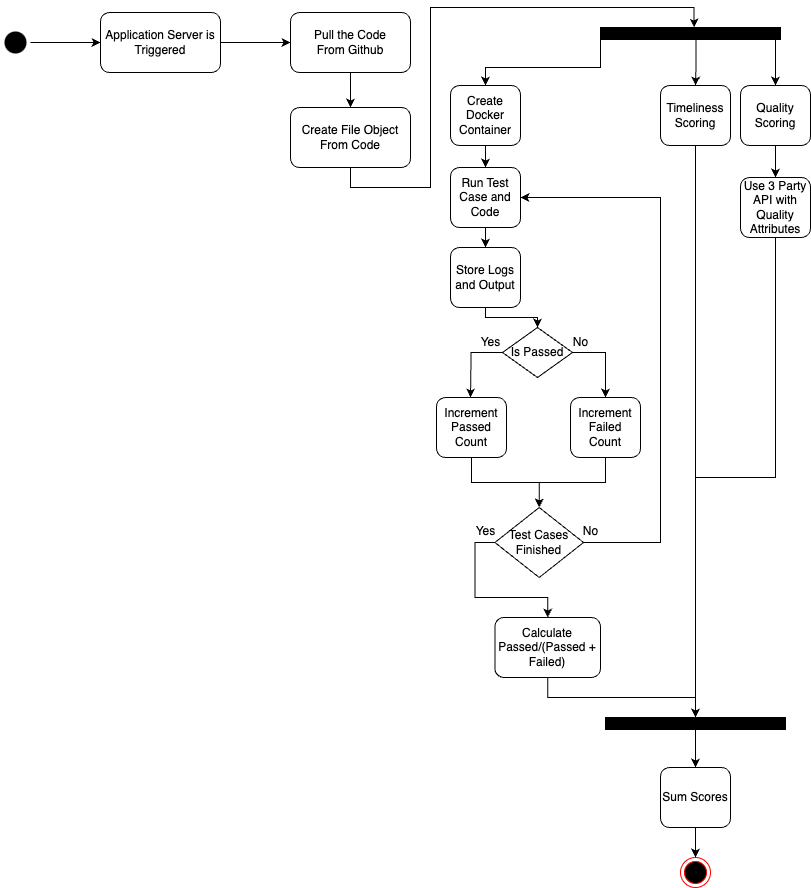
\includegraphics[width=\linewidth]{Images/DD-Sandbox.drawio.png}
    \caption{Submission Scoring}
\end{figure}





%------------------------------------------------------------------------------------------------------------------------------------------------
\clearpage
{\color{Blue}{\section{User Interface Design}}}
\label{sect:ui}
In this section, we present user interfaces for Students and Educators. We created a detailed user interface design to inform the reader from a broader perspective.  It provides a clear understanding of how the end-user will interact with the software. This visual representation can demonstrate the flow and layout of the application, making it easier for stakeholders to grasp the user experience. In the UI design we aim to serve as a common language for all stakeholders, including developers, designers, project managers, and clients. It helps in bridging the gap between non-technical and technical team members with help of graphical demonstration. We tried to create every screen possible in order to inform to developers and stakeholders as much as possible. Developer can simplify and advance this user interface designs if they needed.
\\
Naturally runtime views contain much information however user design shows the application from students and educators. However, every mockup is somehow related to a runtime view. Related runtime views are shown.

\begin{center}
    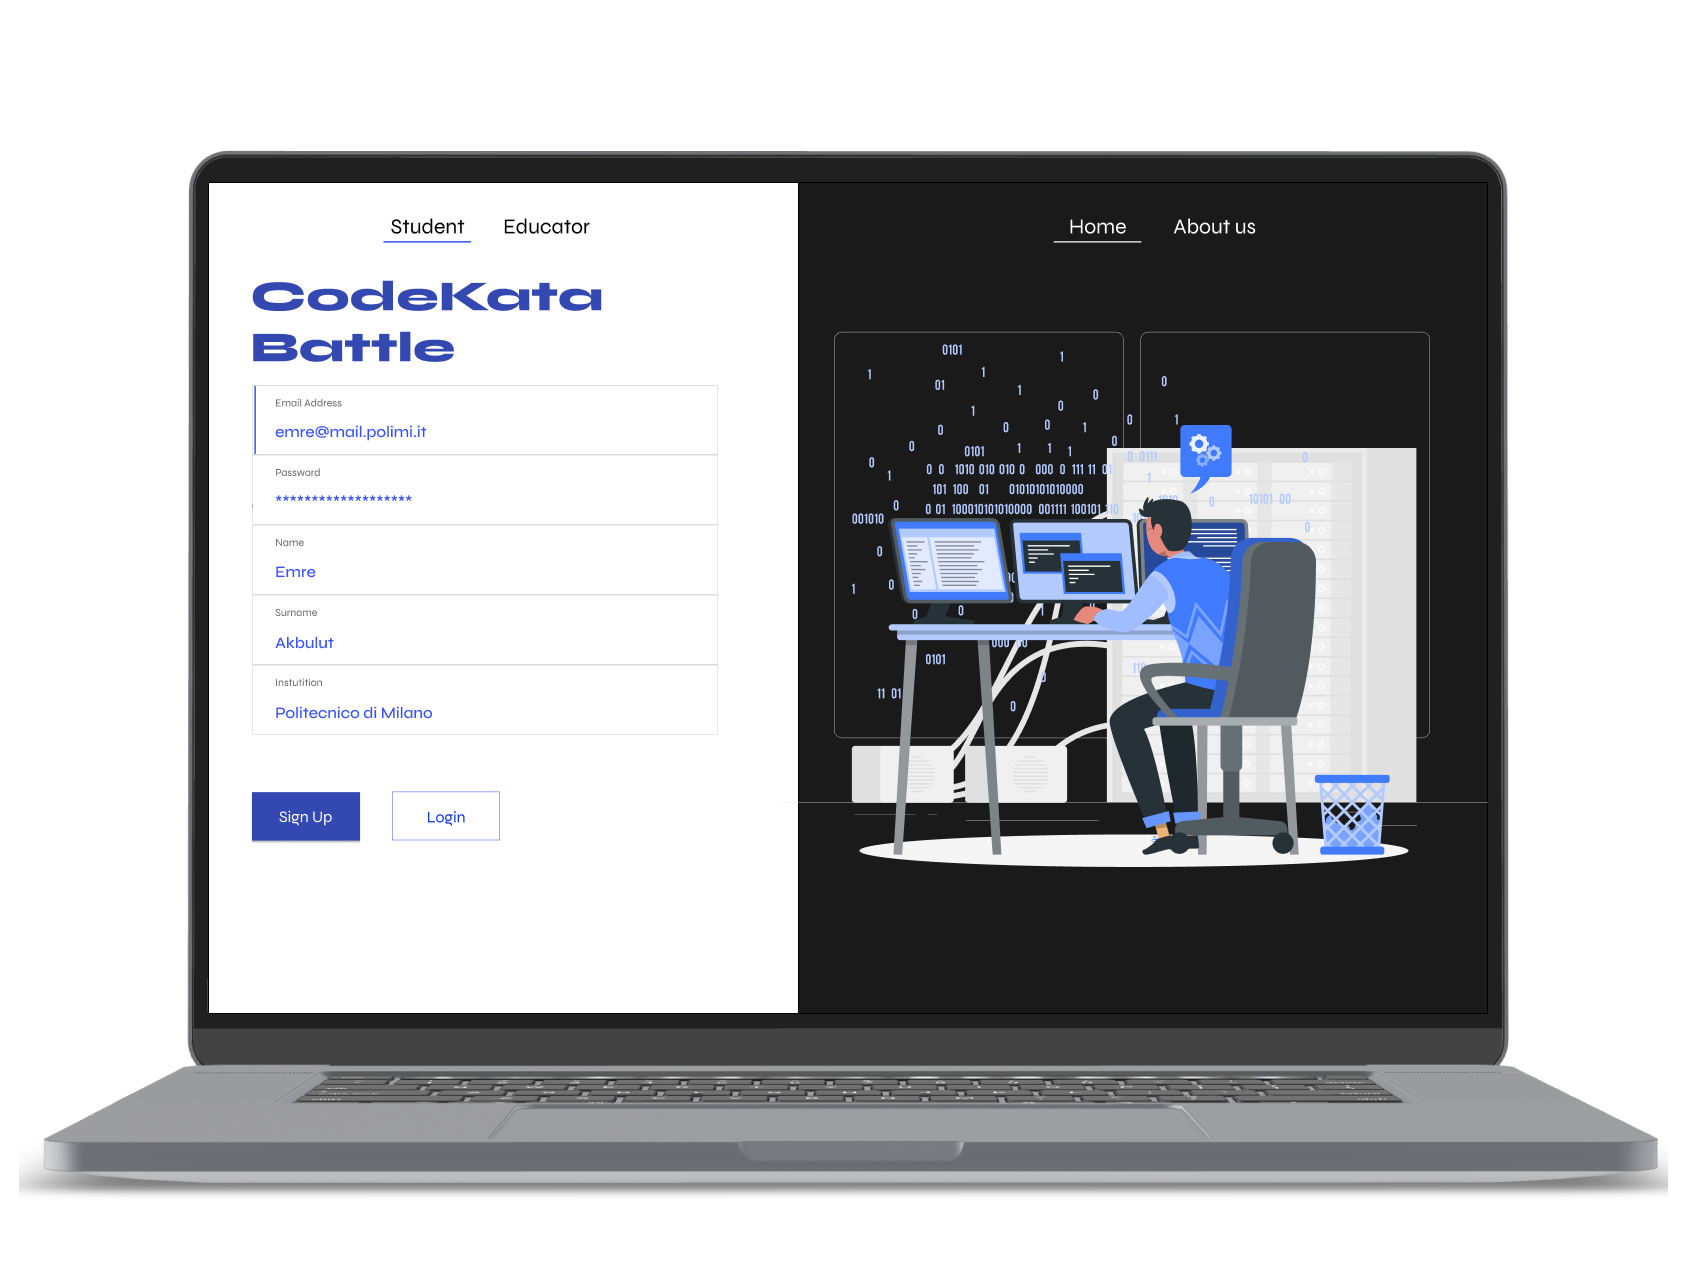
\includegraphics[scale=0.13]{Images/ui-ux/student_signup.png}
    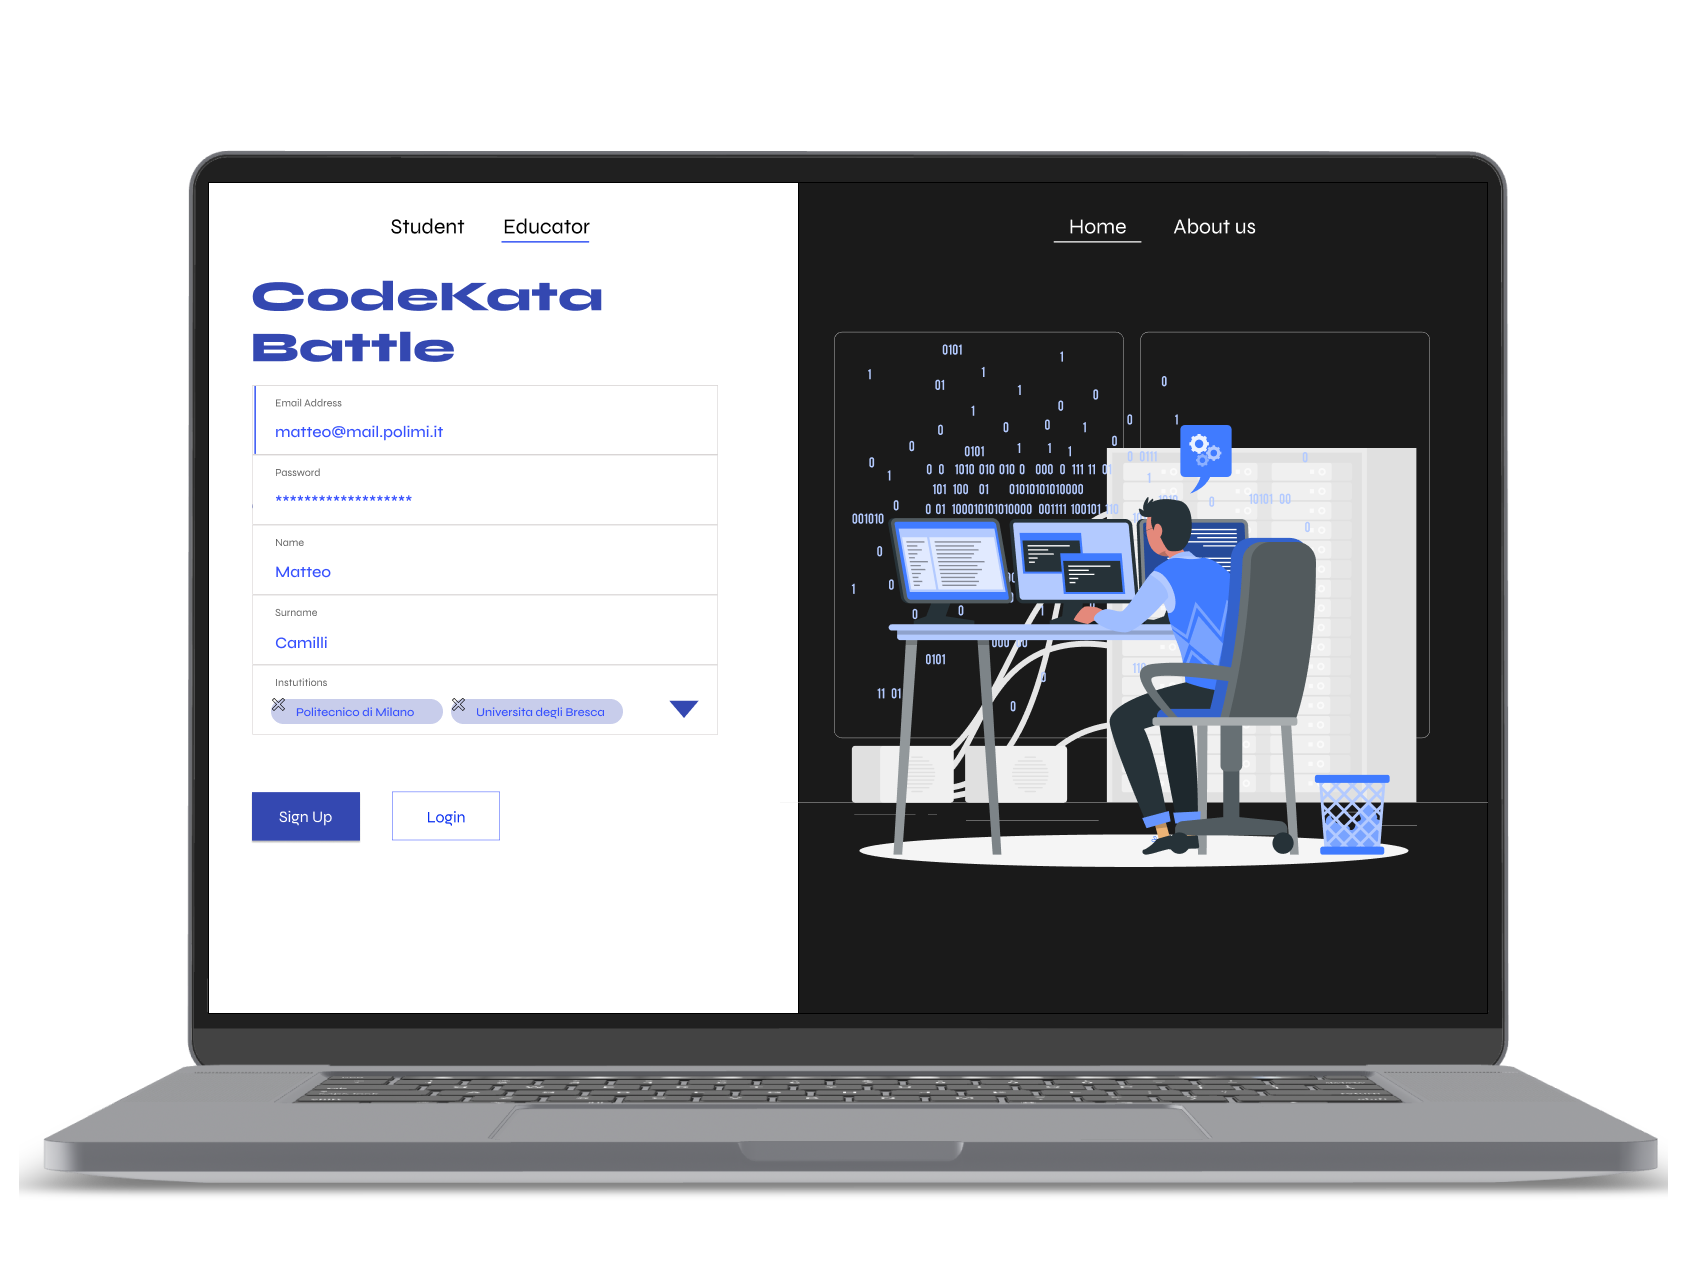
\includegraphics[scale=0.13]{Images/ui-ux/educator_signup.png}
    (a) $UI_{1}$ Sign up Screens 
\end{center}

\begin{center}
    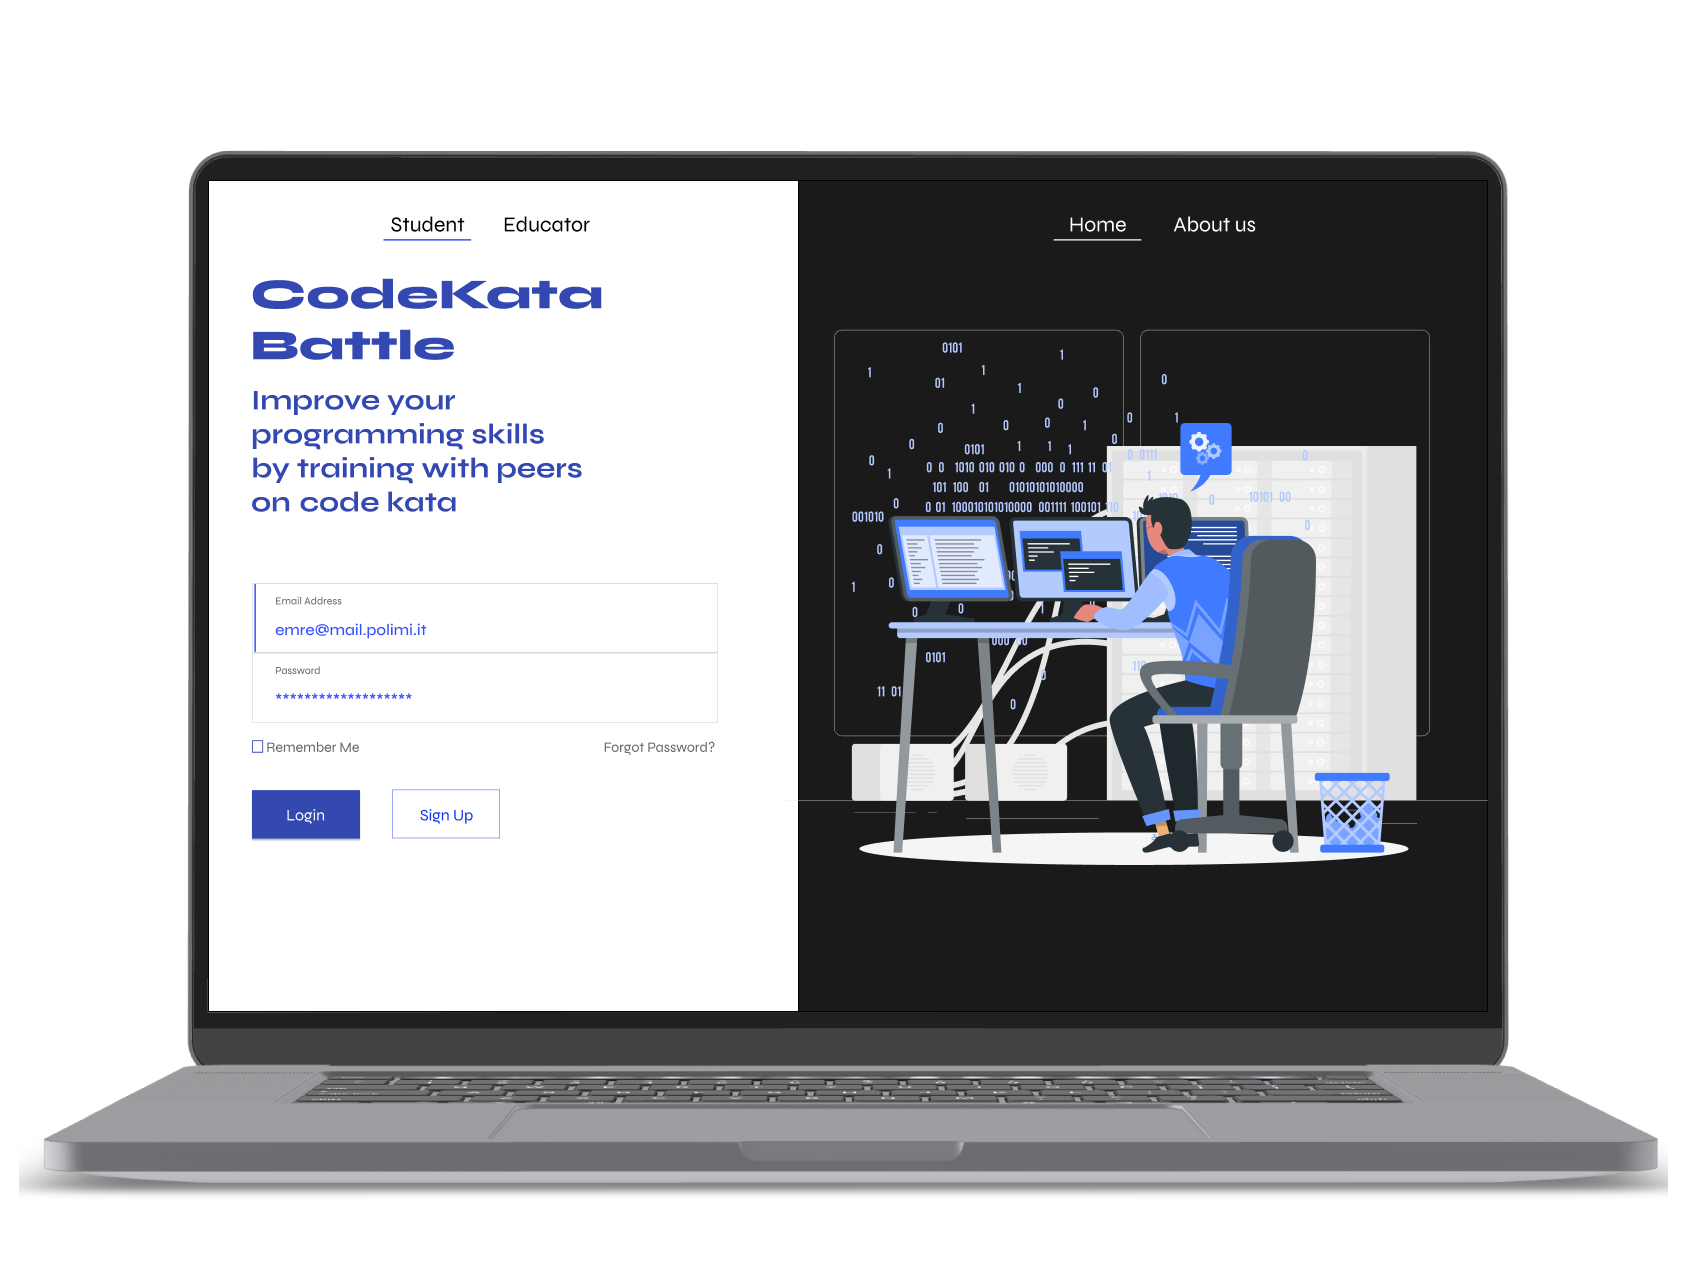
\includegraphics[scale=0.13]{Images/ui-ux/student_login.png}
    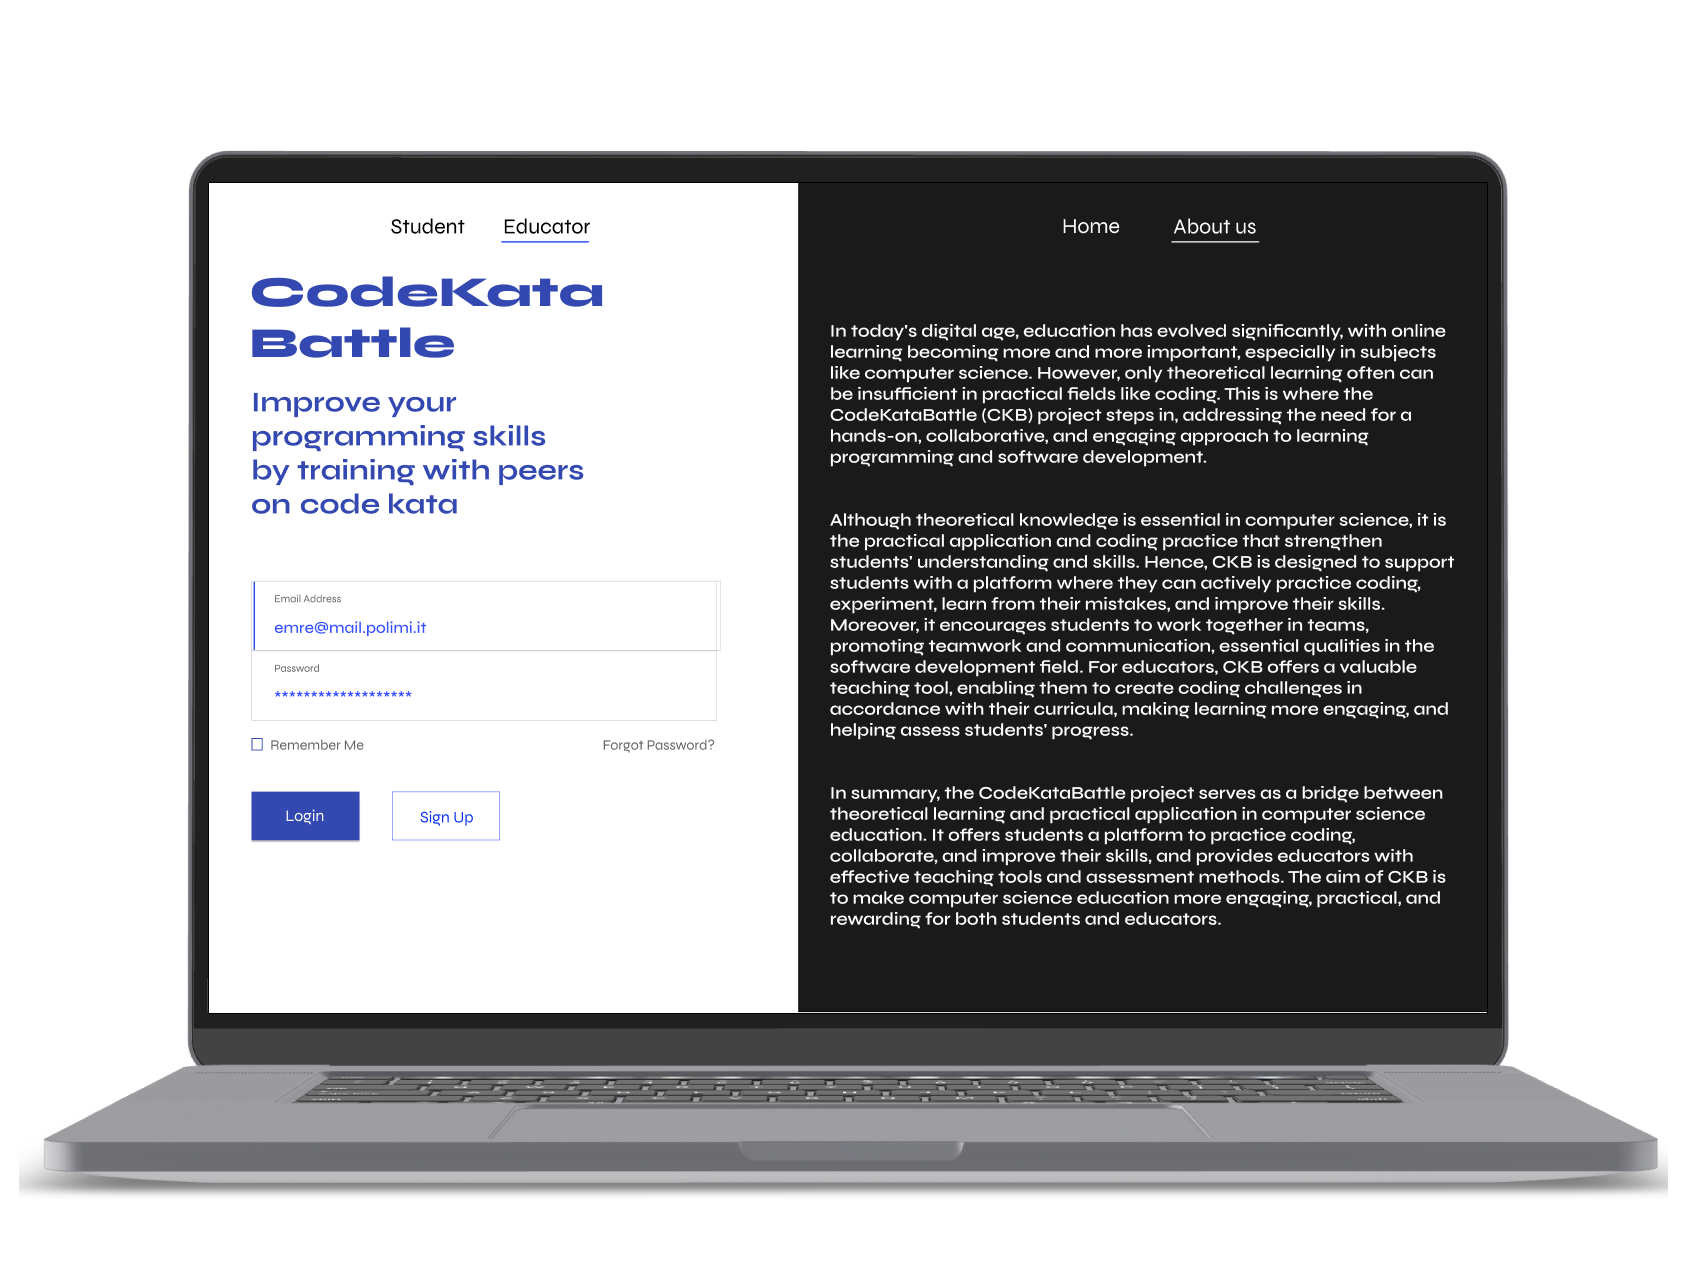
\includegraphics[scale=0.13]{Images/ui-ux/educator_login.png}
\end{center}
    \begin{center}
        (b) $UI_{2}$ Login Screens
    \end{center}

\newpage
\begin{center}
    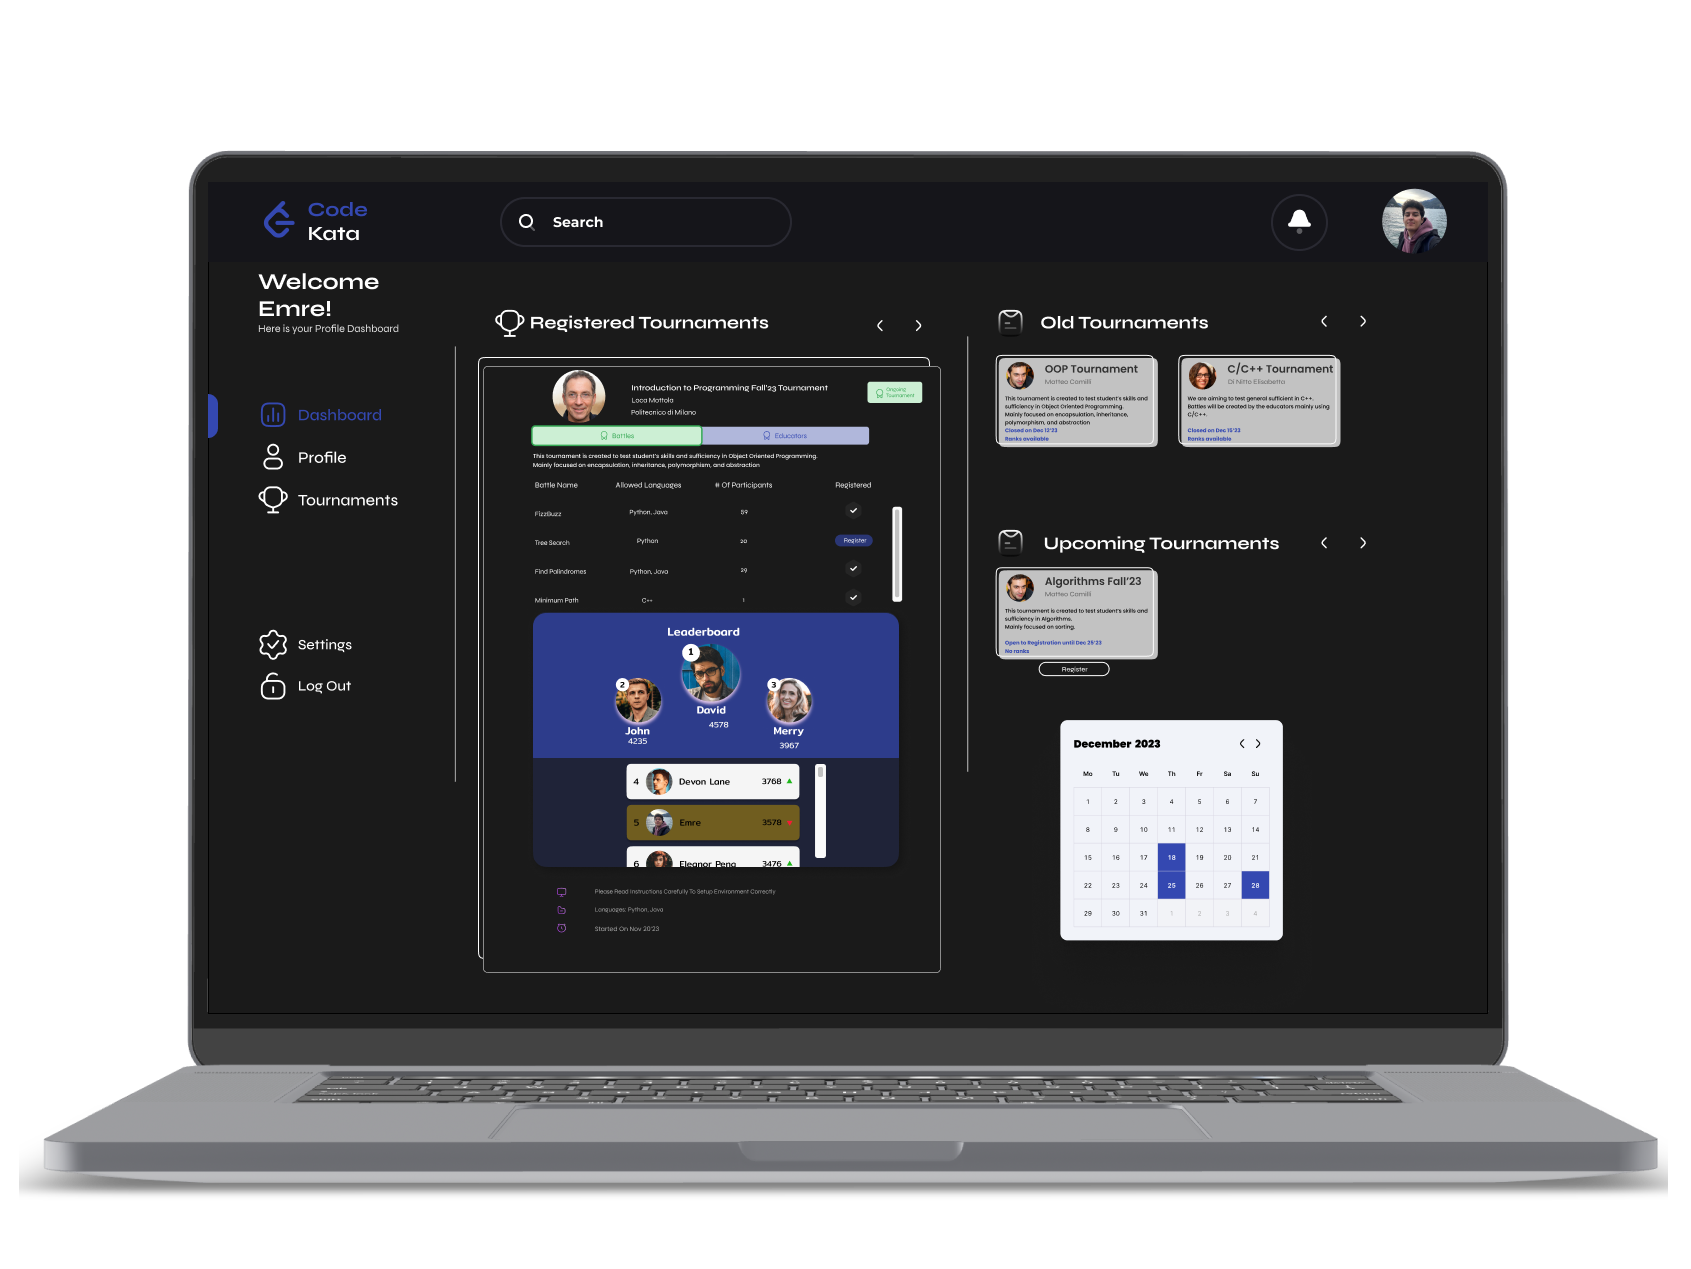
\includegraphics[scale=0.13]{Images/ui-ux/student_dashboard_1.png}
    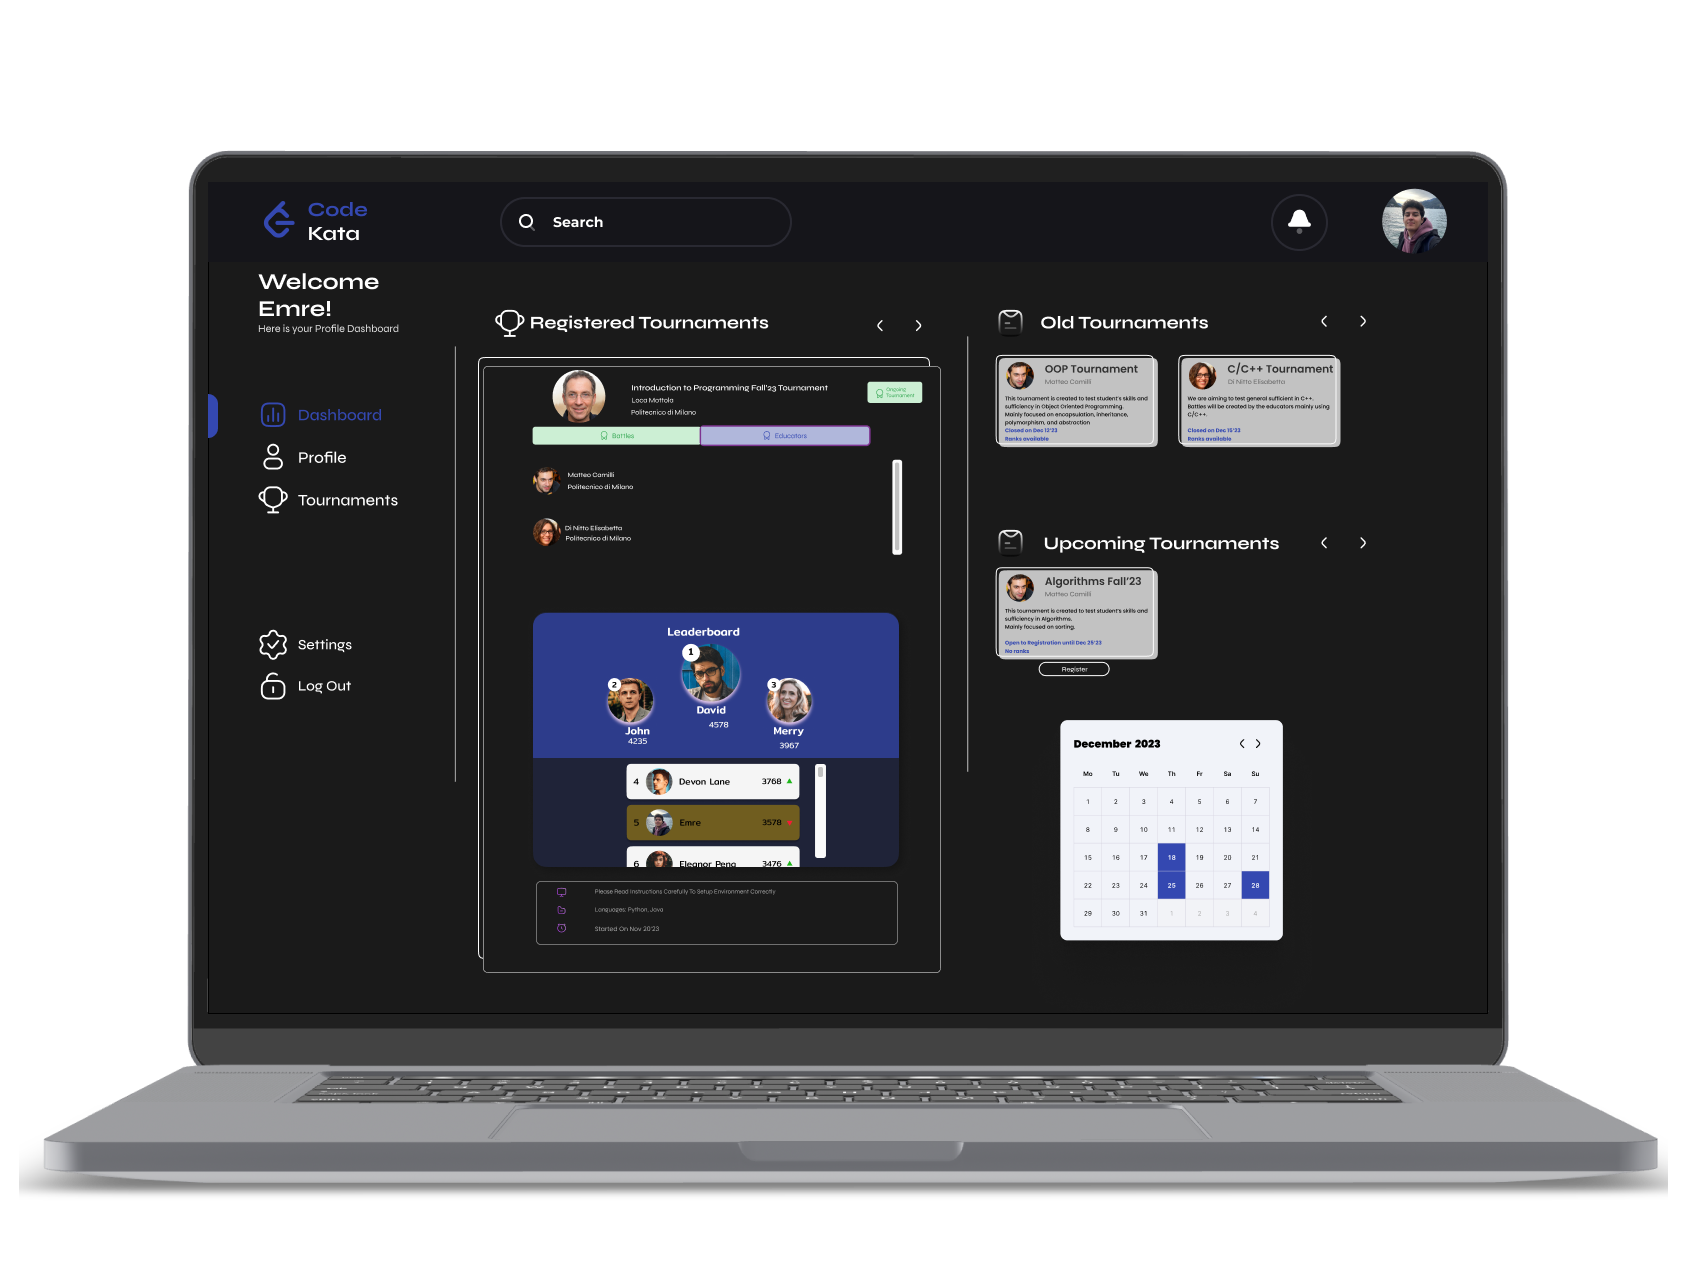
\includegraphics[scale=0.13]{Images/ui-ux/student_dashboard_2.png}
        (c) $UI_{3}$ Student Dashboard
\end{center}
\begin{center}
    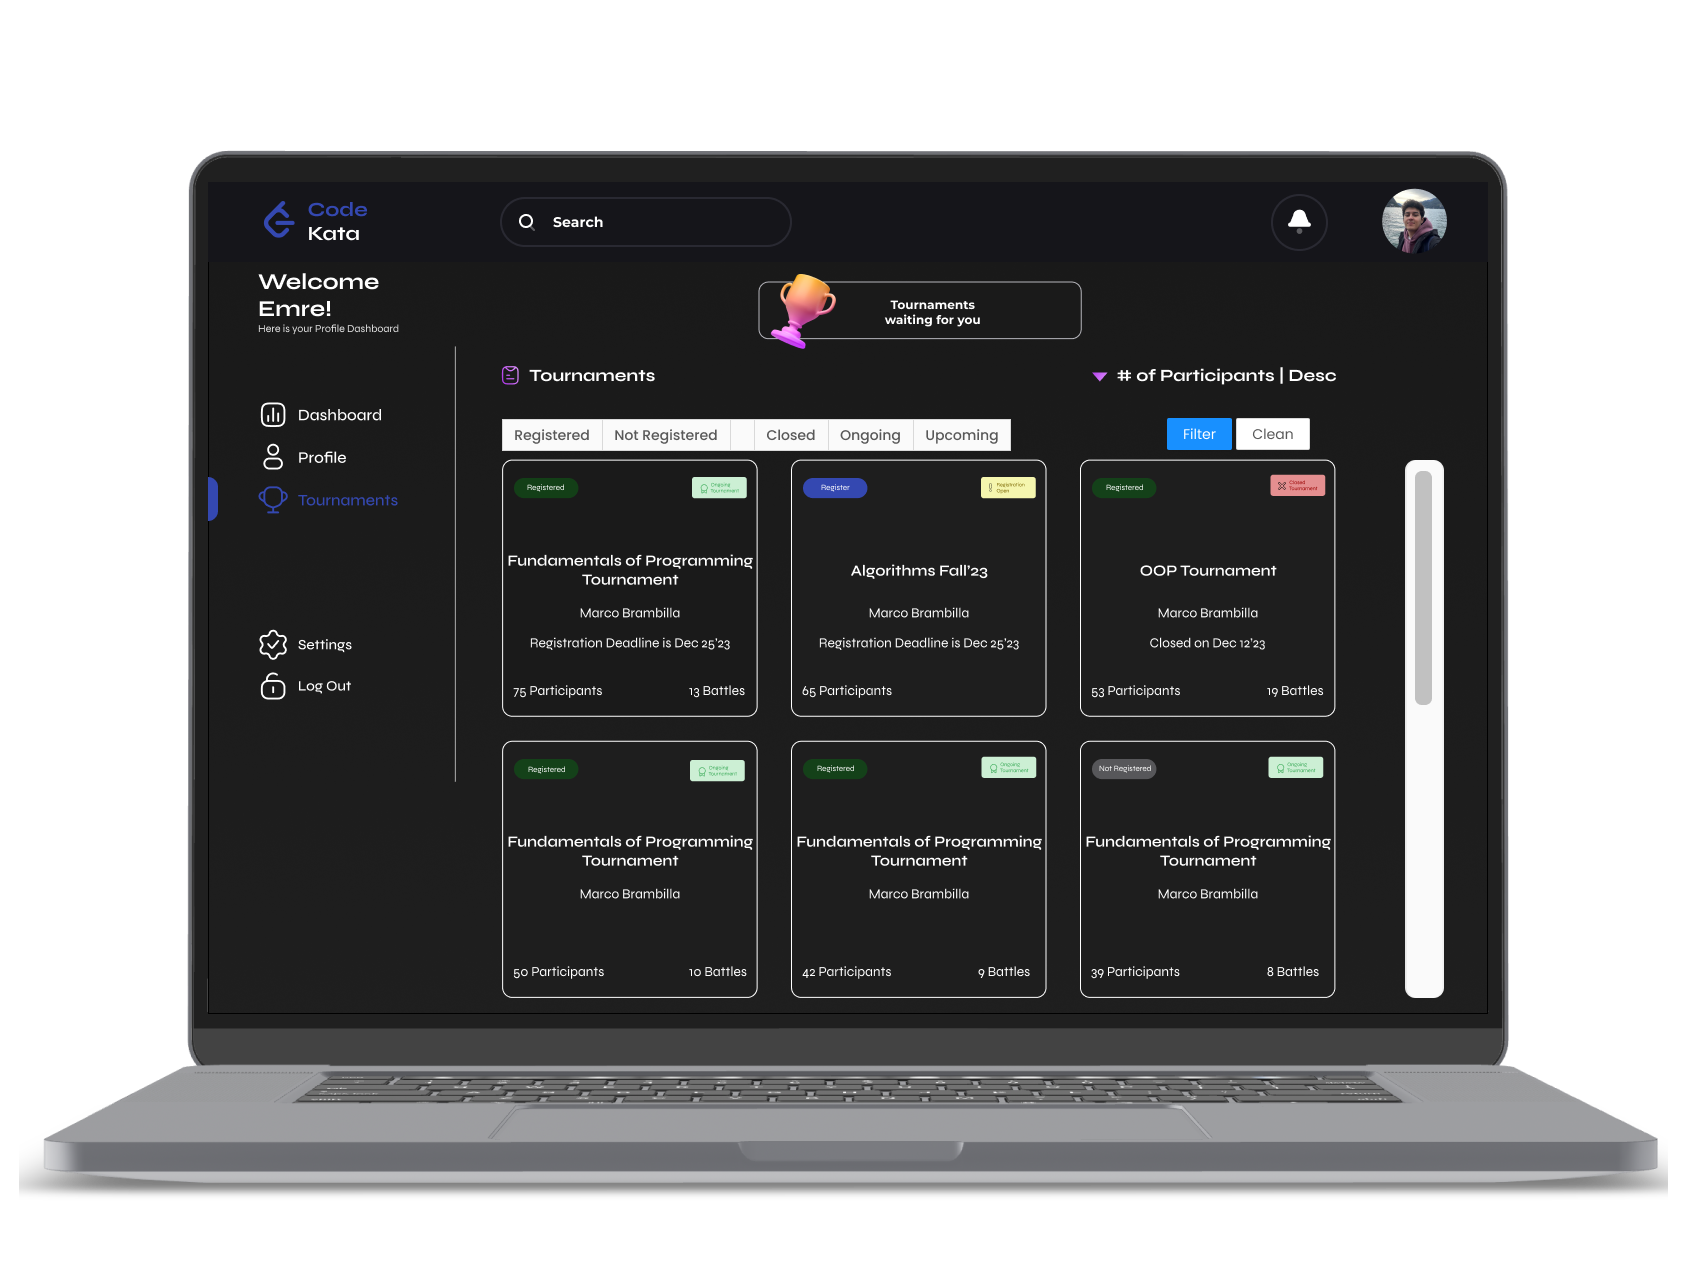
\includegraphics[scale=0.13]{Images/ui-ux/student_tournaments_1.png}
    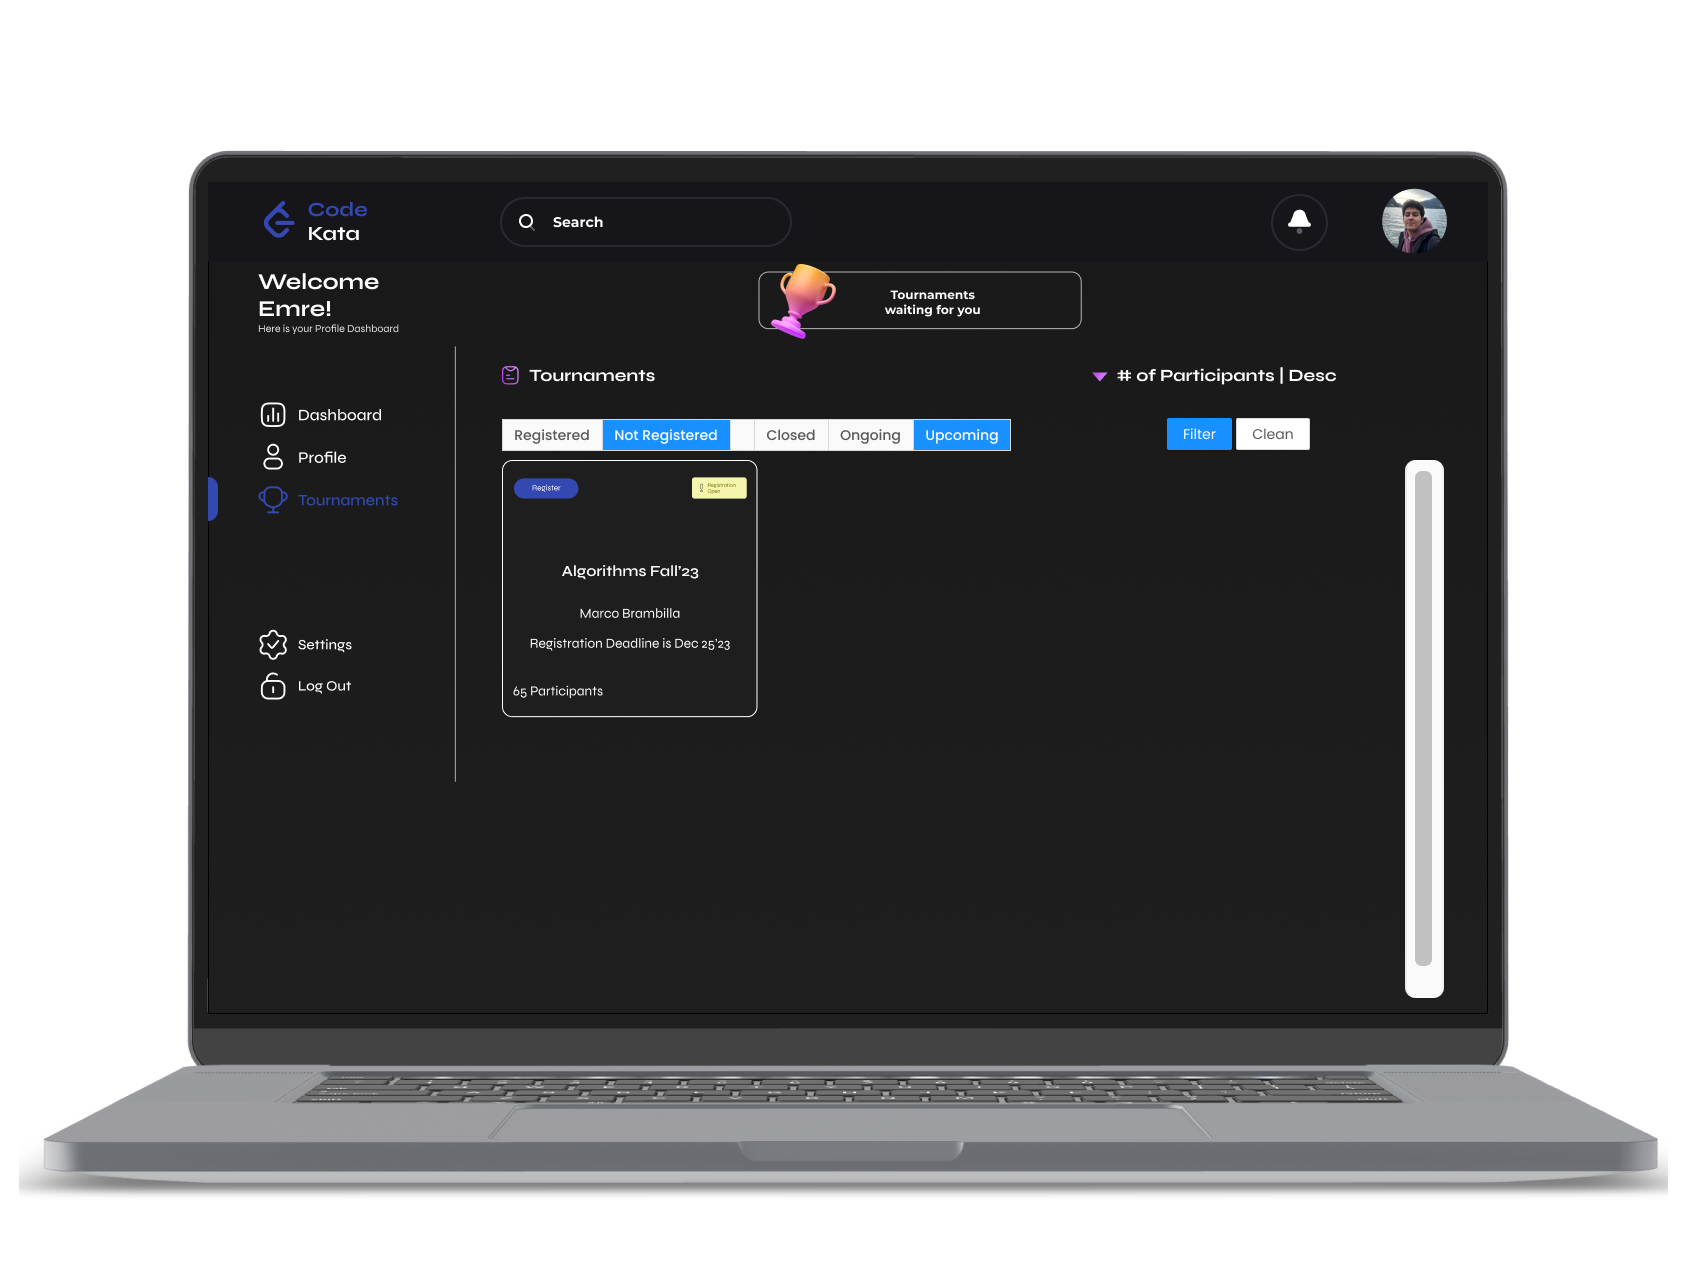
\includegraphics[scale=0.13]{Images/ui-ux/student_tournaments_2.png}    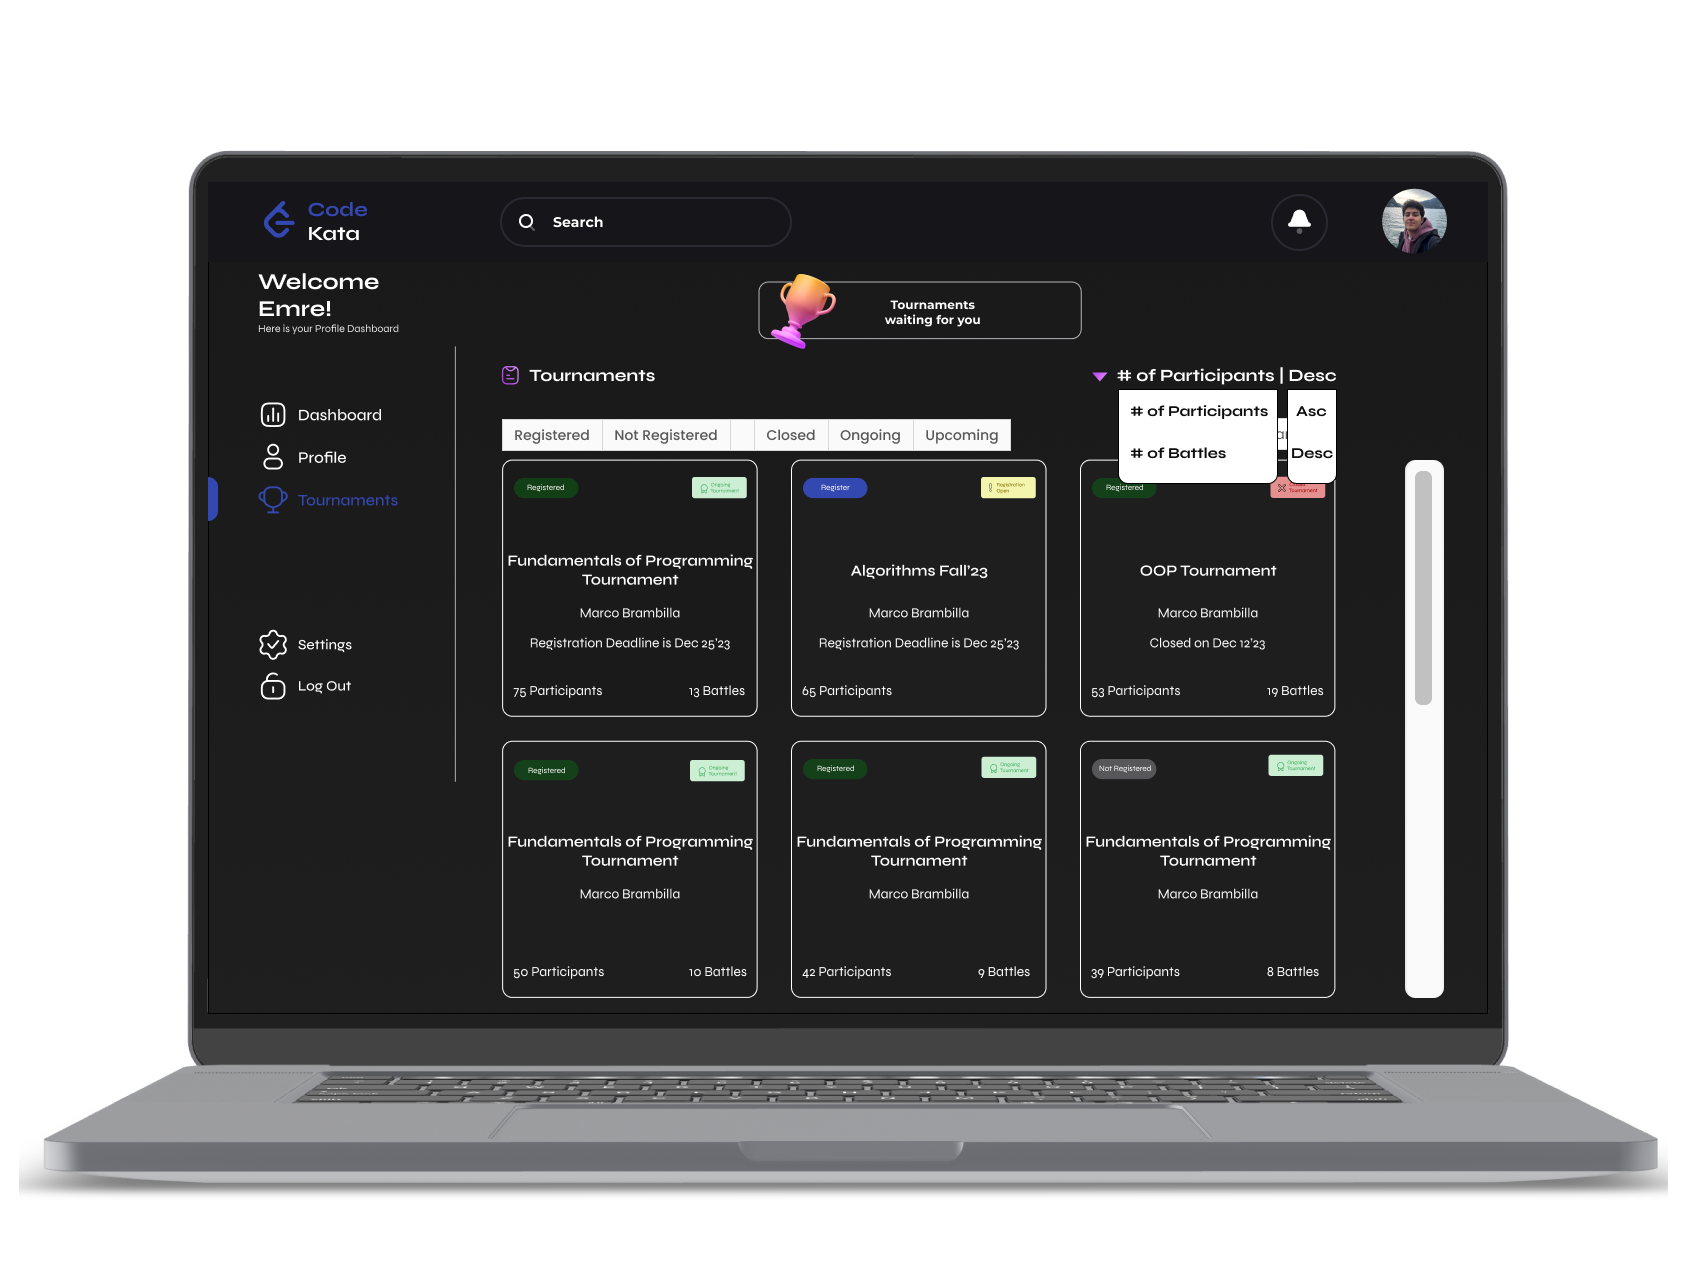
\includegraphics[scale=0.13]{Images/ui-ux/student_tournaments_3.png}    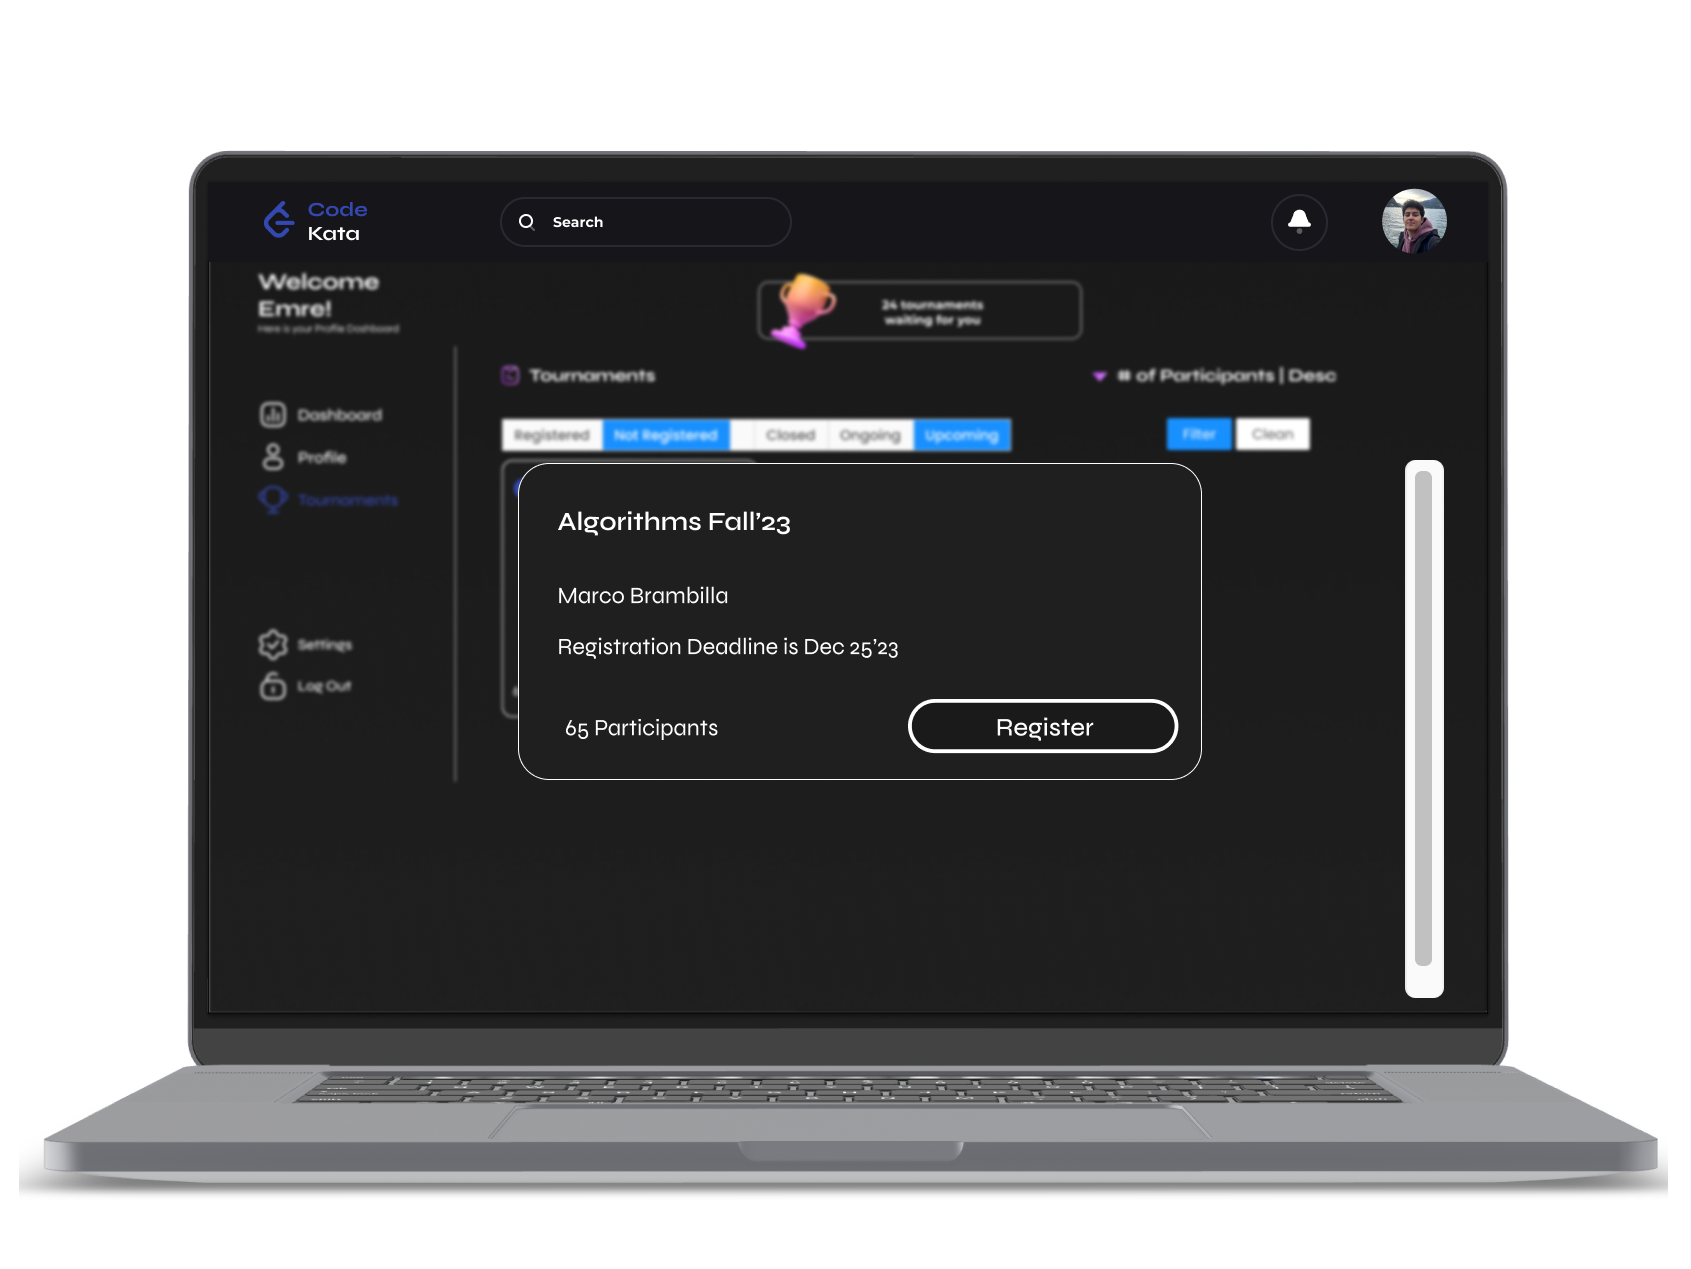
\includegraphics[scale=0.13]{Images/ui-ux/student_tournaments_4.png}
        (d) $UI_{4}$ Student Tournaments Page
\end{center}

\begin{center}
    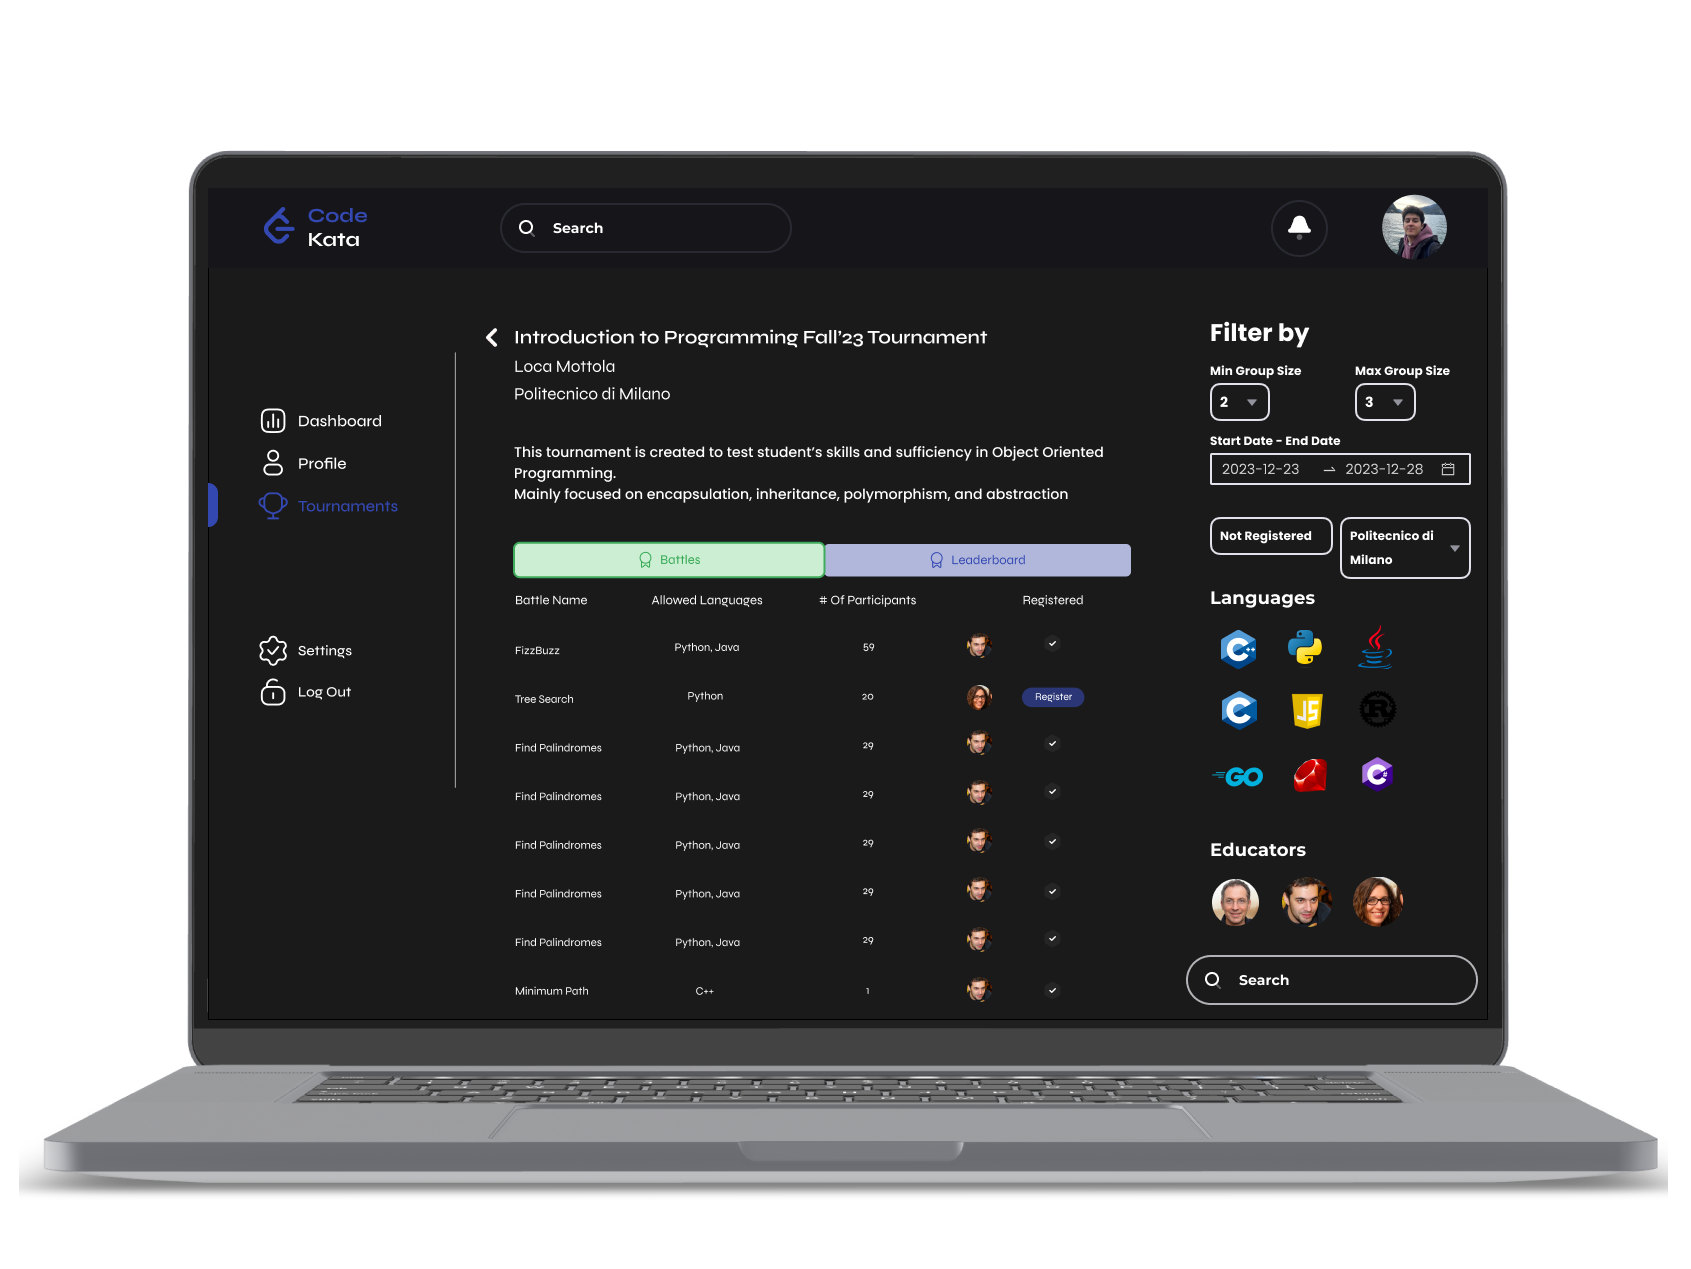
\includegraphics[scale=0.13]{Images/ui-ux/student_tournament_1.png}
    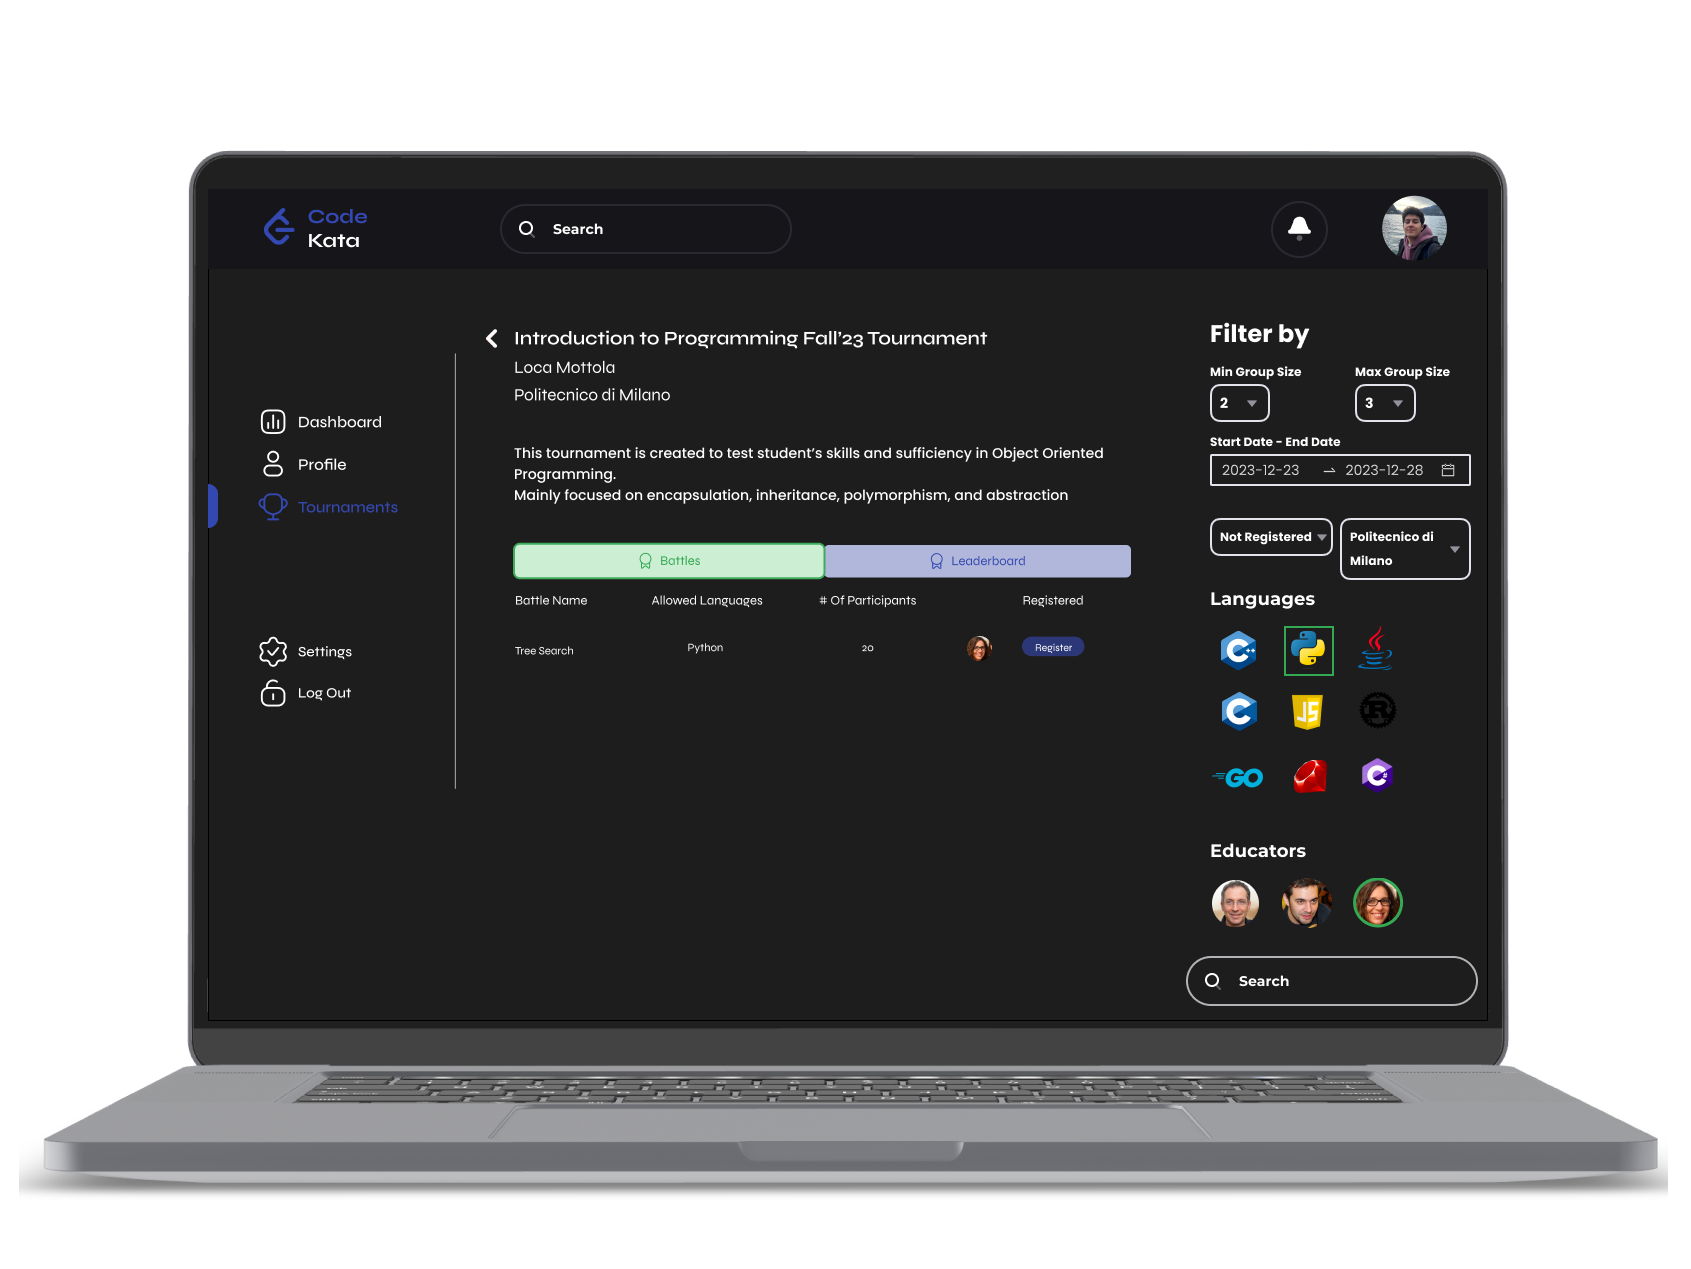
\includegraphics[scale=0.13]{Images/ui-ux/student_tournament_2.png}    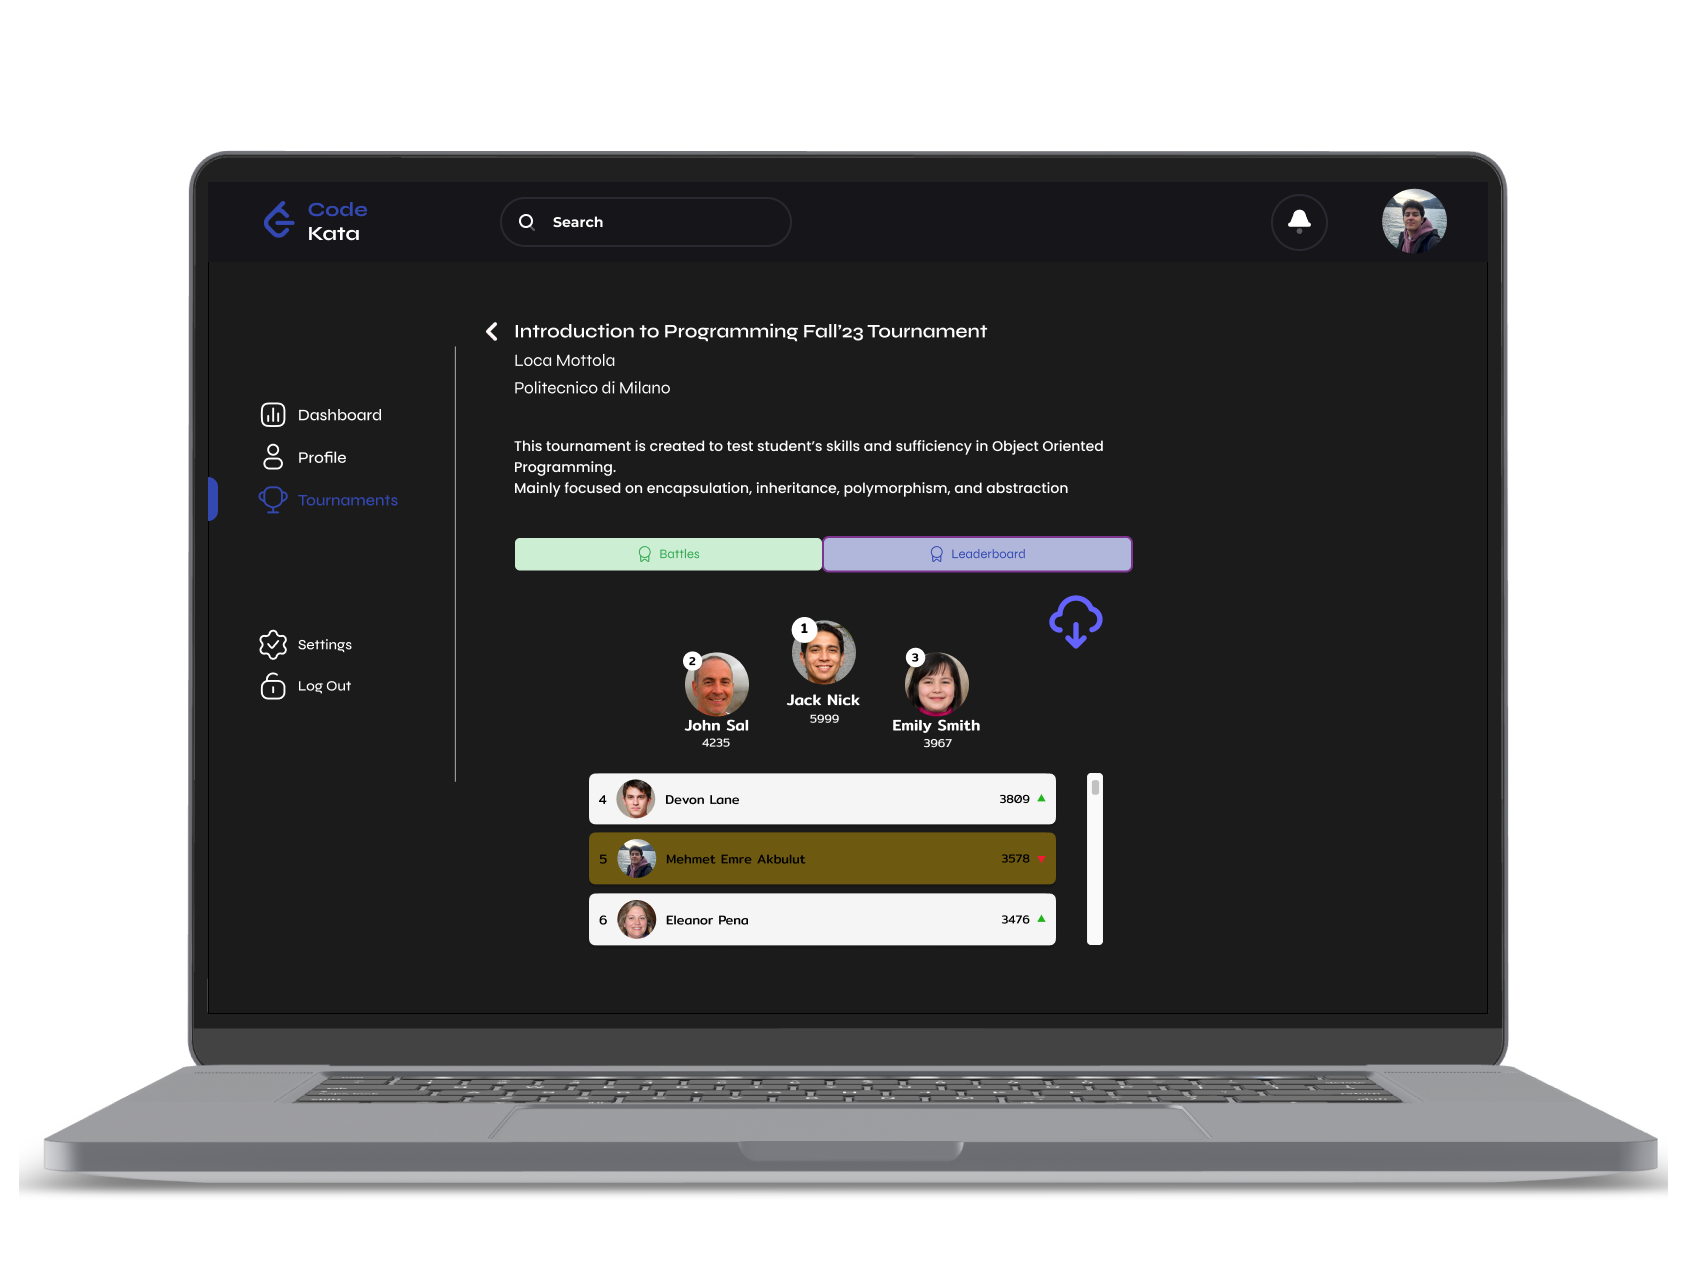
\includegraphics[scale=0.13]{Images/ui-ux/student_tournament_3.png} 
    \\ (e) $UI_{5}$ Student visits a Tournament 
\end{center}
\newpage
\begin{center}
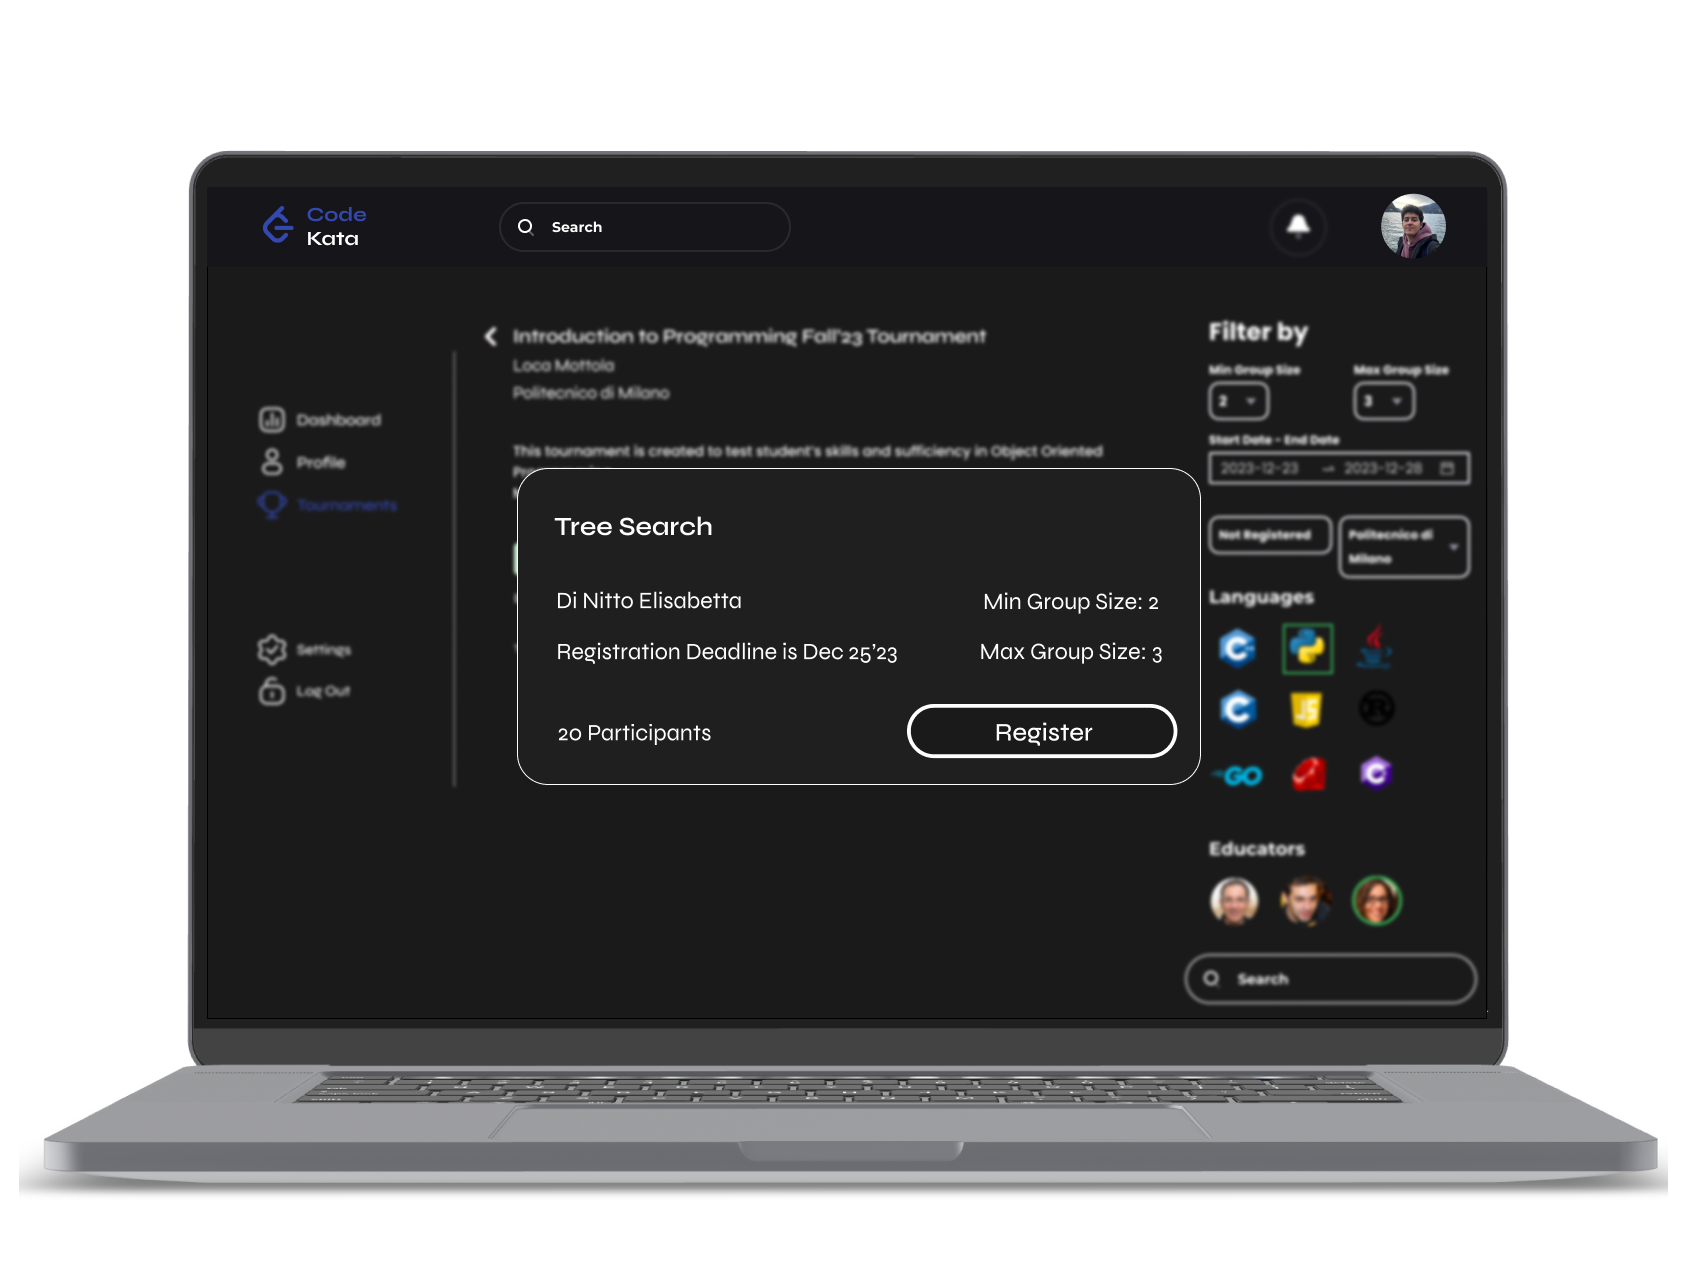
\includegraphics[scale=0.13]{Images/ui-ux/student_battle_register_1.png}
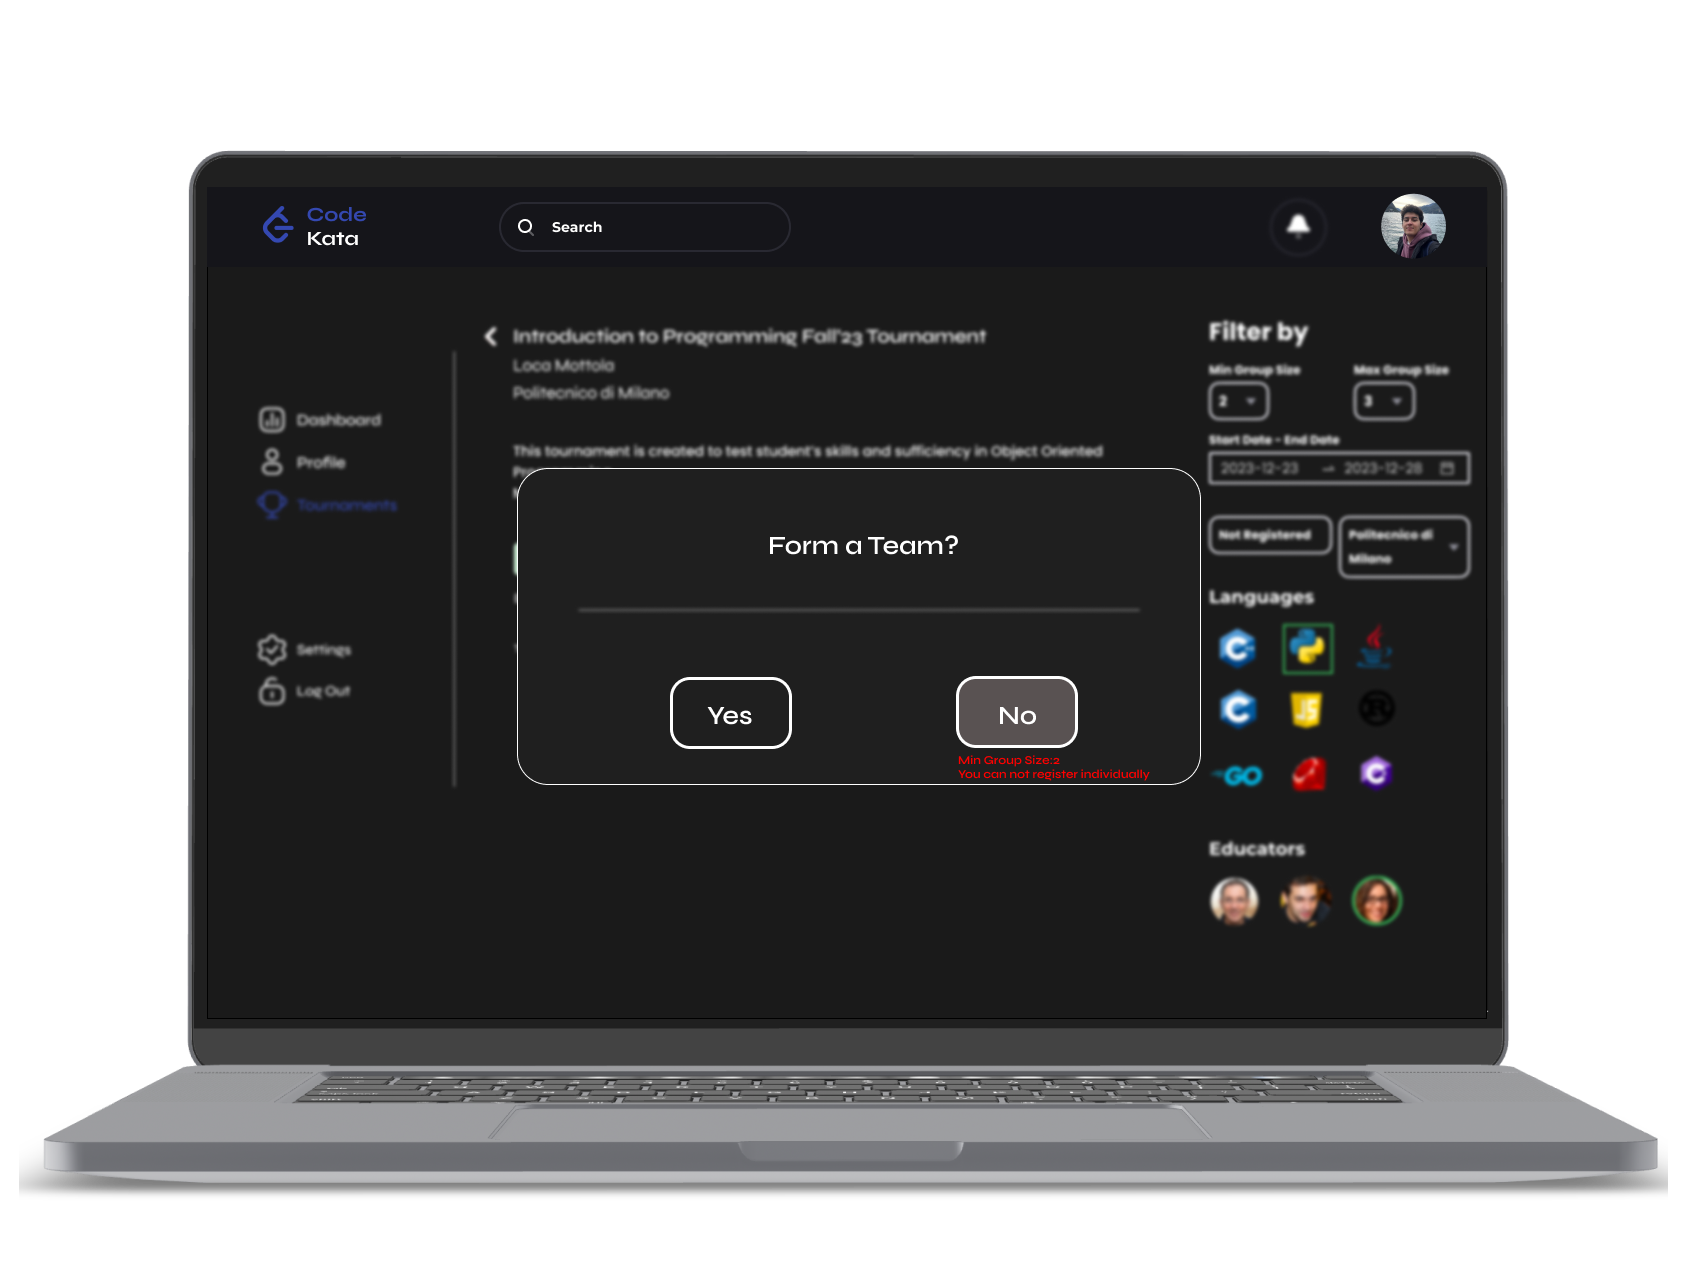
\includegraphics[scale=0.13]{Images/ui-ux/student_battle_register_2.png}
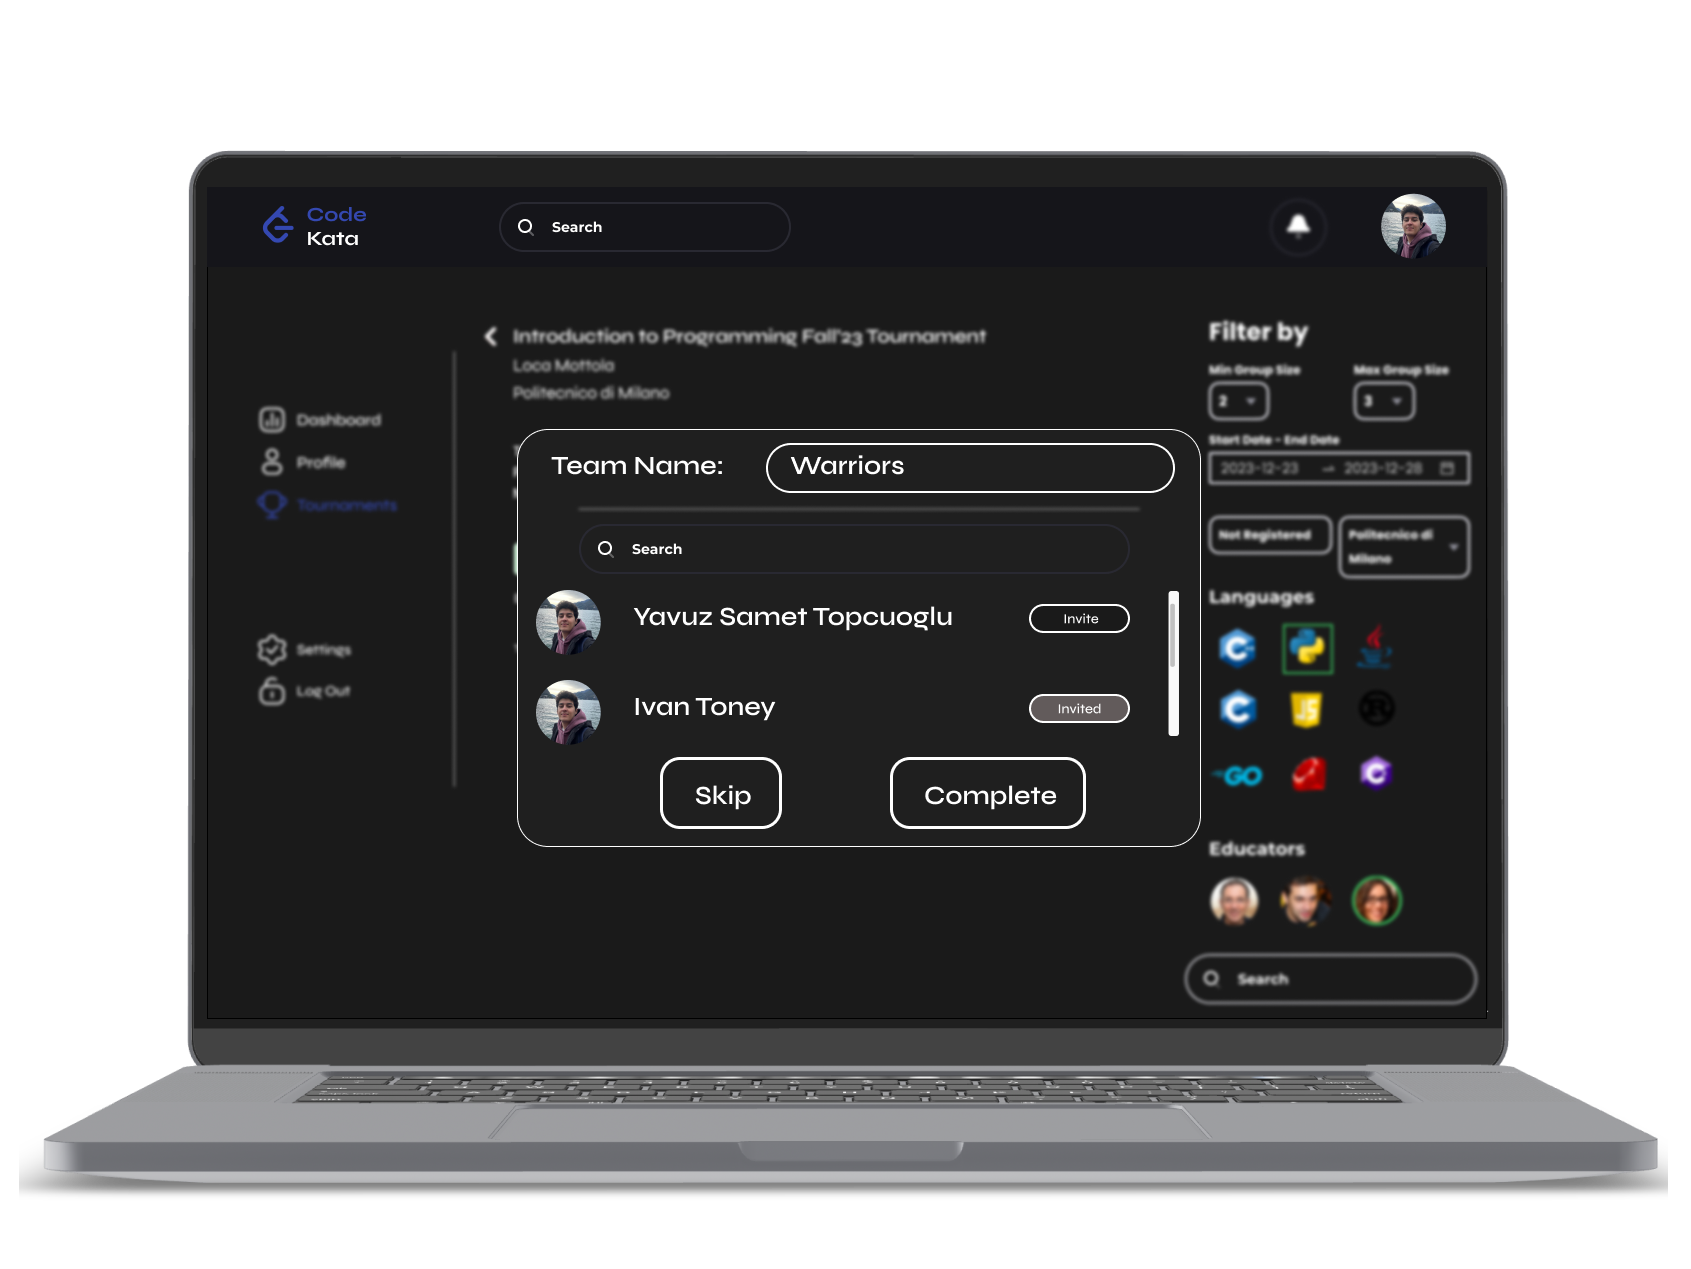
\includegraphics[scale=0.13]{Images/ui-ux/student_battle_register_3.png}
\\ (f) $UI_{6}$  Student Registers Battle 
\end{center}
\newpage
\begin{center}
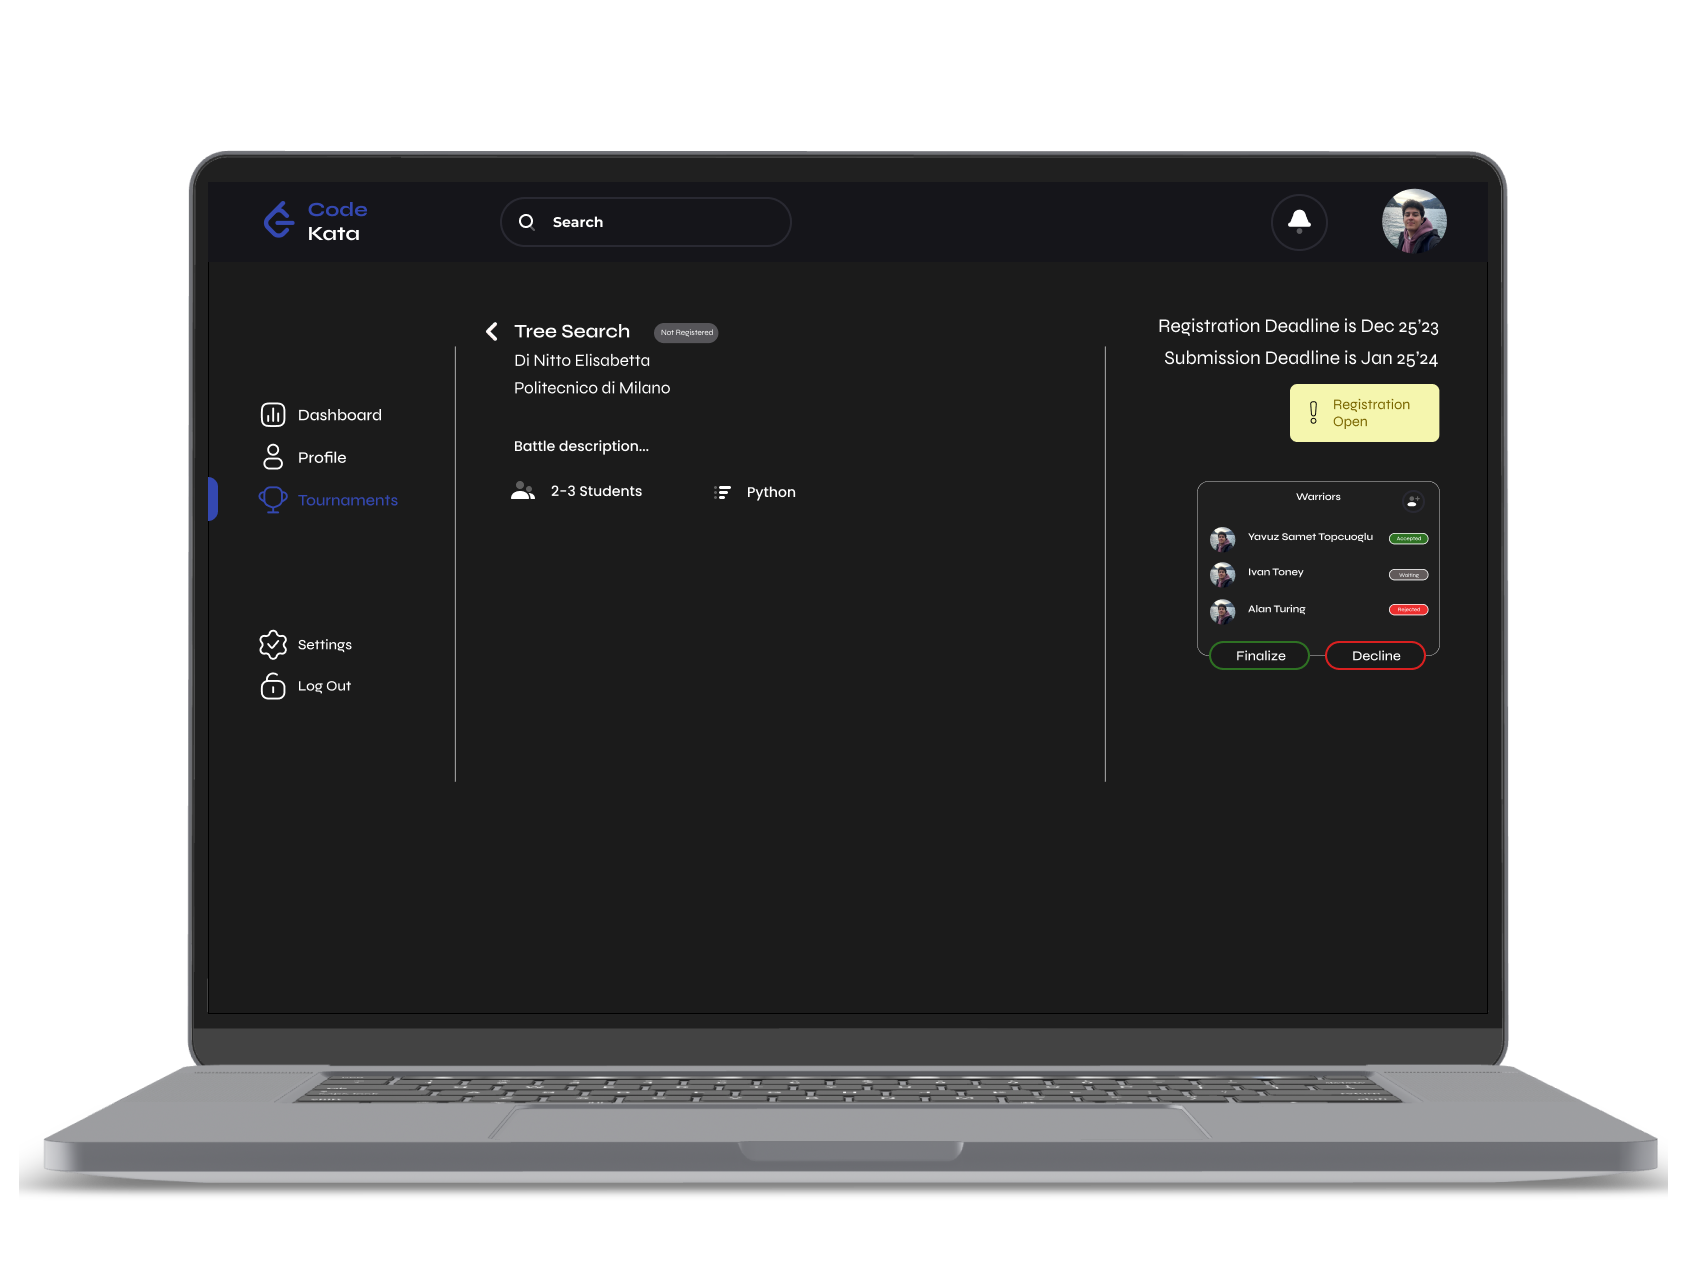
\includegraphics[scale=0.13]{Images/ui-ux/student_battle_1.png}
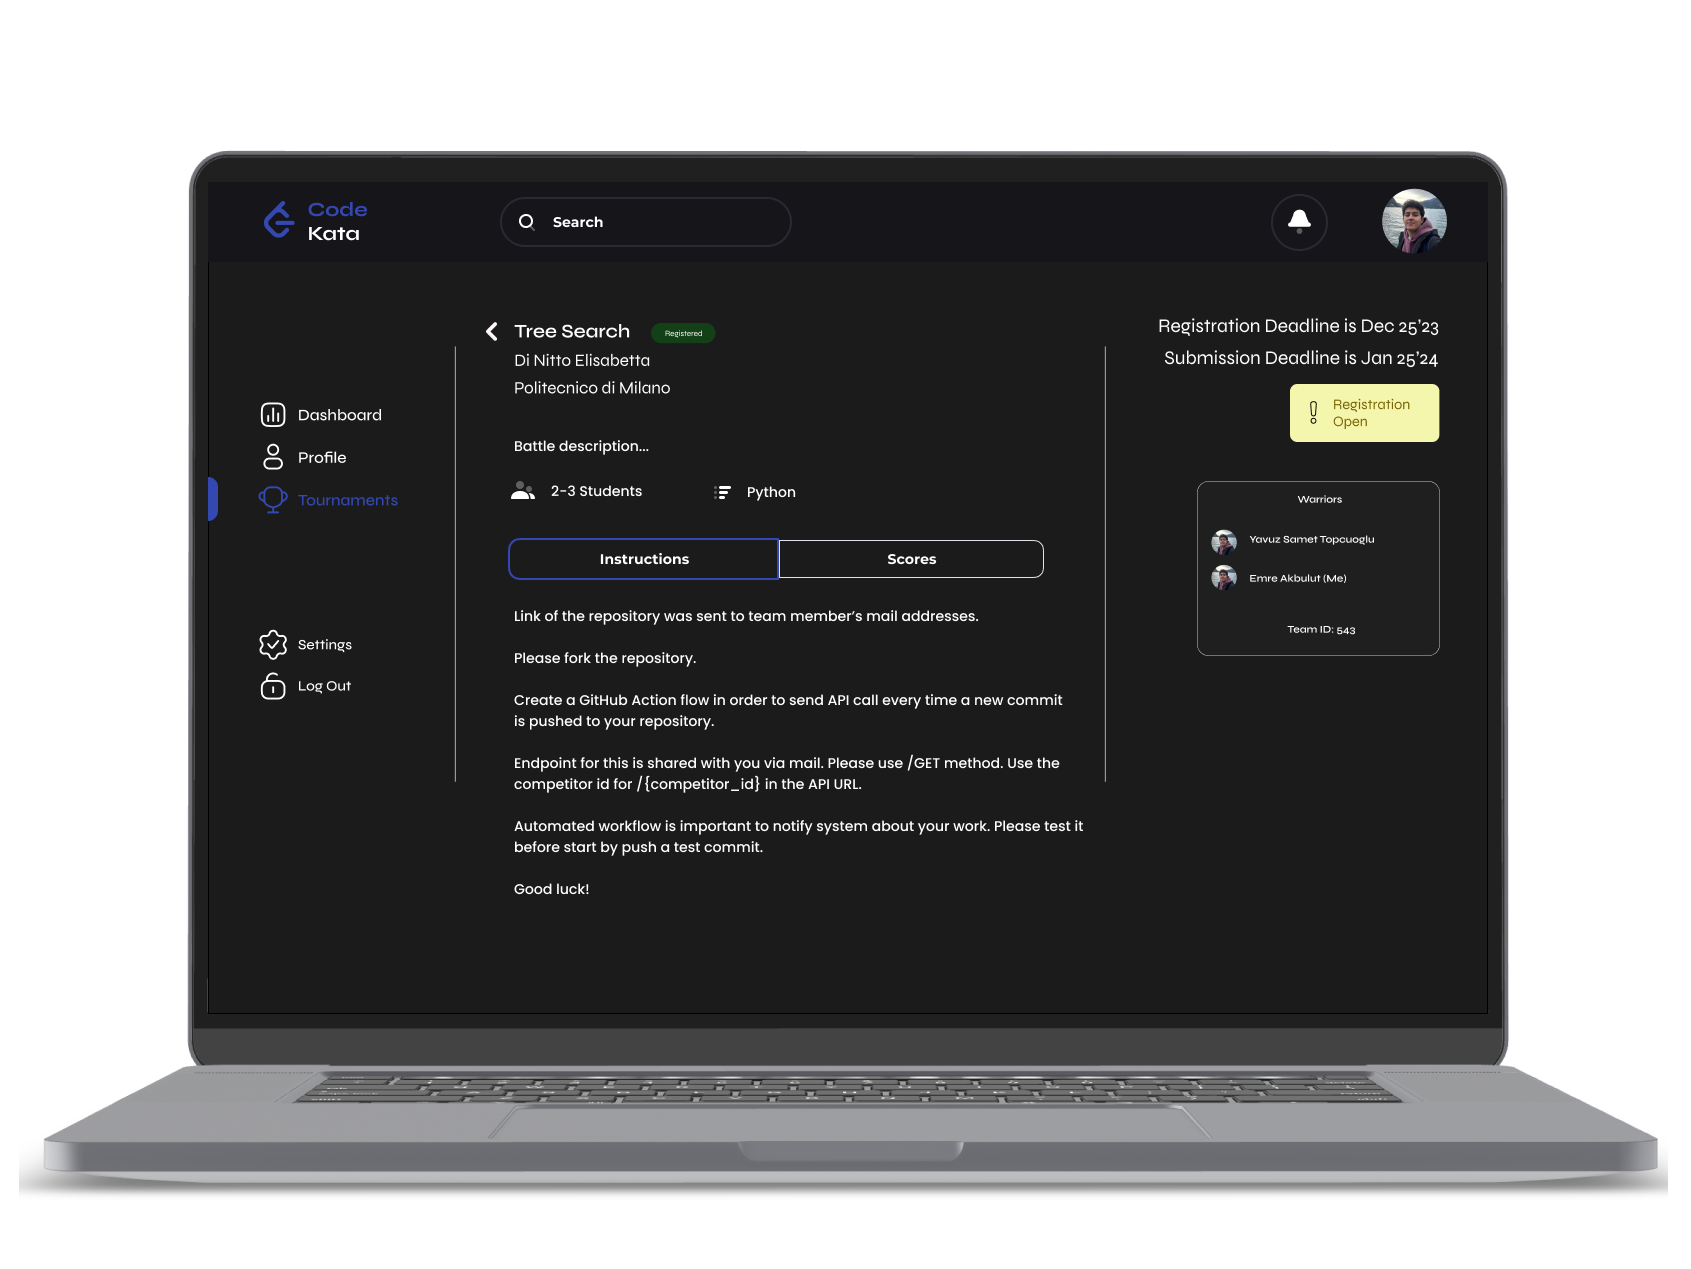
\includegraphics[scale=0.13]{Images/ui-ux/student_battle_2.png}
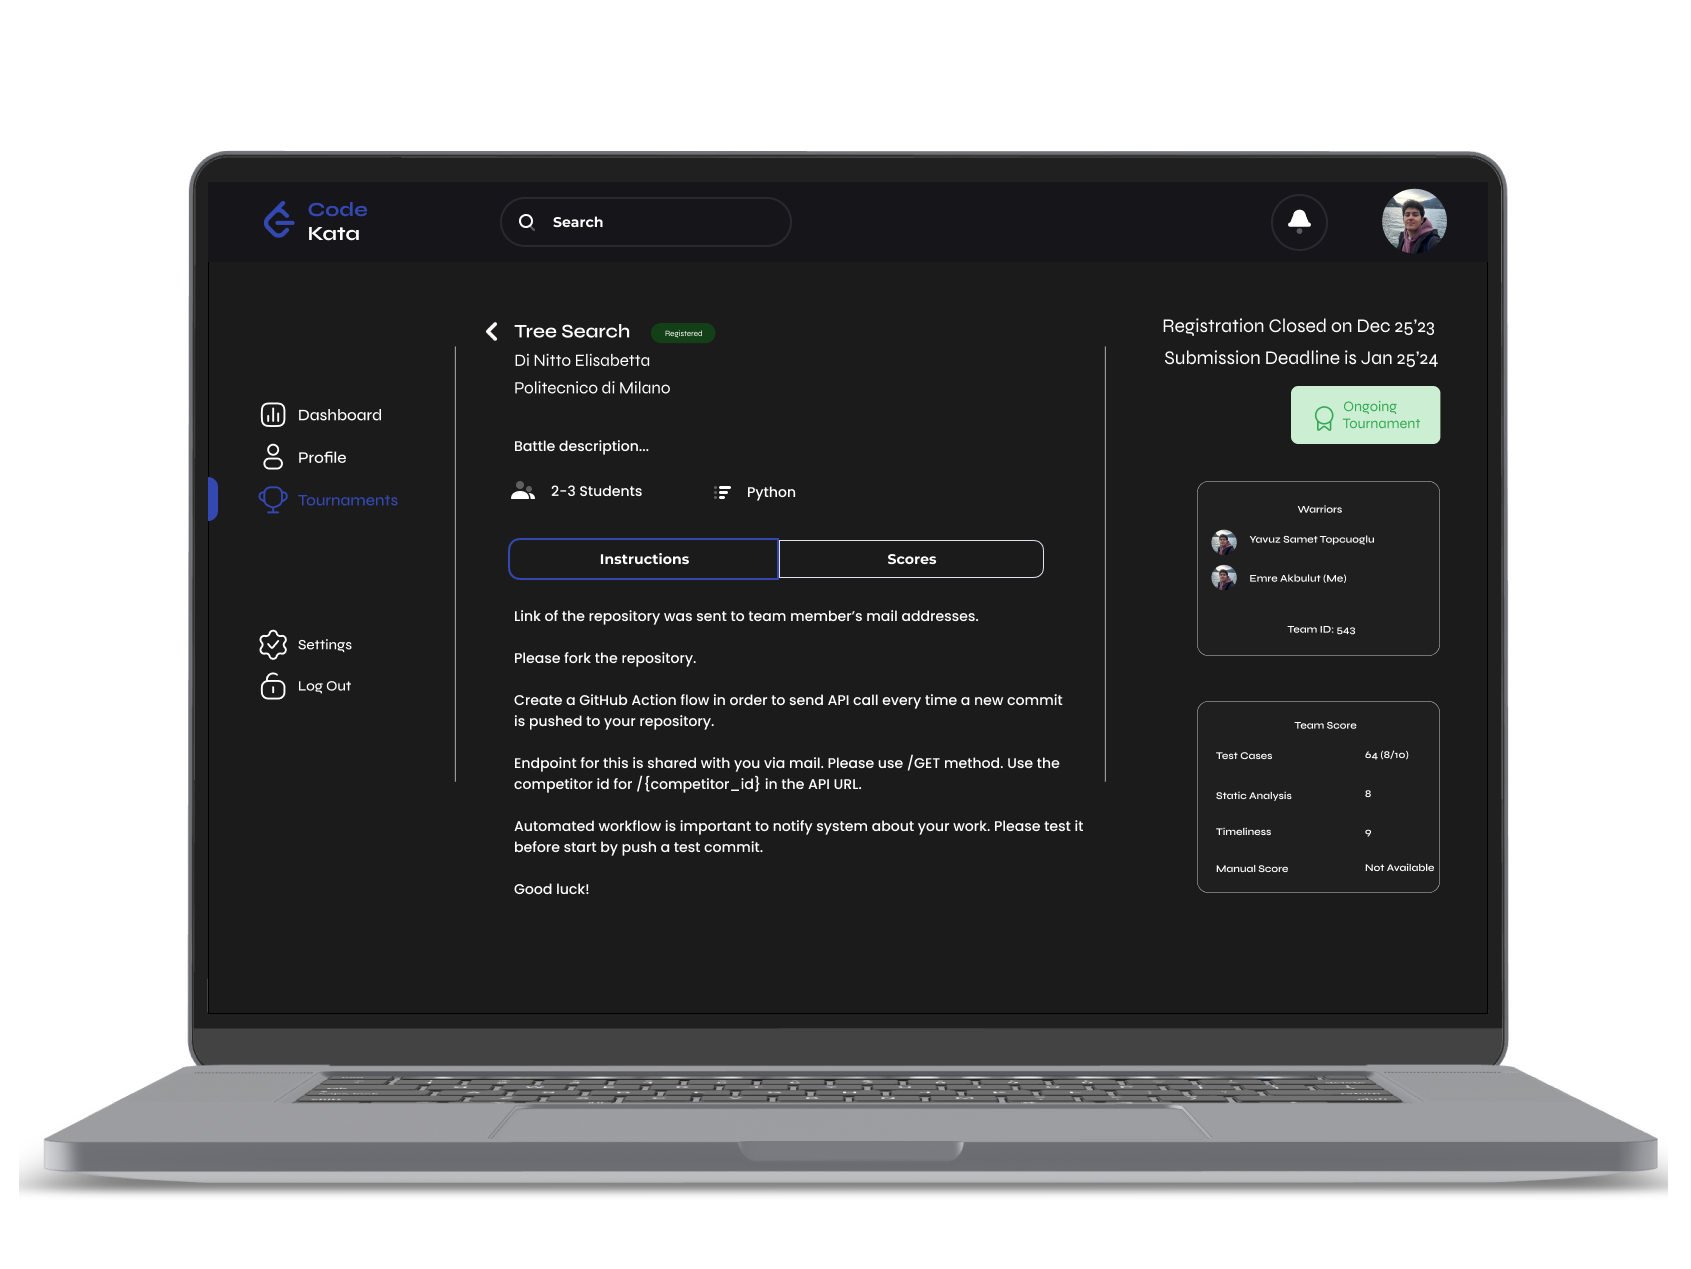
\includegraphics[scale=0.13]{Images/ui-ux/student_battle_3.png}
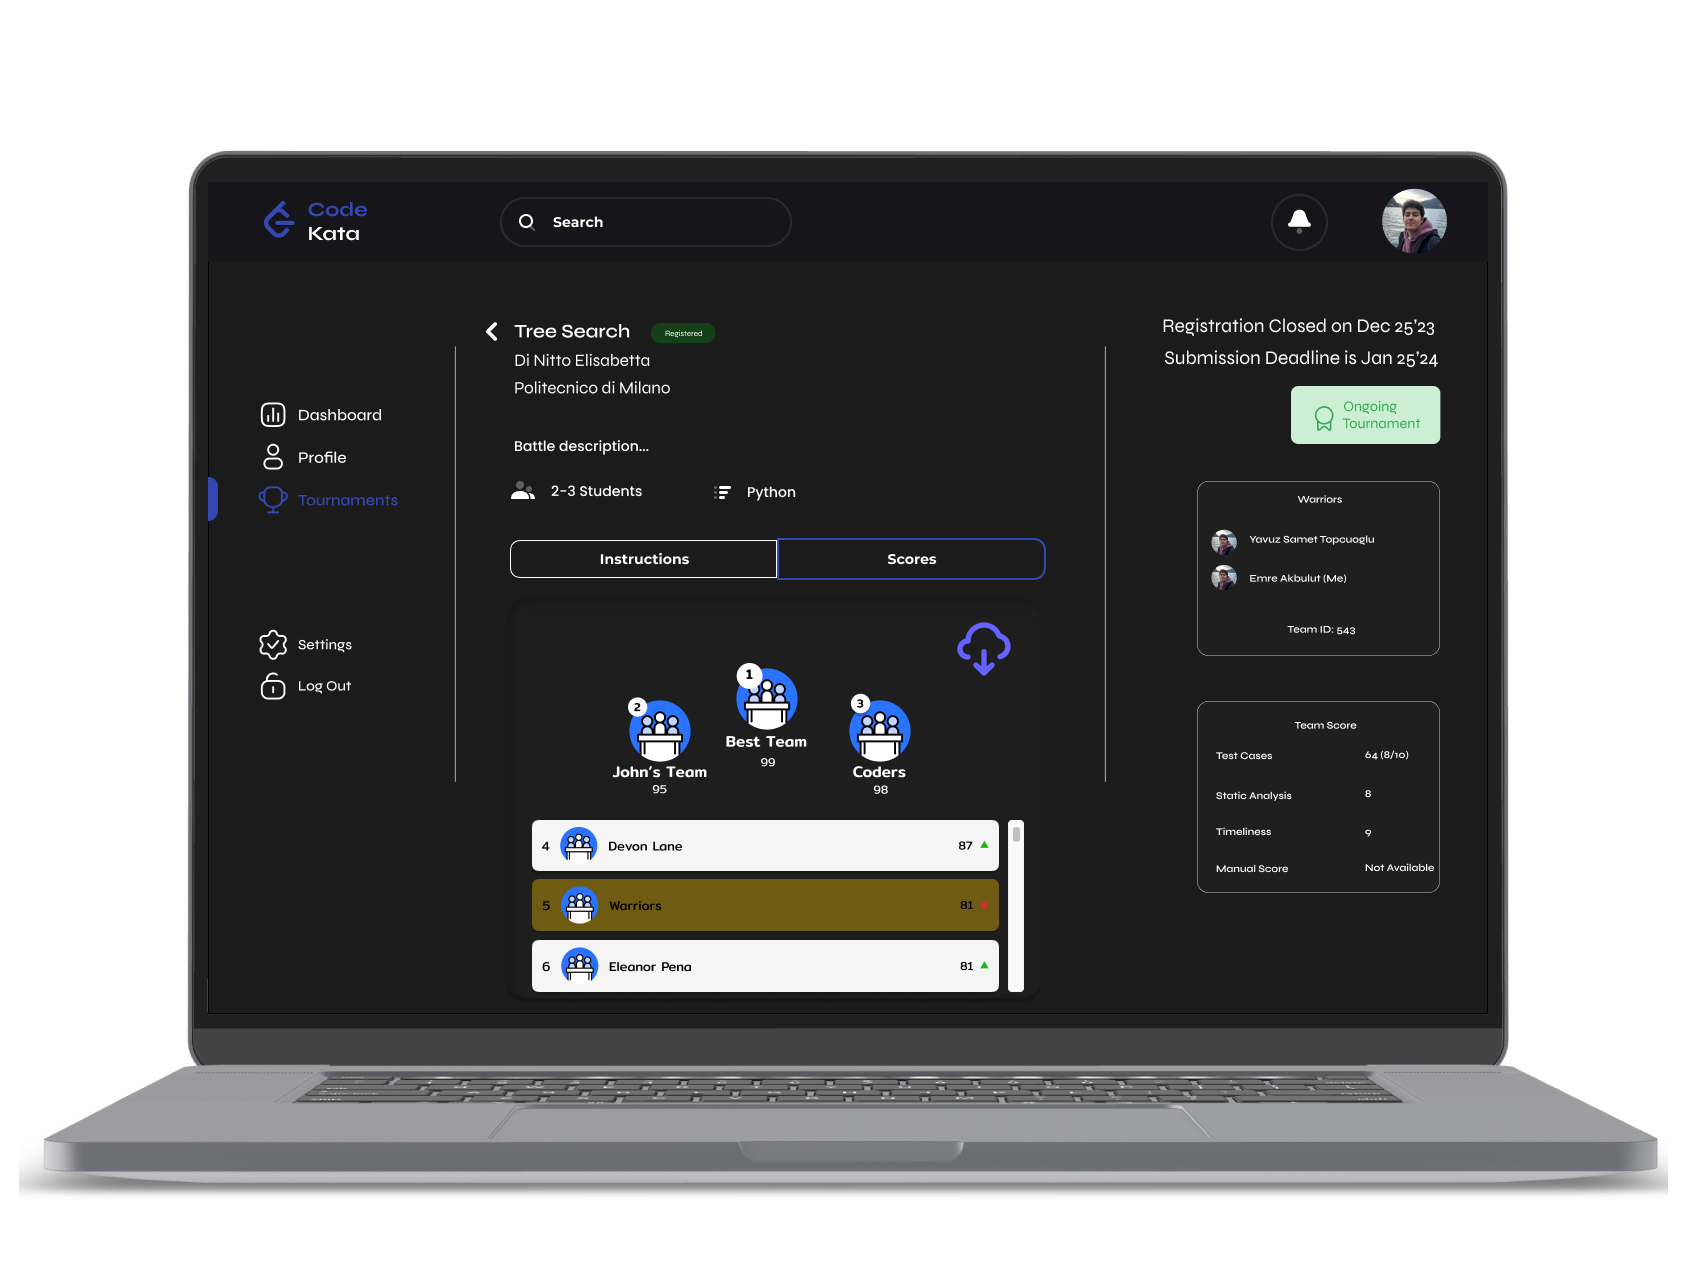
\includegraphics[scale=0.13]{Images/ui-ux/student_battle_4.png}
      (g) $UI_{7}$  Battle Screen for Student
\end{center}

\begin{center}
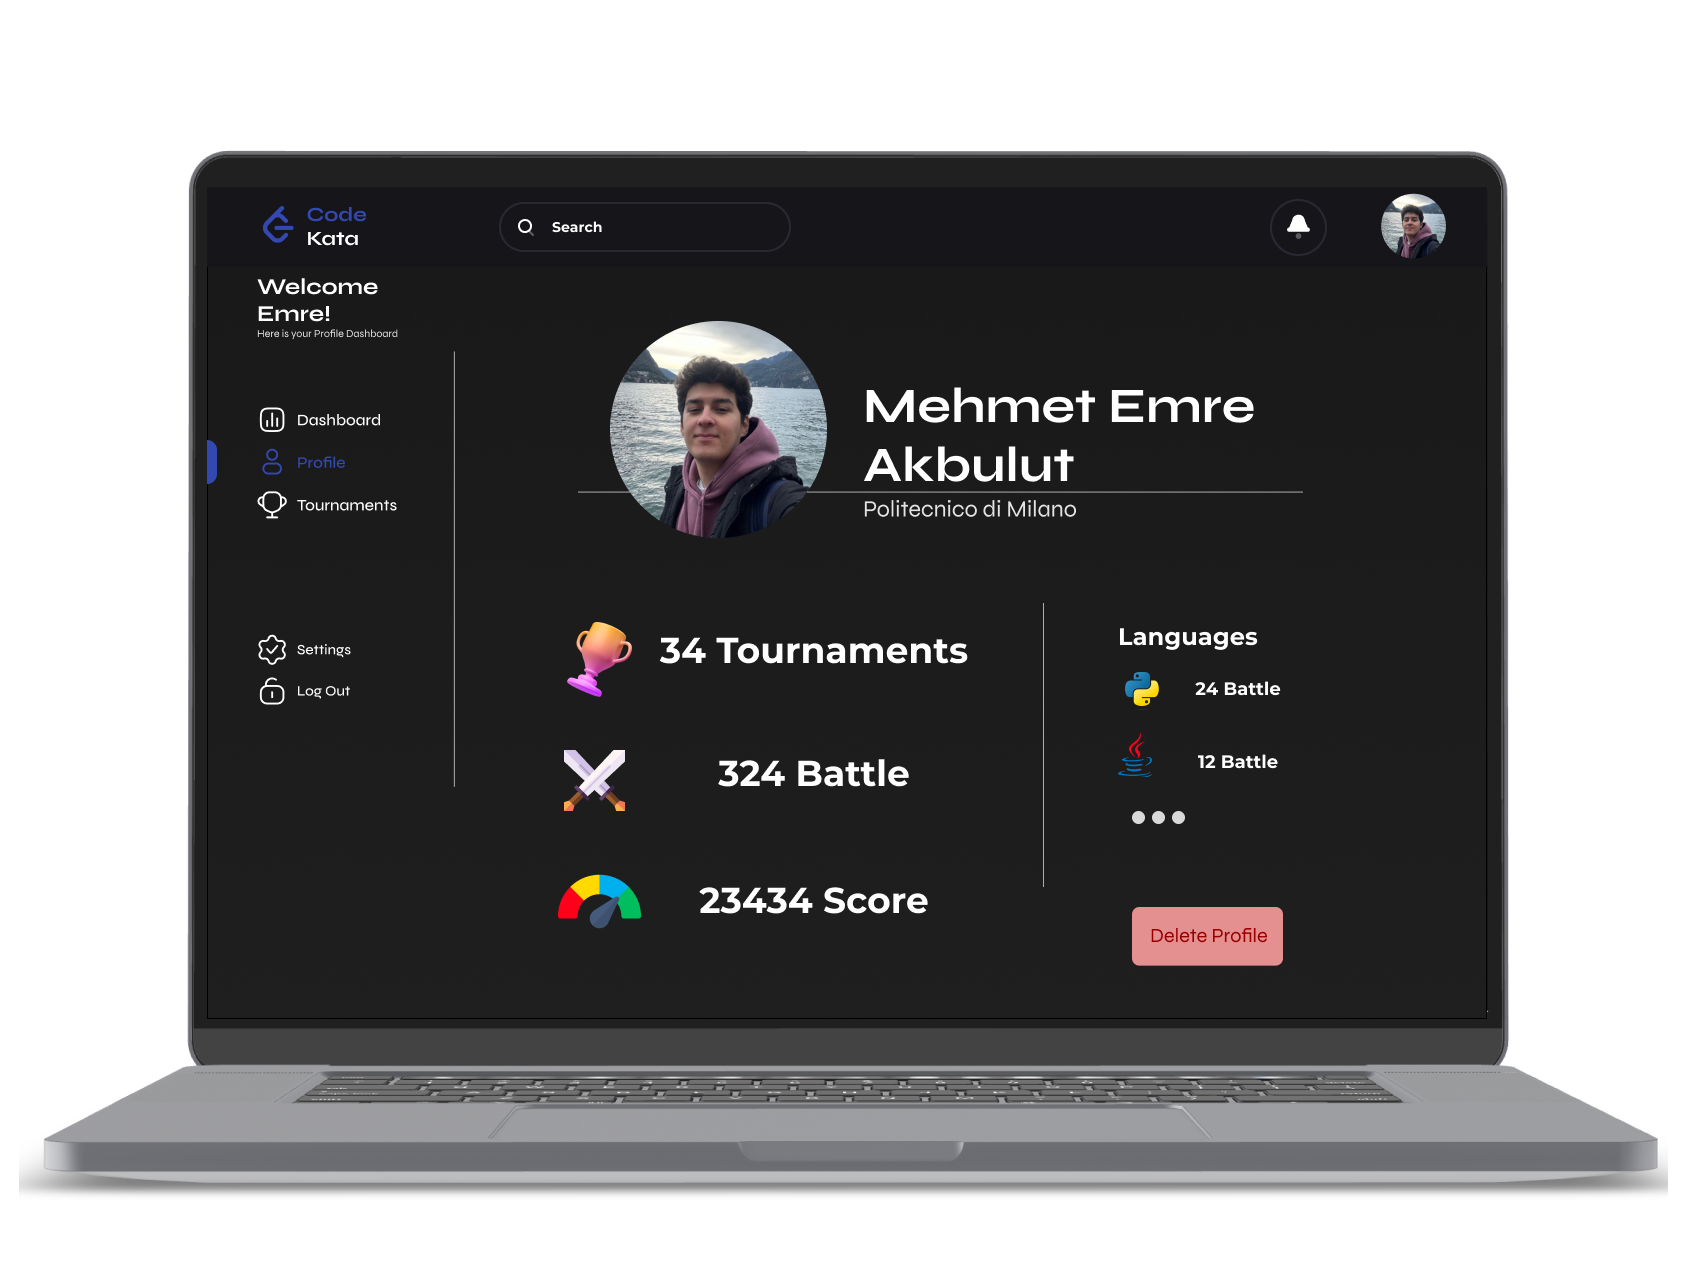
\includegraphics[scale=0.13]{Images/ui-ux/student_profile.png}
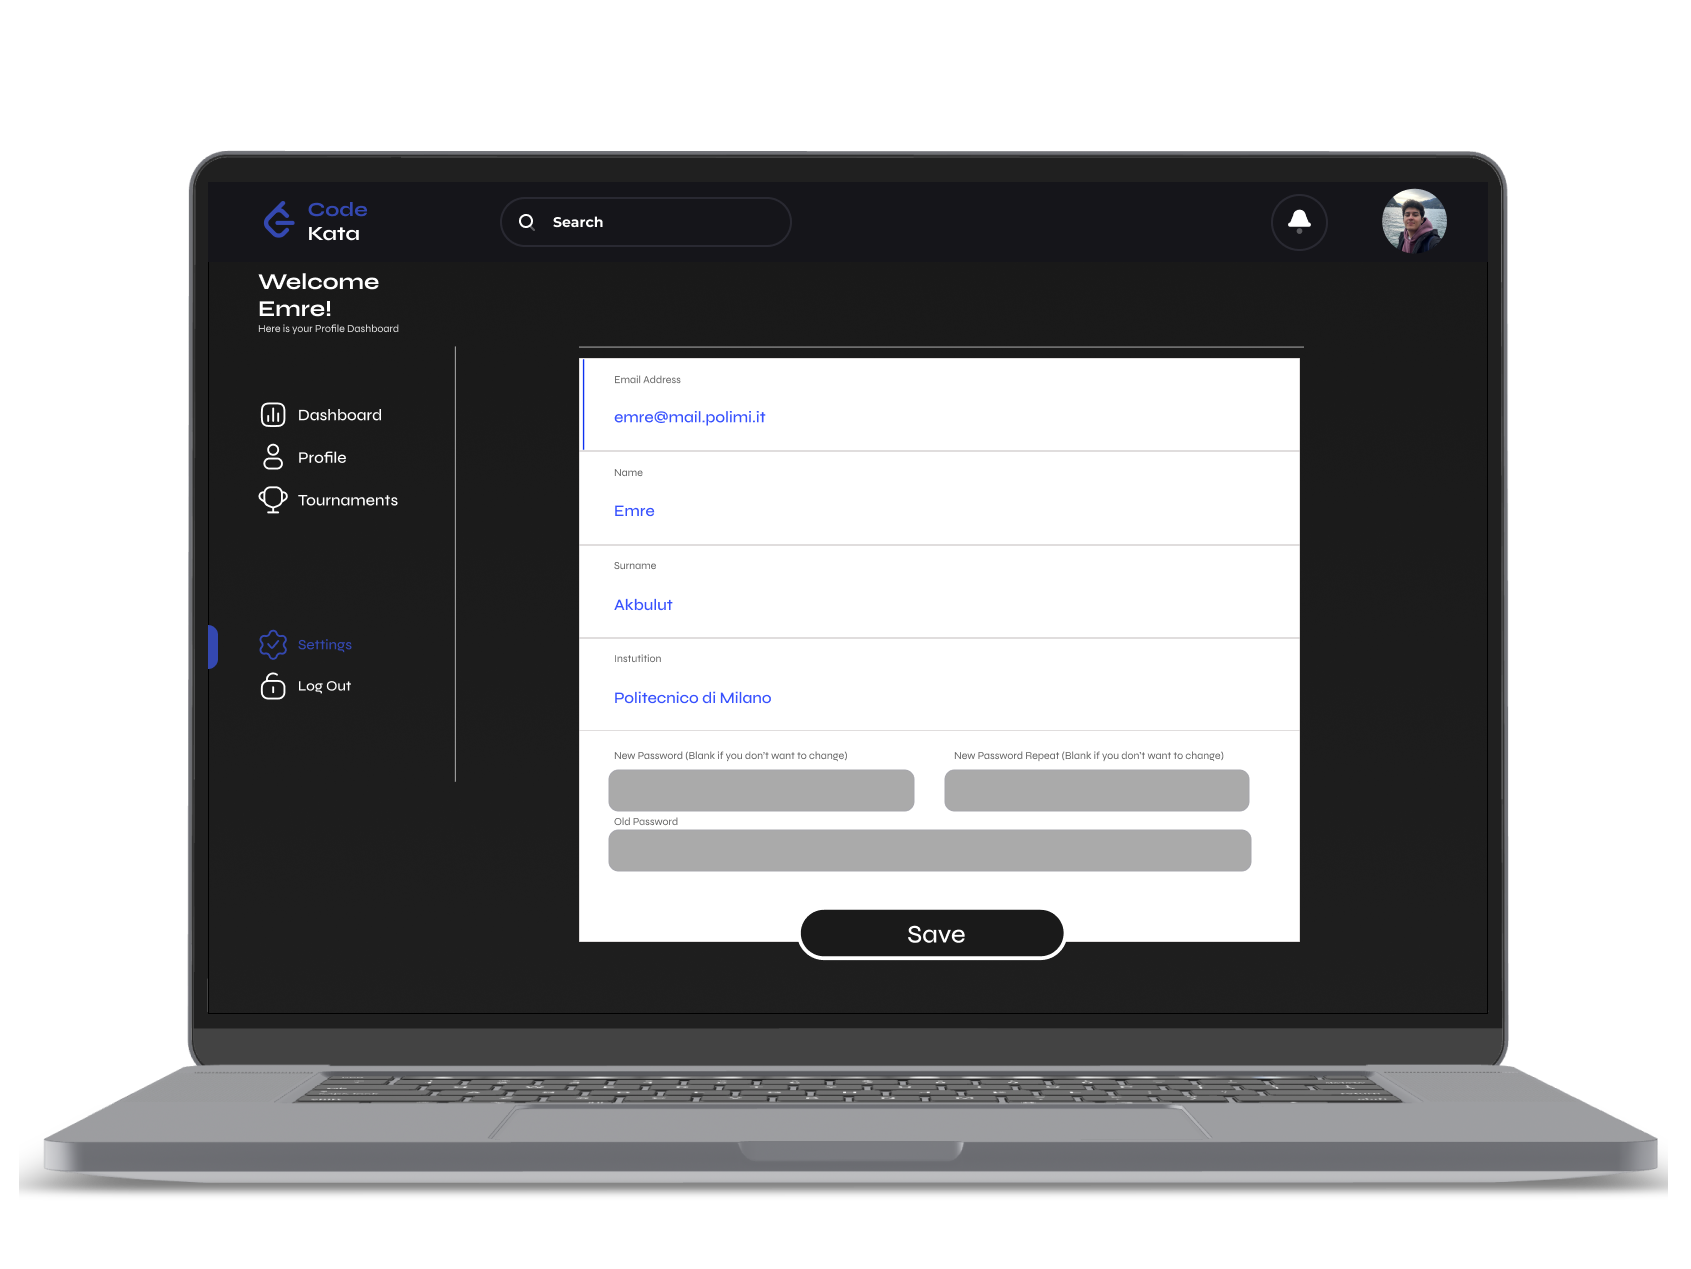
\includegraphics[scale=0.13]{Images/ui-ux/student_settings.png}
        (h) $UI_{8}$  Profile and Settings for Student
\end{center}
\newpage
\begin{center}
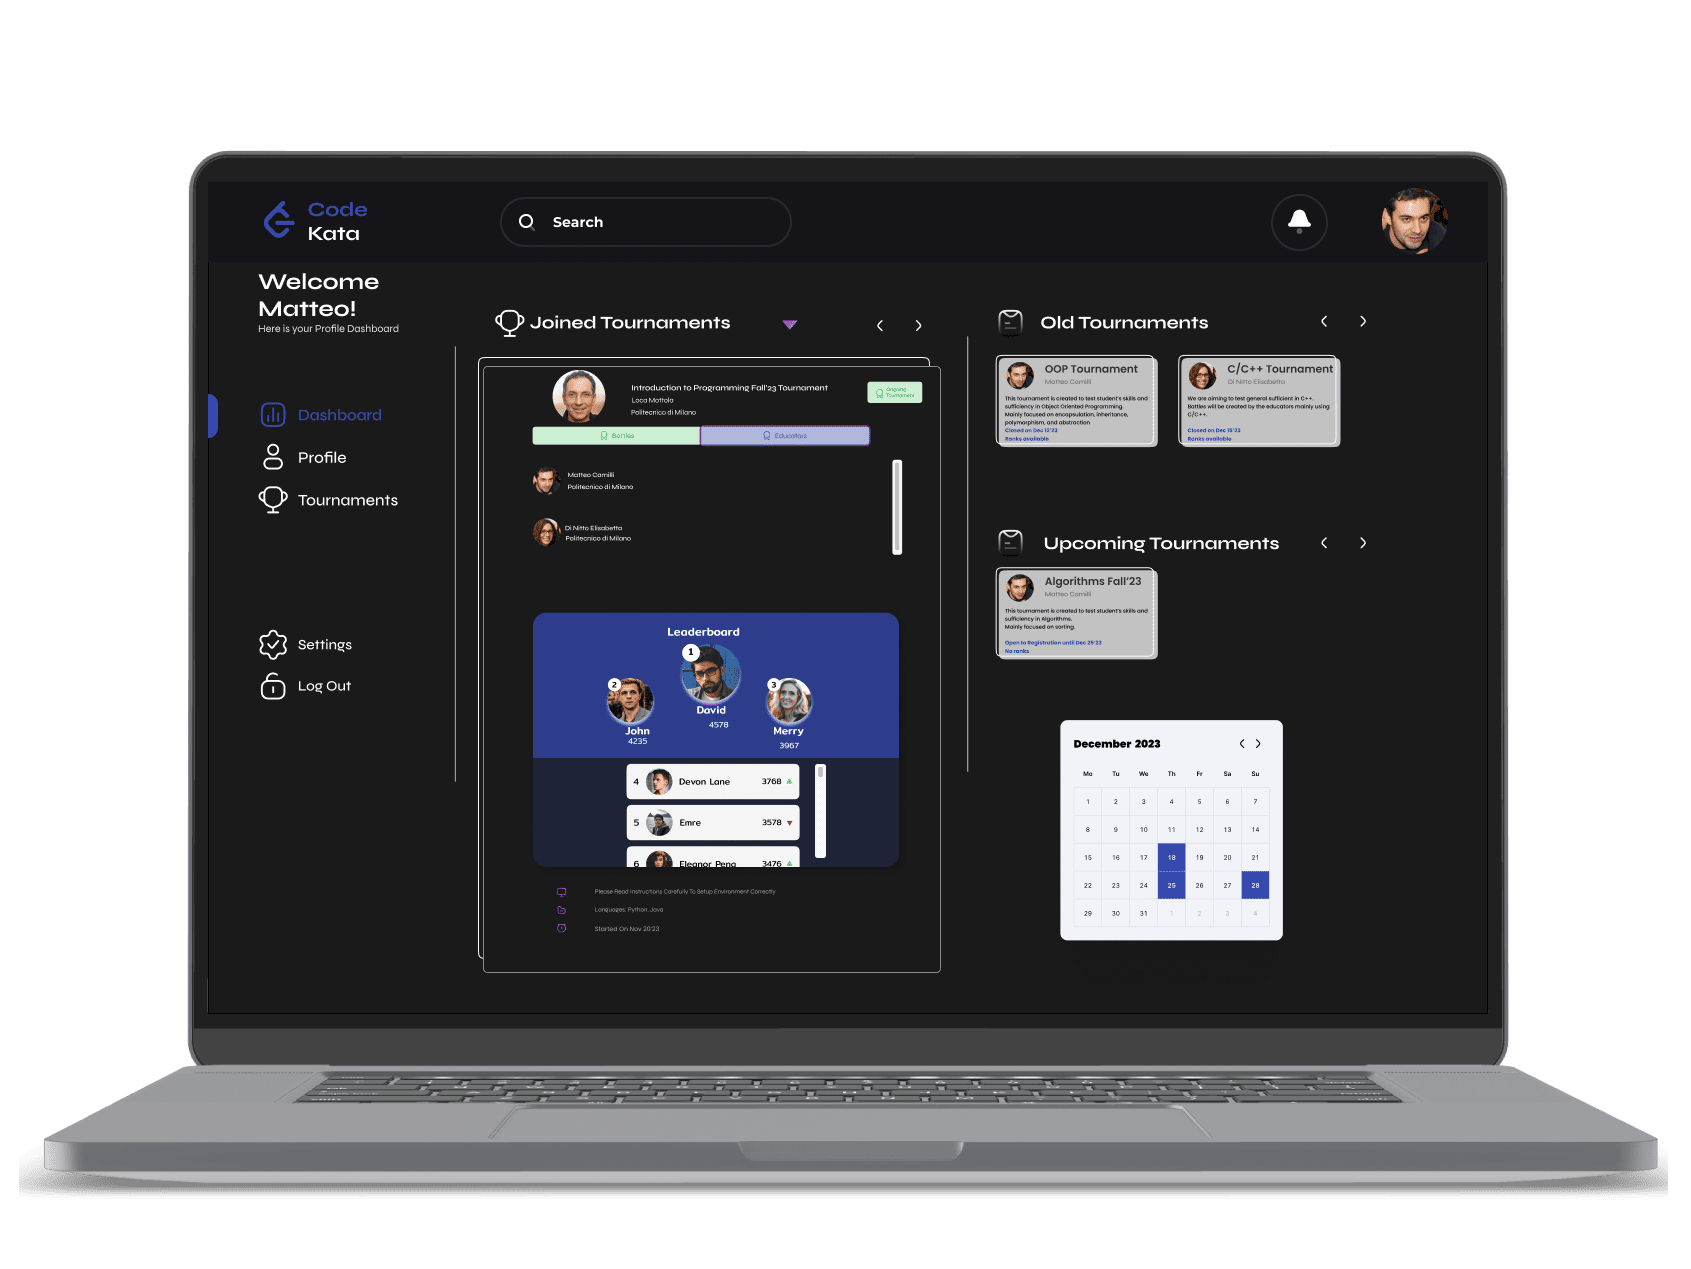
\includegraphics[scale=0.13]{Images/ui-ux/educator_dashboard_1.png}
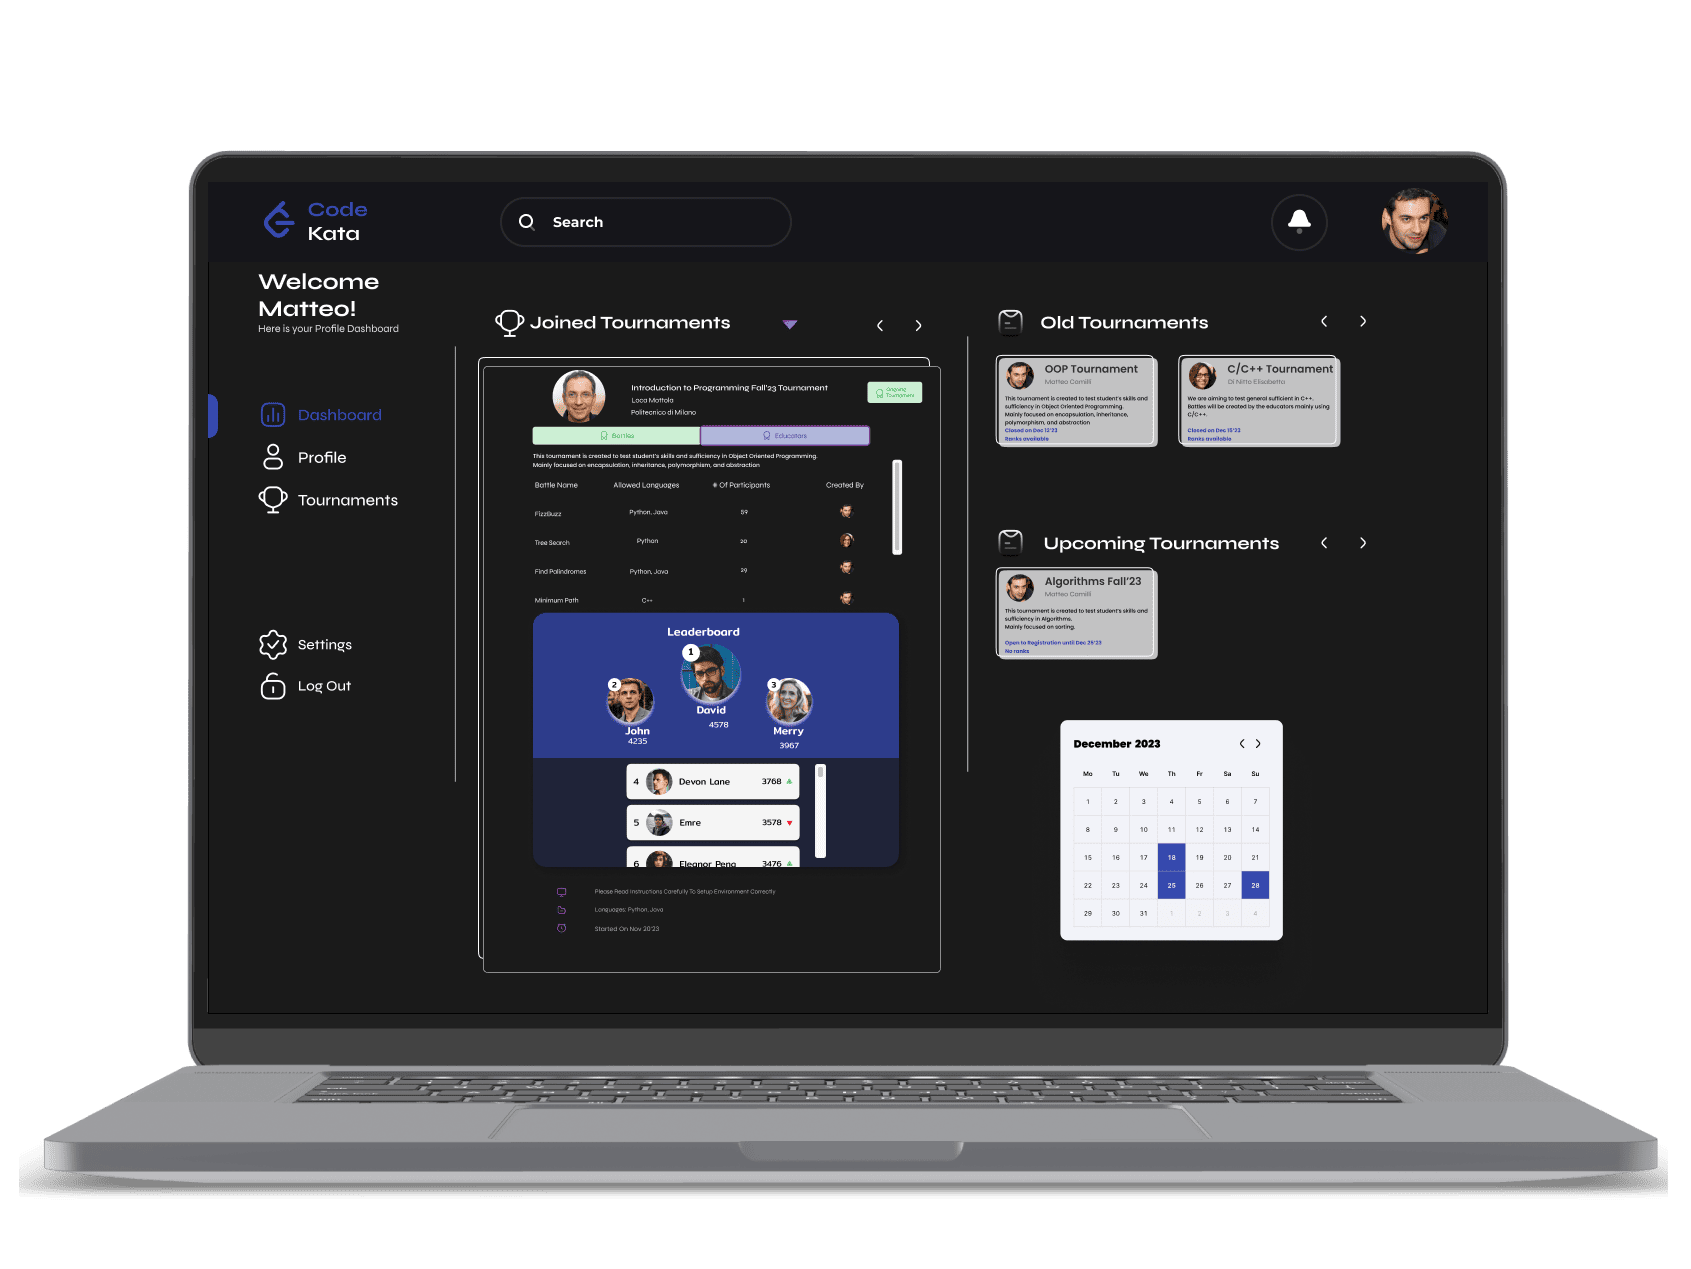
\includegraphics[scale=0.13]{Images/ui-ux/educator_dashboard_2.png}
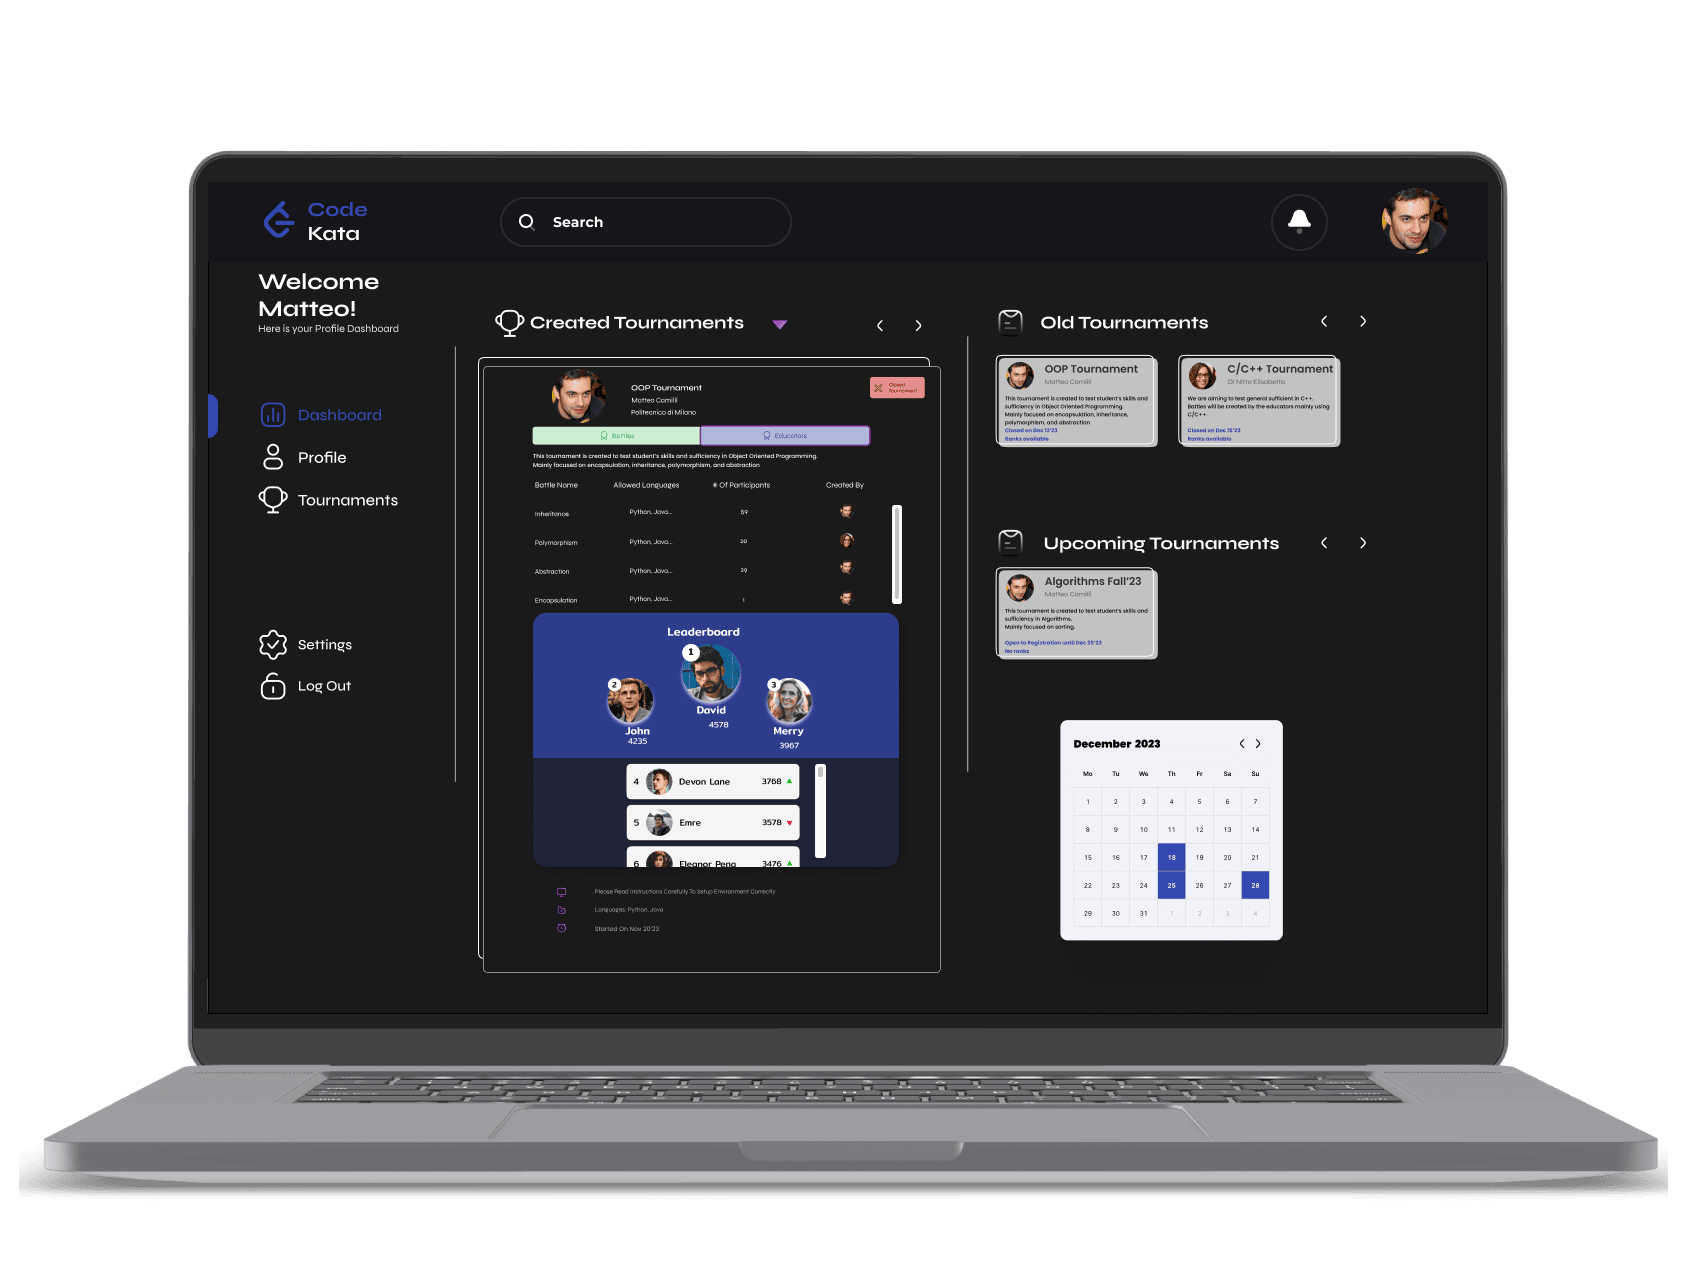
\includegraphics[scale=0.13]{Images/ui-ux/educator_dashboard_3.png}
\\ (i) $UI_{9}$  Educator Dashboard
\end{center}
\begin{center}
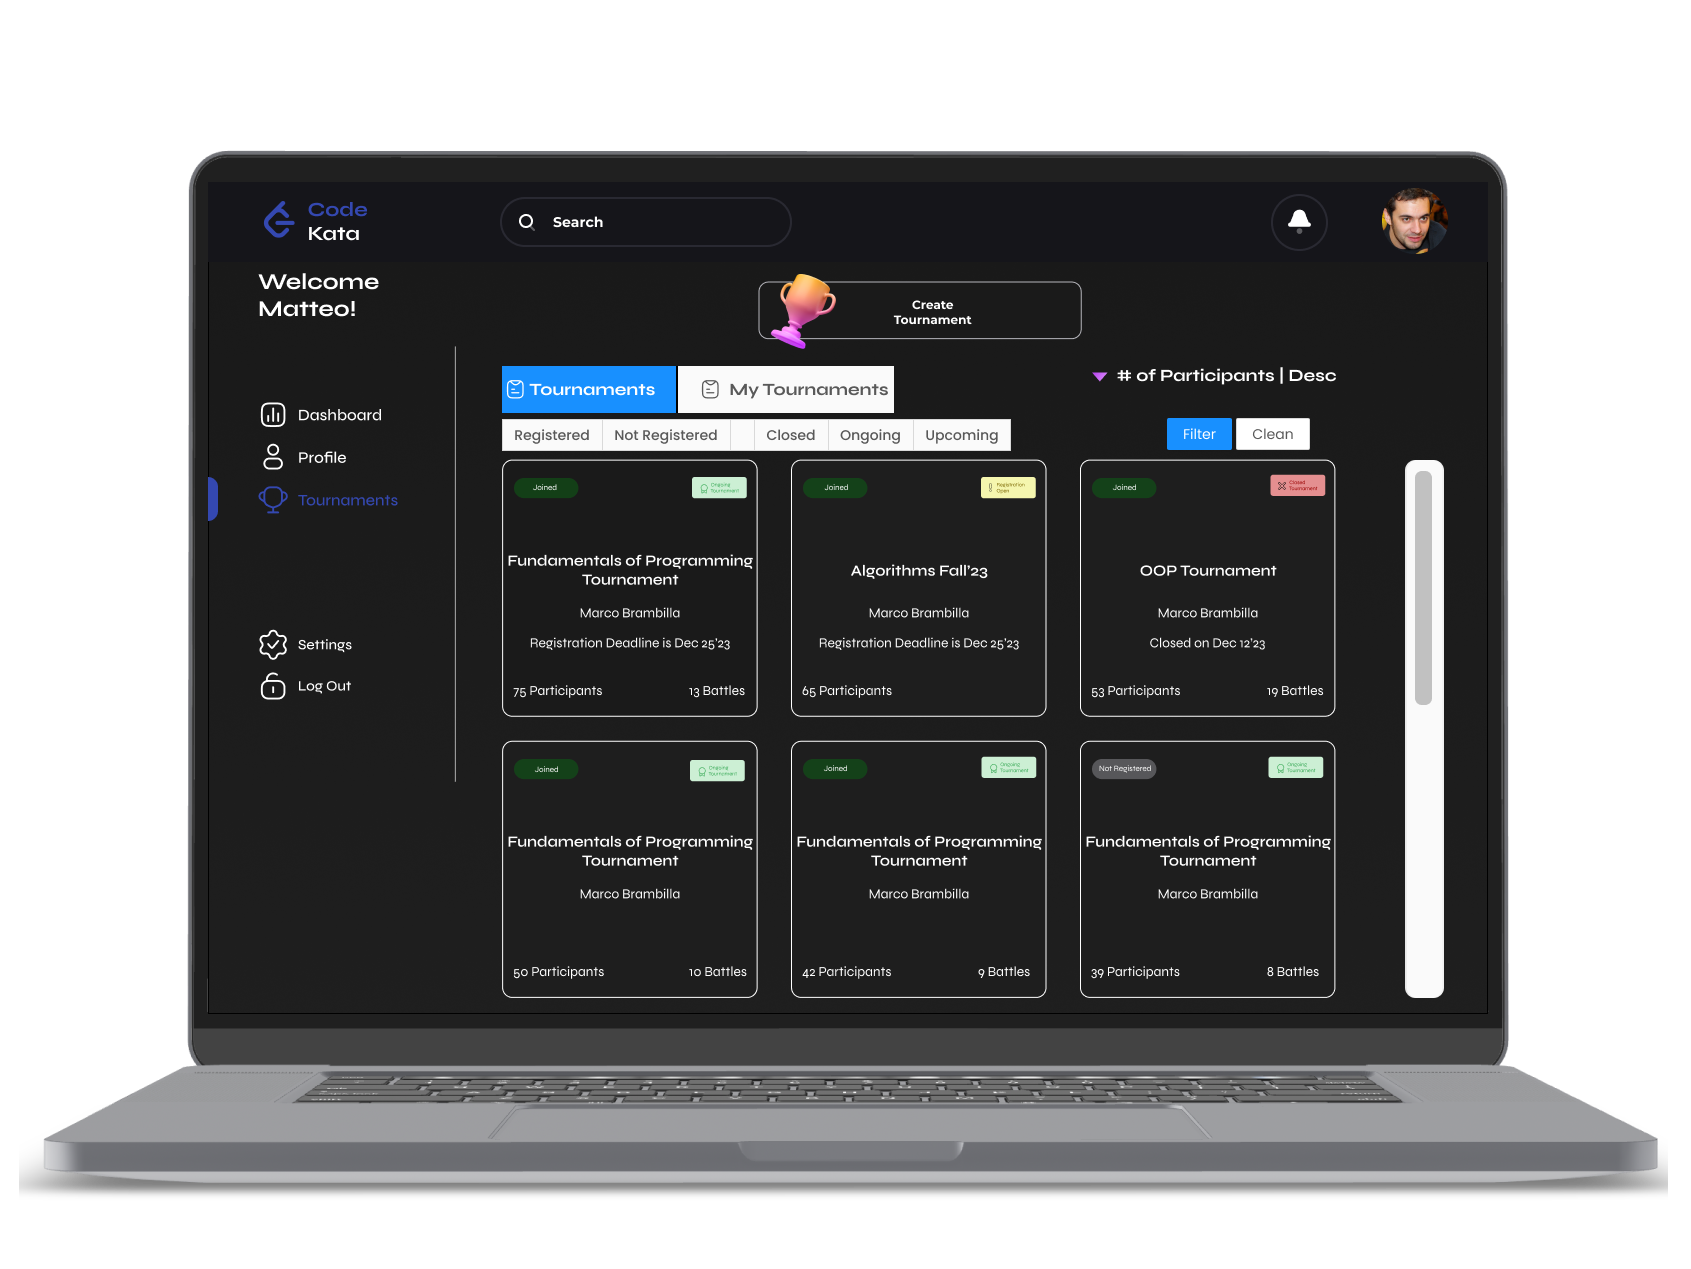
\includegraphics[scale=0.13]{Images/ui-ux/educator_tournaments_1.png}
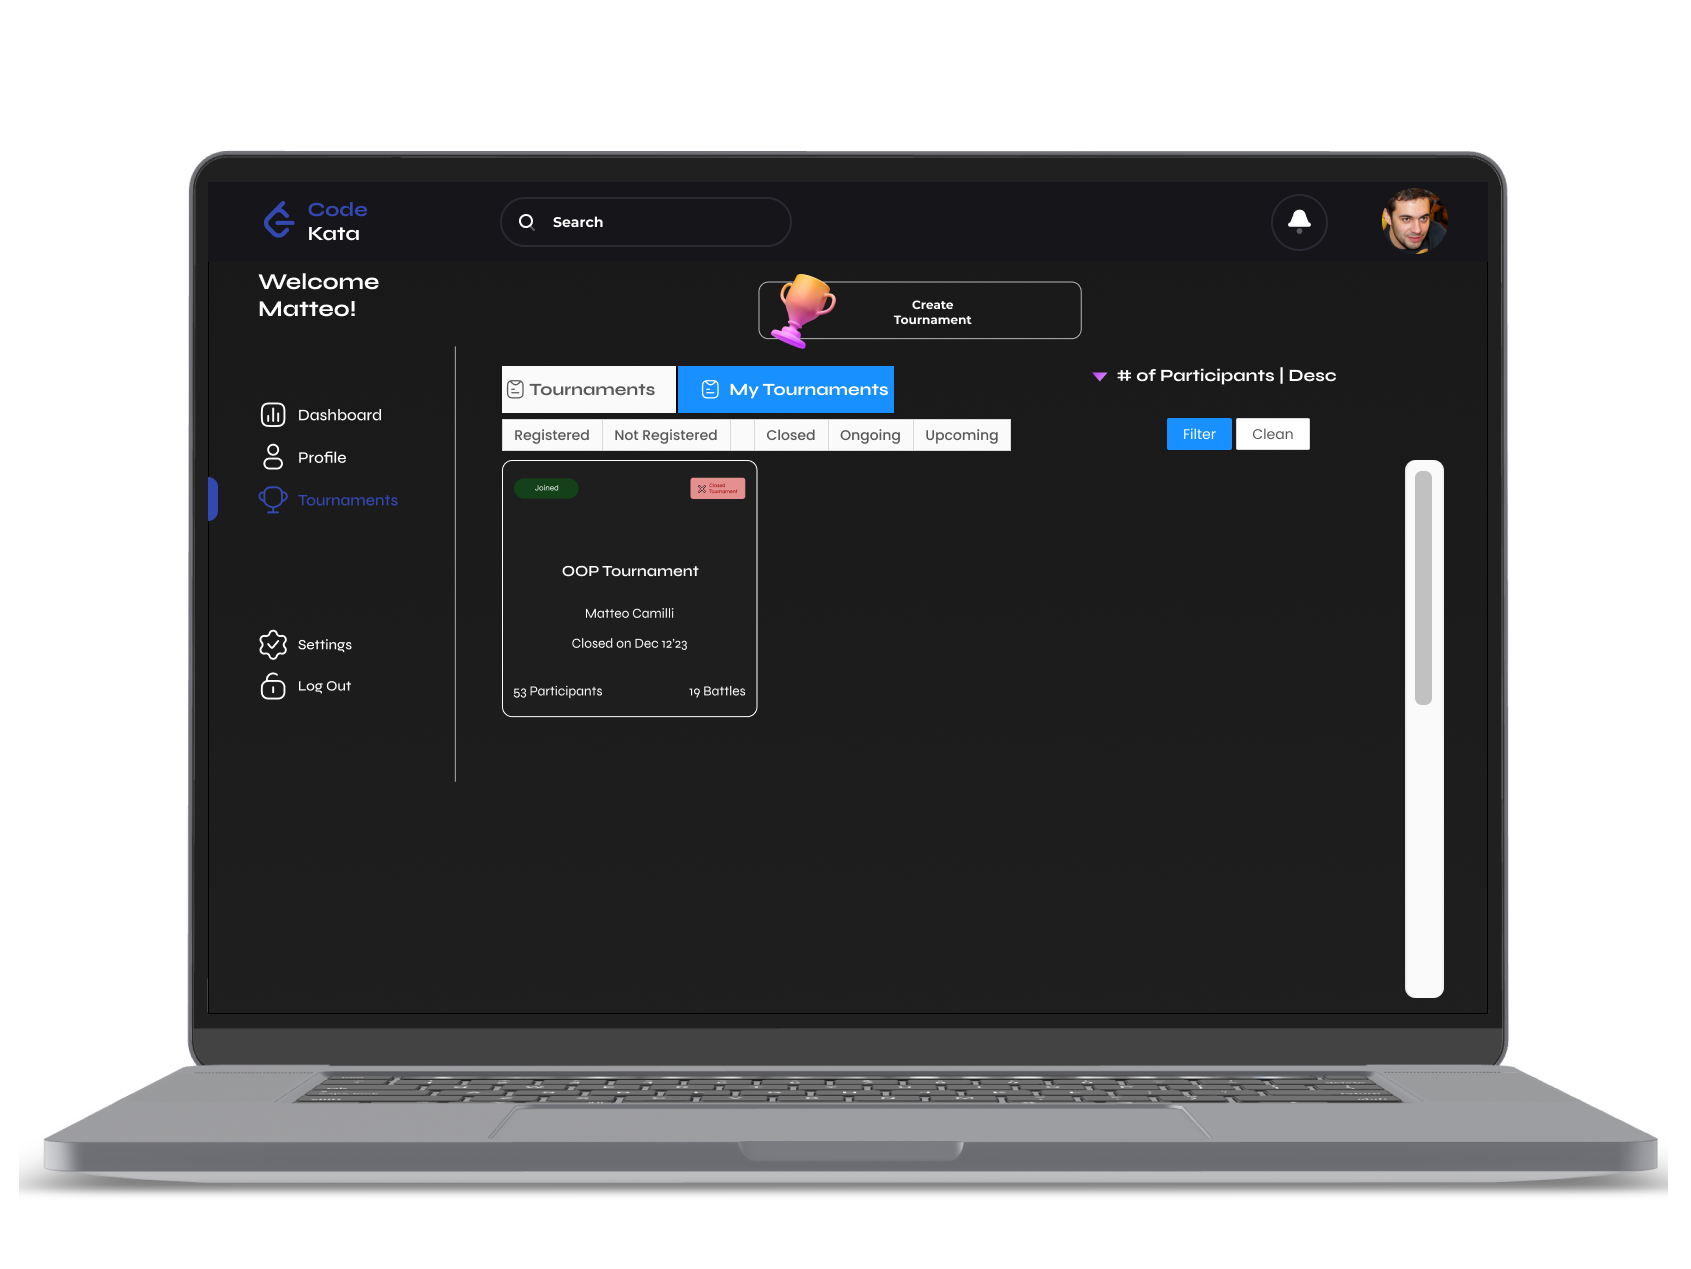
\includegraphics[scale=0.13]{Images/ui-ux/educator_tournaments_2.png}
        (j) $UI_{10}$  Educator Tournaments
\end{center}
\begin{center}
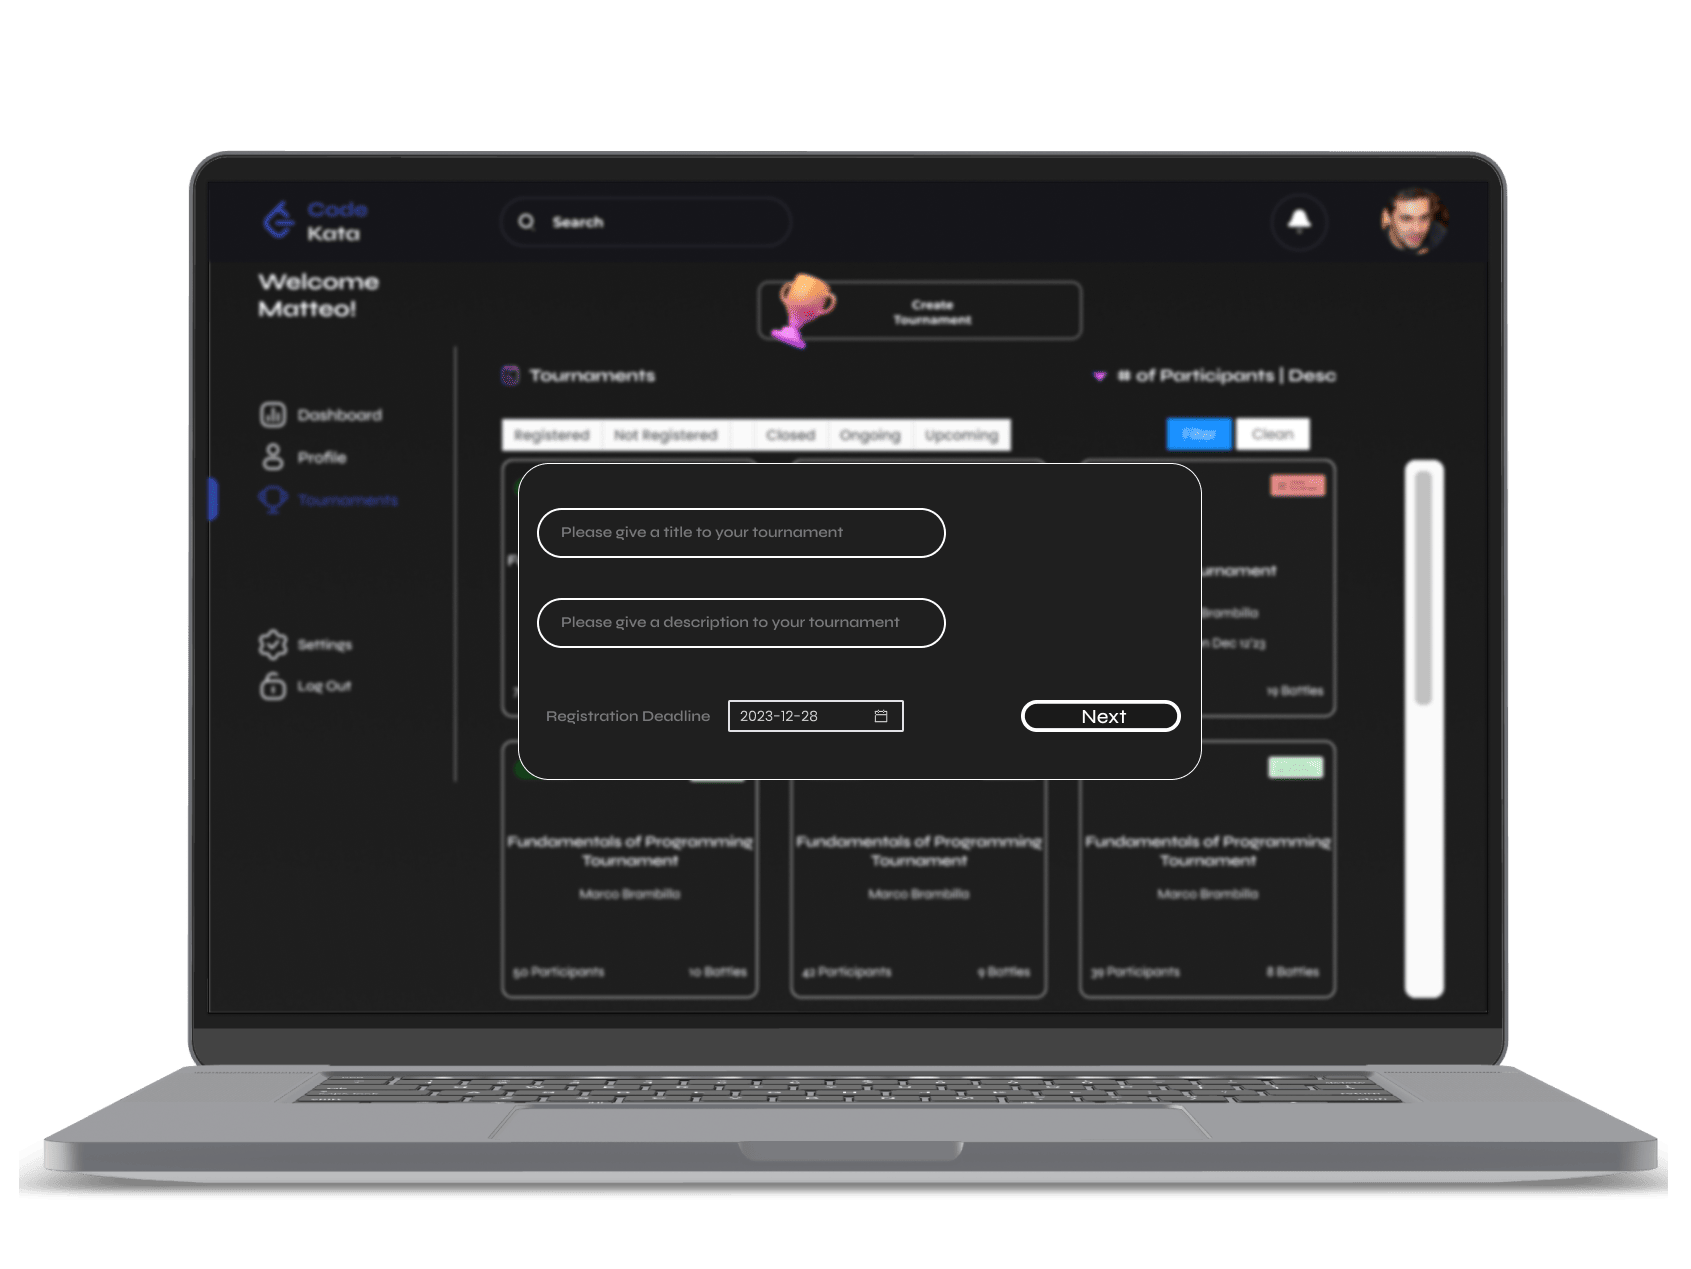
\includegraphics[scale=0.13]{Images/ui-ux/educator_create_tournament_1.png}
\includegraphics[scale=0.13]{Images/ui-ux/educator_create_tournament_2.png}
\includegraphics[scale=0.13]{Images/ui-ux/educator_create_tournament_3.png}
\includegraphics[scale=0.13]{Images/ui-ux/educator_create_tournament_4.png}
        (k) $UI_{11}$ Educator Creates Tournament
\end{center}
\newpage
\begin{center}
\includegraphics[scale=0.13]{Images/ui-ux/educator_creates_battle_1.png}
\includegraphics[scale=0.13]{Images/ui-ux/educator_creates_battle_2.png}
\includegraphics[scale=0.13]{Images/ui-ux/educator_creates_battle_3.png}
\includegraphics[scale=0.13]{Images/ui-ux/educator_creates_battle_4.png}
\includegraphics[scale=0.13]{Images/ui-ux/educator_creates_battle_5.png}
\includegraphics[scale=0.13]{Images/ui-ux/educator_creates_battle_6.png}
        (l) $UI_{12}$ Educator Creates Battle
\end{center}
\newpage
\begin{center}
\includegraphics[scale=0.13]{Images/ui-ux/educator_battle_1.png}
\includegraphics[scale=0.13]{Images/ui-ux/educator_battle_2.png}
\includegraphics[scale=0.13]{Images/ui-ux/educator_battle_3.png}
\\ (m) $UI_{13}$  Educator visits Battle
\end{center}
\newpage
\begin{center}
\includegraphics[scale=0.13]{Images/ui-ux/educator_team_1 (1).png}
\includegraphics[scale=0.13]{Images/ui-ux/educator_team_2 (1).png}
\includegraphics[scale=0.13]{Images/ui-ux/educator_team_3 (1).png}
\includegraphics[scale=0.13]{Images/ui-ux/educator_team_4 (1).png}
        (n) $UI_{14}$  Educator, Team and Manual Scoring
\end{center}
\begin{center}
\includegraphics[scale=0.13]{Images/ui-ux/educator_profile.png}
\includegraphics[scale=0.13]{Images/ui-ux/educator_settings.png}
        (o) $UI_{15}$  Educator Profile and Settings
\end{center}
\newpage
\begin{center}
\includegraphics[scale=0.13]{Images/ui-ux/educator_end_tournament.png}
\includegraphics[scale=0.13]{Images/ui-ux/educator_end_tournament_1.png}
        (p) $UI_{16}$  Educator Ends Tournament
\end{center}

\begin{itemize}
    \item \textbf{$UI_{1}$:} This is a mockup for registration of students and educators. $RW_{1}$ is the related runtime diagram for this mockup.
    \item \textbf{$UI_{2}$:} This is mockup for student and educator login. $RW_{2}$ is the related runtime diagram for this mockup.
    \item \textbf{$UI_{3}$:} These are the screens of the student when it enters the application. This screens is created by fetching tournament with different filters.
    \item \textbf{$UI_{4}$:} These are screens of tournaments from students' perspective. Also these screens are related to  $RW_{3}$. Student can easily navigate among different tournaments.
    \item \textbf{$UI_{5}$:} These are screens of a single tournament from users' perspective. Also these screens are related to  $RW_{3}$. User can easily navigate among battles and leaderboard.
    \item \textbf{$UI_{6}$:} In this screen student register for battle by choosing "register as team" option. The following user interfaces $UI_{7}$ also explain the next steps from this design. Related to $RW_{10}$
    \item \textbf{$UI_{7}$:} This screens shows possible states of a battle screen for a student. Also related to $RW_{4}$ and and $RW_{10}$.
    \item \textbf{$UI_{8}$:} Profile and Setting screens of a student. Related to $RW_{5}$
    \item \textbf{$UI_{9}$:} These are the screens of the educator when it enters the application. This screens is created by fetching tournament with different filters.
    \item \textbf{$UI_{10}$:} These are screens of tournaments from educators' perspective. Also these screens are related to  $RW_{3}$. Educators can easily navigate among different tournaments.
    \item \textbf{$UI_{11}$:} These screens demonstrate the pages for tournament creation. As you can see another educators can be invited. Related to $RW_{6}$ and $RW_{11}$
    \item \textbf{$UI_{12}$:} These screens demonstrate the pages for battle creation. Related to $RW_{6}$ and $RW_{12}$
    \item \textbf{$UI_{13}$:} These screens demonstrate the pages for viewing a battle.  Related to $RW_{4}$
    \item \textbf{$UI_{14}$:} These screen shows how educators can see a submission made by students. Also it demonstrates the manual scoring.
    Related to $RW_{13}$, $RW_{14}$ and $RW_{15}$
    \item \textbf{$UI_{15}$:} Profile and Setting screens of a educator. Related to $RW_{5}$
    \item \textbf{$UI_{16}$:} Educator ends tournament.
\end{itemize}

\newpage


%------------------------------------------------------------------------------------------------------------------------------------------------
\clearpage
{\color{Blue}{\section{Requirements Traceability}}}
\label{sect:reqs}
In this section, we are going to illustrate the mapping of the components introduced in this document on the functional requirements introduced in the RASD. Some closely related requirements are explained together in the tables below.

\begin{table}[h!]
  \centering
  \begin{tabular}{lp{12cm}}
    \hline
    \textbf{R1} & The system shall allow unregistered users to register by providing a unique email, a password, a name, a surname, and institution information. \\
    \hline
    \hline
    \textbf{Authentication Manager} & Gets the client request, and directs it to User Repository. \\
    \textbf{User Repository} &  Creates the user.\\
    \textbf{DBMS} & Saves the user. \\
    \textbf{Notification Manager} &  Triggers Email Manager.\\
    \textbf{Email Manager} &  Sends verification email.\\
    \hline
  \end{tabular}
  \captionof{table}{Mapping on $R_{1}$}
\end{table}

\begin{table}[h!]
  \centering
  \begin{tabular}{lp{12cm}}
    \hline
    \textbf{R2} & The system shall allow users who received a verification email to verify their emails. \\
    \hline
    \hline
    \textbf{Authentication Manager} & Gets the client request, and directs it to User Repository. \\
    \textbf{User Repository} &  Verifies the user.\\
    \textbf{DBMS} & Updates the user. \\
    \hline
  \end{tabular}
  \captionof{table}{Mapping on $R_{2}$}
\end{table}

\begin{table}[h!]
  \centering
  \begin{tabular}{lp{12cm}}
    \hline
    \textbf{R3} & The system shall allow registered users to log in by providing an email, and a password. \\
    \hline
    \hline
    \textbf{Authentication Manager} & Gets the client request, and directs it to User Repository. \\
    \textbf{User Repository} &  Validates the user credentials.\\
    \textbf{DBMS} & Returns user info. \\
    \hline
  \end{tabular}
  \captionof{table}{Mapping on $R_{3}$}
\end{table}

\begin{table}[h!]
  \centering
  \begin{tabular}{lp{12cm}}
    \hline
    \textbf{R4} & The system shall allow authenticated users to view all tournaments. \\
    \hline
    \hline
    \textbf{Tournament Manager} & Gets the client request, and directs it to Tournament Repository. \\
    \textbf{Tournament Repository} &  Gets all tournaments.\\
    \textbf{DBMS} & Returns all tournaments. \\
    \hline
  \end{tabular}
  \captionof{table}{Mapping on $R_{4}$}
\end{table}

\begin{table}[h!]
  \centering
  \begin{tabular}{lp{12cm}}
    \hline
    \textbf{R5} & The system shall allow authenticated users to filter the tournaments by the registration status and availability.  \\
    \hline
    \hline
    \textbf{Tournament Manager} & Gets the client request, and directs it to Tournament Repository. \\
    \textbf{Tournament Repository} &  Gets filtered tournaments using a query.\\
    \textbf{DBMS} & Returns queried tournaments. \\
    \hline
  \end{tabular}
  \captionof{table}{Mapping on $R_{5}$}
\end{table}

\begin{table}[h!]
  \centering
  \begin{tabular}{lp{12cm}}
    \hline
    \textbf{R6} & The system shall allow authenticated users to sort the tournaments by number of participants and number of battles in it. \\
    \hline
    \hline
    \textbf{Tournament Manager} & Gets the client request, and directs it to Tournament Repository. \\
    \textbf{Tournament Repository} &  Gets sorted tournaments using a query.\\
    \textbf{DBMS} & Returns queried tournaments. \\
    \hline
  \end{tabular}
  \captionof{table}{Mapping on $R_{6}$}
\end{table}

\begin{table}[h!]
  \centering
  \begin{tabular}{lp{12cm}}
    \hline
    \textbf{R7} & The system shall allow authenticated users to view a specific tournament. \\
    \hline
    \hline
    \textbf{Tournament Manager} & Gets the client request, and directs it to Tournament Repository. \\
    \textbf{Tournament Repository} &  Gets the tournament by its id using a query.\\
    \textbf{DBMS} & Returns queried tournament. \\
    \hline
  \end{tabular}
  \captionof{table}{Mapping on $R_{7}$}
\end{table}

\begin{table}[h!]
  \centering
  \begin{tabular}{lp{12cm}}
    \hline
    \textbf{R8} & The system shall allow authenticated users to view the leaderboard of the tournament. \\
    \hline
    \hline
    \textbf{Tournament Manager} & Gets the client request, and directs it to Tournament Repository. \\
    \textbf{Tournament Repository} &  Gets the tournament scores of subscribed users and then sorts them.\\
    \textbf{DBMS} & Returns tournament scores. \\
    \hline
  \end{tabular}
  \captionof{table}{Mapping on $R_{8}$}
\end{table}

\begin{table}[h!]
  \centering
  \begin{tabular}{lp{12cm}}
    \hline
    \textbf{R9} & The system shall allow authenticated users to view all battles in a tournament. \\
    \hline
    \hline
    \textbf{Tournament Manager} & Gets the client request, and directs it to Tournament Repository. \\
    \textbf{Tournament Repository} &  Gets the list of battles of the tournament.\\
    \textbf{DBMS} & Returns the list of battles. \\
    \hline
  \end{tabular}
  \captionof{table}{Mapping on $R_{9}$}
\end{table}

\begin{table}[h!]
  \centering
  \begin{tabular}{lp{12cm}}
    \hline
    \textbf{R10} & The system shall allow authenticated users to filter the battles by group size, start date - end date, registration status, institution of the battle creator, allowed programming languages, and the battle creator. \\
    \hline
    \hline
    \textbf{Battle Manager} & Gets the client request, and directs it to Battle Repository. \\
    \textbf{Battle Repository} &  Gets filtered battles using a query.\\
    \textbf{DBMS} & Returns queried battles. \\
    \hline
  \end{tabular}
  \captionof{table}{Mapping on $R_{10}$}
\end{table}

\begin{table}[h!]
  \centering
  \begin{tabular}{lp{12cm}}
    \hline
    \textbf{R11} & The system shall allow authenticated users to search battles by text search. \\
    \hline
    \hline
    \textbf{Battle Manager} & Gets the client request, and directs it to Battle Repository. \\
    \textbf{Battle Repository} &  Gets searched battles using a query.\\
    \textbf{DBMS} & Returns queried battles. \\
    \hline
  \end{tabular}
  \captionof{table}{Mapping on $R_{11}$}
\end{table}

\begin{table}[h!]
  \centering
  \begin{tabular}{lp{12cm}}
    \hline
    \textbf{R12} & The system shall allow authenticated users to view a specific battle and its instructions. \\
    \hline
    \hline
    \textbf{Battle Manager} & Gets the client request, and directs it to Battle Repository. \\
    \textbf{Battle Repository} &   Gets the battle by its id using a query.\\
    \textbf{DBMS} & Returns queried battle. \\
    \hline
  \end{tabular}
  \captionof{table}{Mapping on $R_{12}$}
\end{table}

\begin{table}[h!]
  \centering
  \begin{tabular}{lp{12cm}}
    \hline
    \textbf{R13} & The system shall allow authenticated users to view the rankings of the battle. \\
    \hline
    \hline
    \textbf{Battle Manager} & Gets the client request, and directs it to Battle Repository. \\
    \textbf{Battle Repository} & Gets the battle scores of participating teams and then sorts them.\\
    \textbf{DBMS} & Returns battle scores. \\
    \hline
  \end{tabular}
  \captionof{table}{Mapping on $R_{13}$}
\end{table}

\begin{table}[h!]
  \centering
  \begin{tabular}{lp{12cm}}
    \hline
    \textbf{R14} & The system shall allow authenticated users to search tournaments with text search by educators, by titles, or by institutions.\\
    \hline
    \hline
    \textbf{Tournament Manager} & Gets the client request, and directs it to Tournament Repository. \\
    \textbf{Tournament Repository} & Gets searched tournaments using a query.\\
    \textbf{DBMS} & Returns queried tournaments. \\
    \hline
  \end{tabular}
  \captionof{table}{Mapping on $R_{14}$}
\end{table}

\begin{table}[h!]
  \centering
  \begin{tabular}{lp{12cm}}
    \hline
    \textbf{R15} & The system shall allow authenticated users to manage their profiles.
  \begin{enumerate}[(a)]
      \item The system shall allow authenticated users to view their profiles.
      
  \item The system shall allow authenticated users to delete their profiles unless they do not have an ongoing tournament created by themselves.

    \item The system shall allow authenticated users to view their settings.
  \item The system shall allow authenticated users to edit their settings by name, surname, password, and institution information.
  \item The system shall oblige authenticated users to enter their old password during settings editing.
  
      
  \end{enumerate}
\\
    \hline
    \hline
    \textbf{Profile Manager} & Gets the client request, and directs it to User Repository. \\
    \textbf{User Repository} & \begin{enumerate}[(a)]
      \item Gets the user profile.
      
  \item Deletes the user.
    \item Gets the user settings.
  \item Edits the user settings.
  \item Edits the user settings.
  
      
  \end{enumerate}
    
    \\
    \textbf{DBMS} & \begin{enumerate}[(a)]
      \item Returns user profile.
      
  \item Removes user.

    \item Returns user settings.
  \item Updates user settings.
\item Updates user settings.
  
      
  \end{enumerate}
    
    
    
    \\
    \hline
  \end{tabular}
  \captionof{table}{Mapping on $R_{15}$}
\end{table}



\begin{table}[h!]
  \centering
  \begin{tabular}{lp{12cm}}
    \hline
    \textbf{R16} & The system shall allow educators to create tournaments by providing a title, a description, and a registration 
    deadline. \\
    \textbf{R34} & The system shall trigger the email service to send a notification email for a newly created tournament for all registered users.\\
    \hline
    \hline
    \textbf{Tournament Manager} & Gets the client request, and directs it to Tournament Repository. \\
    \textbf{Tournament Repository} & Creates the tournament.\\
    \textbf{DBMS} & Saves the tournament. \\
    \textbf{Notification Manager} &  Triggers Email Manager.\\
    \textbf{Email Manager} &  Sends notification email to all users.\\
    \hline
  \end{tabular}
  \captionof{table}{Mapping on $R_{16}$ and $R_{34}$}
\end{table}


\begin{table}[h!]
  \centering
  \begin{tabular}{lp{12cm}}
    \hline
    \textbf{R17} & The system shall allow educators to invite other educators to their tournaments during tournament creation. \\
    \textbf{R37} & The system shall trigger the email service to send an invitation notification for the tournament to the invitee educators.\\
    \hline
    \hline
    \textbf{Tournament Manager} & Gets the client request, and directs it to Tournament Repository. \\
    \textbf{Tournament Repository} & Creates the tournament.\\
    \textbf{DBMS} & Saves the tournament. \\
    \textbf{Notification Manager} &  Triggers In-App Notification Manager.\\
    \textbf{In-App Notification Manager} &  Sends invitation notification to invitee educators.\\
    \hline
  \end{tabular}
  \captionof{table}{Mapping on $R_{17}$ and $R_{37}$}
\end{table}

\begin{table}[h!]
  \centering
  \begin{tabular}{lp{12cm}}
    \hline
    \textbf{R18} & The system shall allow educators to edit the tournaments that they have created by providing a title, a description, and a registration deadline unless the registration deadline has not passed. \\
    \hline
    \hline
    \textbf{Tournament Manager} & Gets the client request, and directs it to Tournament Repository. \\
    \textbf{Tournament Repository} & Edits the tournament.\\
    \textbf{DBMS} & Updates the tournament. \\
    \hline
  \end{tabular}
  \captionof{table}{Mapping on $R_{18}$}
\end{table}

\begin{table}[h!]
  \centering
  \begin{tabular}{lp{12cm}}
    \hline
    \textbf{R19} & The system shall allow educators to end the tournaments that they have created. \\
    \hline
    \hline
    \textbf{Tournament Manager} & Gets the client request, and directs it to Tournament Repository. \\
    \textbf{Tournament Repository} & Ends the tournament.\\
    \textbf{DBMS} & Updates the tournament. \\
    \hline
  \end{tabular}
  \captionof{table}{Mapping on $R_{19}$}
\end{table}

\begin{table}[h!]
  \centering
  \begin{tabular}{lp{12cm}}
    \hline
    \textbf{R20} & The system shall allow educators to accept or reject the tournament invitation to create battles coming from other educators for a tournament. \\
    \hline
    \hline
    \textbf{Tournament Manager} & Gets the client request, and directs it to Tournament Repository. \\
    \textbf{Tournament Repository} & Adds the educator to the tournament contributors list.\\
    \textbf{DBMS} & Updates the tournament. \\
    \hline
  \end{tabular}
  \captionof{table}{Mapping on $R_{20}$}
\end{table}


\begin{table}[h!]
  \centering
  \begin{tabular}{lp{12cm}}
    \hline
    \textbf{R21} & The system shall allow educators to create battles by providing a title, a description, a registration deadline, a submission deadline, the allowed languages, test cases, build scripts, minimum \& maximum group size, and the scoring criteria. \\
    \hline
    \hline
    \textbf{Battle Manager} & Gets the client request, and directs it to Battle Repository. \\
    \textbf{Battle Repository} & Creates the battle.\\
    \textbf{DBMS} & Saves the battle. \\
    \textbf{Notification Manager} &  Triggers Email Manager.\\
    \textbf{Email Manager} &  Sends notification email to users that subscribe to the battle's tournament.\\
    \hline
  \end{tabular}
  \captionof{table}{Mapping on $R_{21}$}
\end{table}


\begin{table}[h!]
  \centering
  \begin{tabular}{lp{12cm}}
    \hline
    \textbf{R22} & The system shall oblige educators to upload test case file and build script for every allowed language in battle. \\
    \hline
    \hline
    \textbf{Battle Manager} & Gets the client request, and uploads the battle files. \\
    \textbf{File Manager} & Stores the battle files. \\
    \hline
  \end{tabular}
  \captionof{table}{Mapping on $R_{22}$}
\end{table}

\begin{table}[h!]
  \centering
  \begin{tabular}{lp{12cm}}
    \hline
    \textbf{R23} & The system shall allow educators to manually evaluate the submissions giving extra point between 0 and 10 after the submission deadline has passed. \\
    \hline
    \hline
    \textbf{Battle Manager} & Gets the client request, and directs it to Submission Manager. \\
    \textbf{Submission Manager} & Utilises Scoring Manager, and gives the score to the Submission Repository.\\
    \textbf{Scoring Manager} & Enables educator to evaluate. \\
     \textbf{Submission Repository} & Gives point to the submission.\\
     \textbf{DBMS} & Updates the submission. \\
    \hline
  \end{tabular}
  \captionof{table}{Mapping on $R_{23}$}
\end{table}

\begin{table}[h!]
  \centering
  \begin{tabular}{lp{12cm}}
    \hline
    \textbf{R24} & The system shall allow educators to edit the battles that they have created. \\
    \hline
    \hline
     \textbf{Battle Manager} & Gets the client request, and directs it to Battle Repository. \\
    \textbf{Battle Repository} & Edits the battle.\\
    \textbf{DBMS} & Updates the battle. \\
    \hline
  \end{tabular}
  \captionof{table}{Mapping on $R_{24}$}
\end{table}

\begin{table}[h!]
  \centering
  \begin{tabular}{lp{12cm}}
    \hline
    \textbf{R25} &  The system shall allow students to register for tournaments. \\
    \hline
    \hline
     \textbf{Tournament Manager} & Gets the client request, and directs it to Tournament Repository. \\
    \textbf{Tournament Repository} & Adds the student to the tournament subscribers.\\
    \textbf{DBMS} & Updates the tournament. \\
    \hline
  \end{tabular}
  \captionof{table}{Mapping on $R_{25}$}
\end{table}


\begin{table}[h!]
  \centering
  \begin{tabular}{lp{12cm}}
    \hline
    \textbf{R26} &  The system shall allow students to register for battles in which the tournaments that they have registered for.\\
    \textbf{R27} &  The system shall allow students to register for battles individually.\\
    \textbf{R28} &  The system shall allow students to register for battles by a team having a team name.\\
    \hline
    \hline
    \textbf{Battle Manager} & Gets the client request, and triggers Team Manager. With the response coming from the Team Manager, it utilises Battle Repository.\\
    \textbf{Team Manager} & Creates a team. (Regardless of the number of students on the team, it is created. Individual students will be considered as a team of one in the project.)\\
    \textbf{Team Repository} & Creates the team.\\
    \textbf{Battle Repository} & Adds the team to the battle participants.\\
    \textbf{DBMS} & Saves the team, and updates the battle. \\
    \hline
  \end{tabular}
  \captionof{table}{Mapping on $R_{26}$, $R_{27}$, $R_{28}$}
\end{table}

\begin{table}[h!]
  \centering
  \begin{tabular}{lp{12cm}}
    \hline
    \textbf{R29} &  The system shall allow students to invite other students to their team during battle registration. \\
    \textbf{R35} &  The system shall trigger the email service to send an invitation notification for the battle to the invitee students. \\
    \hline
    \hline
    \textbf{Battle Manager} & Gets the client request, and directs it to Team Manager. \\
    \textbf{Team Manager} & Notifies invitee students.\\
    \textbf{Notification Manager} &  Triggers In-App Notification Manager.\\
    \textbf{In-App Notification Manager} &  Sends invitation notification to invitee students.\\
    \hline
  \end{tabular}
  \captionof{table}{Mapping on $R_{29}$}
\end{table}

\begin{table}[h!]
  \centering
  \begin{tabular}{lp{12cm}}
    \hline
    \textbf{R30} &  The system shall allow students to accept or reject the team invitation coming from other students for a battle. \\
    \hline
    \hline
    \textbf{Battle Manager} & Gets the client request, and directs it to Team Manager. \\
    \textbf{Team Manager} & Utilises Team Repository.\\
    \textbf{Team Repository} & Adds the student to the team members.\\
    \textbf{DBMS} & Updates the team. \\
    \hline
  \end{tabular}
  \captionof{table}{Mapping on $R_{30}$}
\end{table}


\begin{table}[h!]
  \centering
  \begin{tabular}{lp{12cm}}
    \hline
    \textbf{R31} &  The system shall allow students to finalize their team registration or decline it. \\
    \hline
    \hline
    \textbf{Battle Manager} & Gets the client request, and directs it to Team Manager. \\
    \textbf{Team Manager} & Utilises Team Repository.\\
    \textbf{Team Repository} & Finalises or declines the team.\\
    \textbf{DBMS} & Updates or removes the team. \\
    \hline
  \end{tabular}
  \captionof{table}{Mapping on $R_{31}$}
\end{table}


\begin{table}[h!]
  \centering
  \begin{tabular}{lp{12cm}}
    \hline
    \textbf{R32} &  The system shall create a repository for a battle after the registration deadline for that battle has passed. \\
    \textbf{R36} &  The system shall trigger the email service to send a notification email including the link to the battle repository to the students registered for it.\\
    \hline
    \hline
    \textbf{Battle Manager} & Initialises repo creation for a battle. \\
    \textbf{GitHub Manager} & Creates repository, return the URL to the Battle Manager.\\
    \textbf{Battle Repository} & Adds repository URL to the battle.\\
    \textbf{DBMS} & Updates the battle. \\
    \textbf{Notification Manager} &  Triggers Email Manager.\\
    \textbf{Email Manager} &  Sends notification email to the users that participate in the battle.\\
    
    \hline
  \end{tabular}
  \captionof{table}{Mapping on $R_{32}$ and $R_{36}$}
\end{table}


\begin{table}[h!]
  \centering
  \begin{tabular}{lp{12cm}}
    \hline
    \textbf{R33} &  The system shall pull the repository of a team following a trigger from GitHub Actions. \\
    \hline
    \hline
    \textbf{Submission Manager} & Triggered by GitHub Actions, utilises GitHub Manager and File Manager. \\
    \textbf{GitHub Manager} & Pulls the repository.\\
    \textbf{File Manager} & Stores the files retrieved from repository.\\
    \hline
  \end{tabular}
  \captionof{table}{Mapping on $R_{33}$}
\end{table}





\begin{table}[h!]
  \centering
  \begin{tabular}{lp{12cm}}
    \hline
    \textbf{R38} & The system shall automatically evaluate submissions by scoring criteria.
     \begin{enumerate}[(a)]
         \item The system shall score the submission with respect to test cases, and test case weight.
         \item The system shall score the submission with respect to timeliness, and timeliness weight.
         \item The system shall score the submission with respect to quality aspects, and quality aspect weight.
     \end{enumerate}
\\
 \textbf{R39} & The system shall utilise a Static Analysis Tool to calculate the score in terms of quality aspects.\\
 \textbf{R40} & The system shall create a sandbox environment for each team for the submissions in order to run the codes.\\
    \hline
    \hline
    \textbf{Submission Manager} & Gets submission files and send them to evaluation. \\
    \textbf{File Manager} & Retrieves previously stored files from File Storage.\\
    \textbf{Scoring Manager} &  Calculates test case scores and timeliness. Gets help from Static Analysis Manager to calculate static analysis score.\\
    \textbf{Sandbox Manager} & Creates sandbox environment, runs the code, returns the output. Kills the environment after usage.\\
    \textbf{Static Analysis Manager} & Utilises Static Analyser in order to calculate Static Analysis Score. \\
    \textbf{Static Analyser Subsystem} & Calculates static analysis score.\\
    \hline
  \end{tabular}
  \captionof{table}{Mapping on $R_{38}$, $R_{39}$, $R_{40}$}
\end{table}

\begin{table}[h!]
  \centering
  \begin{tabular}{lp{12cm}}
    \hline
    \textbf{R41} &  The system shall automatically update the battle score of a team after the evaluation of the submission. \\
    \hline
    \hline
    \textbf{Submission Manager} & Delivers the evaluation result to the Submission Repository. \\
    \textbf{Submission Repository} & Gives score to the submission.\\
    \textbf{DBMS} & Updates the submission.\\
    \hline
  \end{tabular}
  \captionof{table}{Mapping on $R_{41}$}
\end{table}


\begin{table}[h!]
  \centering
  \begin{tabular}{lp{12cm}}
    \hline
\textbf{R42} & The system shall automatically update the battle rankings when a score is updated. \\
    \hline
    \hline
    \textbf{Battle Manager} &  Retrieves scores to display battle rankings.\\
    \textbf{Battle Repository} & Gets the battle scores of participating teams and then sorts them.\\
    \textbf{DBMS} & Returns battle scores. \\
    \hline
  \end{tabular}
  \captionof{table}{Mapping on $R_{42}$}
\end{table}


\begin{table}[h!]
  \centering
  \begin{tabular}{lp{12cm}}
    \hline
    \textbf{R43} & The system shall automatically update the tournament leaderboard at the end of each battle. \\
    \hline
    \hline
    \textbf{Tournament Manager} & Retrieves the tournament scores to display the leaderboard. \\
    \textbf{Tournament Repository} &  Gets the tournament scores of subscribed users and then sorts them.\\
    \textbf{DBMS} & Returns tournament scores. \\
    \hline
  \end{tabular}
  \captionof{table}{Mapping on $R_{43}$}
\end{table}

%------------------------------------------------------------------------------------------------------------------------------------------------
%------------------------------------------------------------------------------------------------------------------------------------------------
\clearpage
{\color{Blue}{\section{Implementation, Integration, and Test Plan}}}
\label{sect:imp}
In this section, we briefly explained the planned implementation, integration and testing of system components. 

\subsection{Implementation}
\indent The system is structured around three primary layers: client, application, and data. These will be concurrently developed and later integrated. By doing so, each layer can be tested individually, and after integration, comprehensive system-wide testing can be conducted. We will employ a hybrid strategy, combining bottom-up and thread methodologies, to leverage the advantages of both.
\\
\indent The thread approach aids in creating interim deliverables for stakeholder evaluation, proving extremely beneficial for system validation. Concurrently, the bottom-up strategy facilitates incremental integration, enhancing bug detection by allowing for the testing of subsystems as they progressively evolve through the addition of new modules.
\\
\indent The thread strategy involves pinpointing the system's functionalities and the specific segments of the components (termed as sub-components for practical purposes, though they may not align precisely with design sub-components) that are responsible for these functionalities. Since multiple sub-components collaboratively contribute to a single function, it's crucial to establish a sequence for their implementation, for which the bottom-up approach is particularly useful.
\\
\indent This mixed strategy enables the allocation of different feature implementations to independent development teams working in parallel. However, it's essential to identify any common components beforehand to prevent duplication of efforts in creating the same component or sub-component more than once. This approach not only streamlines the development process but also ensures a more efficient and organized integration of the various system parts.

\subsubsection{Client Application}
Static parts of Client Web Application ,in other words Frontend, can be implemented without server side implementation. Mockups and UI-UX design can be used for this development. However, dynamic actions rely on REST API to communicate server-side responsible for business logic. So, using documentation, unit test mocking REST API can be used to implement Frontend code.
\subsubsection{Application Layer}
Application Layer, in other words Backend, is responsible for the business logic in server side. We can separate some parts of the Application Layer to be developed in parallel.
The components to be incorporated into the system are derived directly from the system's requirements. The developers can be work separately on these components and integrate and test at the end of their development the components to evaluate the dependency and the interactions between them. The entire business logic can be tested separately from the client logic, which accelerates the development process. Below is a concise summary of the system's components with priorities.
\begin{tabularx}{0.8\textwidth} { 
  | >{\raggedright\arraybackslash}X 
  | >{\centering\arraybackslash}X 
  | >{\raggedleft\arraybackslash}X | }
 \hline
\textbf{Component} & \textbf{Importance} &  \textbf{Complexity} \\
 \hline
 Authentication Manager  & High  & Low  \\
  \hline
 Profile Manager  & Medium  & Low  \\
\hline
 Tournament Manager  & Medium  & High  \\
\hline
 Battle Manager  & Medium  & High  \\
\hline
 Team Manager  & Medium  & Low  \\
\hline
 Notification Subsystem Components  & Low  & Medium  \\
\hline
 Repository Components  & High  & Medium  \\
\hline
 Submission Manager  & Medium  & Medium  \\
\hline
 Github Manager  & Low  & Low  \\
\hline
 Scoring Manager  & High  & Medium  \\
\hline
 File Manager  & Medium  & Low  \\
\hline
 Static Analysis Subsystem Components  & Medium  & High  \\
\hline
\end{tabularx}

So, briefly, we have to consider the importance and complexity of a component before starting to implement the component. This kind of analysis enables us to estimate time and work cost spent for a certain part of application.
\\

\subsubsection{Implementation Plan}
\begin{enumerate}
    \item \textbf{Repository Components:} For the application, data access layer has a great importance because all other components mainly rely on data access at some point. Database interaction is crucial because of the CRUD operations. So Tournament, Battle, User, Team and Submission Repository components are implemented firstly in parallel because there is no dependency between them.
    \item \textbf{Notification Manager:} Even though a notification system is not a crucial part of the system, it's methods widely used by lots of components, so implementing it at early stages can be very helpful to see its usage among other components when implementing them. EmailManager and InAppNotificationManager are another required components for the Notification Component and they are considered within Notification Manager Component.
    \item \textbf{Authentication Manager:} This component offers 2 interfaces which is related to users' authentication. \textbf{Registration, login and logout} functionalities are very fundamental to operate all business logic. Also it provides a session manager interface which is used by other components in which it is important to know who the user is, what type it is and what permissions it has.
    \item \textbf{Tournament Manager:} Implementation of this component  can be at the end if we follow just bottom-up approach. However, one of our goals is to create intermediate products and this component, even if it is a complex component, can helps us to create such an intermediate product. It has also no dependency other than Tournament Repository, Notification Manager and Authentication Manager.
    \item \textbf{File Manager:} This component mainly responsible to communicate with File Storage Service. It encapsulate the operations such as fetch,read or write file from or to the file system on the cloud. It provides an interface to manage files so it is needed by other components.
    \item \textbf{Profile Manager:} Unlikely to Tournament, this component has really low complexity without no real dependency other than repositories. By implementing Profile Manager at early stages, we can achieve a intermediate product with less effort and no dependency is needed.
    \item \textbf{Scoring Manager:} Again this is another components which is responsible to communicate to an external service. Also it provides an iterface to calculate score of a submission. This component also has high priority with its required components such as Sandbox Manager and Static Analysis Manager.
    \item \textbf{Github Manager:} Even though Github Manager is not fundamental as some main components such as Submission Manager and Battle Manager, implementing it early comes with advantages. It provides interfaces to these components. Also there can be another components using some logic related to Github. 
    \item \textbf{Submission Manager:} This component is one of the main components in the application which provides Submission related methods. It is very critic to use because it also provides an endpoint to be triggered by Github. 
    \item \textbf{Team Manager}: It provides interface related to team operations. Needed from Battle Manager.
    \item \textbf{Battle Manager:} These components provides the endpoints about Battles and operates the logic related to Battles. It uses various interfaces from various components so it is good to implement this component at the last stages.
    \item \textbf{Static Analysis Subsystem:} These components are part of the Static Analysis Subsystem. Scanner, Analysis Server and Database are implemented at the the end because it just communicates with the static analysis scoring and can be easily mocked. However, without integration this part can be implemented in parallel.
\end{enumerate}

\newpage
\subsection{Integration}
\indent The section describes the integration plan of the different components and subcomponents of the CodeKataBattle. The provided graphs illustrate the interdependencies between various components and subcomponents. Before any subcomponent is combined with others to create a larger component, it must undergo unit testing. Following this integration, the complete component is then subjected to further testing.
\\
\indent Before proceeding with the integration testing of a component, it is crucial to satisfy two key conditions, each with its distinct benefits. The first condition is that the component's interface must encompass all the functionalities detailed in the component interface diagram. This ensures that the component adheres to the predefined design specifications, which is vital for maintaining consistency and predictability in the system’s overall behavior. Adhering to these specifications also facilitates easier integration with other components, as each piece is designed to fit seamlessly within the broader system architecture.
\\
\indent The second prerequisite is that the component must successfully clear all unit tests. Unit testing plays a critical role in verifying that each individual part of the component functions as intended in isolation. This process helps in identifying and rectifying any bugs or issues at an early stage, significantly reducing the risk of defects in the later stages of development. Successful unit testing guarantees a higher level of reliability and stability in the component, which in turn contributes to the robustness of the final integrated system. By ensuring that each component is thoroughly tested and fully functional before integration, the overall quality and performance of the system are enhanced, leading to a more efficient, reliable, and effective product.
\\
\indent As you can see the diagrams below, Driver is used as unit test to mock the not-finished components. This part is crucial during the integration test written here should be passed. 

\newpage
\indent First integration to be handled is integrating \textbf{Repository Components} to DBMS in order to sustain a working data access layer. To enable other components to handle data this integration is very crucial. This is a prelimanary integration with DBMS. Unit Testing is used to mock the  other components being under development. This Driver is mainly responsible to mock repository calls from the components using them. Moreover, it checks the validity of the results.

\begin{figure}[H]
    \centering
    \includegraphics[width=\linewidth]{Images/integration/integration_1.drawio.png}
    \caption{Integration of Repository Components}
\end{figure}

\newpage
\indent Notification subsystem is integrated then to be used by other following components. It is very crucial here, after implementing EmailManager and InAppNotificationManager according to the external APIs, NotificationManager is implemented because there exists a dependency between NotificationManager and other two components. Testing is done as explained above with mocking usage of notification according to INotificationManager interface documentation. 

\begin{figure}[H]
    \centering
    \includegraphics[width=\linewidth]{Images/integration/integration_2.drawio.png}
    \caption{Integration of Notification Subsystem}
\end{figure}

\newpage
\indent Authentication Manager is the component responsible for authentication operations. Its integration is done after implementing user repository and notification subsystem. In this stage of development, we are able to implement functions mocked for User Repository and Notification subsystem. Naturally, Unit tests must be passed before and after integration of Authentication Manager Component to these components. At this point, we also have some endpoints to Client Application after integration, so we can do Register, Login, Logout operations end-to-end. Application Server is developing independently, so we will use and test endpoints with the help of some tools such as Postman. At this time, it would be very helpful to start a Postman collection to document the endpoints.

\begin{figure}[H]
    \centering
    \includegraphics[width=\linewidth]{Images/integration/integration_3.drawio.png}
    \caption{Integration of Authentication Manager Component}
\end{figure}

\newpage
\indent Tournament Manager helps us to create an intermediate product because it has very few dependencies. At this stage, we integrated it to developed parts of application. Unit tests must be passed before and after integration. There will be some operations requires to send notification via email and in-app notification. Especially, for Notification Subsystem, implementing this functions must be aligned with unit tests. 

\begin{figure}[H]
    \centering
    \includegraphics[width=\linewidth]{Images/integration/integration_4.drawio.png}
    \caption{Integration of Tournament Manager Component}
\end{figure}

\newpage
\indent File Manager can be developed and integrated to File Storage Service independently. This is also can be done in parallel to other components above. 

\begin{figure}[H]
    \centering
    \includegraphics[width=\linewidth]{Images/integration/integration_5.drawio.png}
    \caption{Integration of File Manager Component}
\end{figure}

\newpage
\indent Profile Manager is another component to help to create intermediate product with the components Authentication Manager and Tournament Manager. It is integrated to User Repository and File System Manager for the profile specific operations. Also similar to Tournament Manager it uses session information from Authentication Manager and dependent on it. File Manager is integrated to all system via Profile Manager at this stage.

\begin{figure}[H]
    \centering
    \includegraphics[width=\linewidth]{Images/integration/integration_6.drawio.png}
    \caption{Integration of Profile Manager Component}
\end{figure}

\newpage
\indent Scoring Manager and Github Manager can be implemented and integrated in parallel. For Scoring Manager, there are two other components which are responsible to Sandbox Manager and Static Analysis Manager. Firstly, Static Analysis Manager is integrated to Static Analysis Subsystem, then it is integrated to Scoring Manager with Sandbox Manager. For now, we mock the Static Analysis Subsytem. Also Github Manager is integrated to Github with necessary documentation provided by Github.

\begin{figure}[H]
    \centering
    \includegraphics[width=\linewidth]{Images/integration/integration_7.drawio.png}
    \caption{Integration of Scoring and Github Manager}
\end{figure}

\newpage
\indent Submission Manager has a dependency over Scoring Manager, Github Manager and File Manager. Its implementation and integration will be held after these components. Also, usage of these components' provided interfaces from Submission Manager should be aligned with unit test written before for these components. Submission Manager is still separated from the application because mainly Battle Manager uses the interface provided by Submission Manager.

\begin{figure}[H]
    \centering
    \includegraphics[width=\linewidth]{Images/integration/integration_8.drawio.png}
    \caption{Integration of Submission Manager}
\end{figure}

\newpage
\indent At the end Battle Manager, which uses repository components, scoring and Github related actions via Submission Manager and session methods, is implemented and integrated. Of course, Team Manager is firstly implemented and integrated to Battle Manager with the help of  some unit test. Then Battle Manager integrated to Submission Manager, Authentication Manager, Repository Components, File Manager and Notification Manager. As you can see, it needs lots of components to be implemented to  operate and be integrated to application. 

\begin{figure}[H]
    \centering
    \includegraphics[width=\linewidth]{Images/integration/integration_9.drawio.png}
    \caption{Integration of Battle and Team Manager}
\end{figure}

\newpage
\indent Until now, we have mocked the Static Analysis Subsystem. It is implemented and integrated at the end. Its internal implementation is bottom-up. We firstly create db, then server. Our scanner is responsible for outer communication and scanning the code to be analyzed on the analysis server. After we are sure that all tests are passed, this components can be integrated to whole system. 

\begin{figure}[H]
    \centering
    \includegraphics[width=\linewidth]{Images/integration/integration_10.drawio.png}
    \caption{Integration of Static Analysis Subsystem}
\end{figure}

\newpage

\begin{figure}[H]
    \centering
    \includegraphics[width=\linewidth]{Images/integration/integration_11.drawio.png}
    \caption{System as a whole}
\end{figure}

\newpage
\subsection{Testing}
\indent CodeKataBattle is subjected to a comprehensive list of testing activities, each varying in scope and detail. In the development stage, it is crucial to test every component or module individually to ensure its functionality aligns with expectations. 
\\
\indent Given that some components might not function independently, the creation of Driver components becomes necessary. These components simulate the operations of adjacent modules, encompassing both normal and aberrant behaviors, to assess the robustness of each component.
\\
\indent Once individual components have been satisfactorily tested, the next phase involves their integration and the testing of this integrated setup. The CodeKataBattle system employs a blend of bottom-up and thread strategies for this process, as previously discussed. 
\\
\\ To comply with requriements discussed in RASD, system must be tests as a whole. This final testing phase confirms that all features are correctly developed and meet both functional and nonfunctional requirements. System testing, being a black-box technique, should involve not just the developers but also the stakeholders.

\begin{enumerate}
    \item The system should be tested to understand whether all requirements are fulfilled or not. 
    \item Also, there can be some performance problem related to some inefficient code, algorithm or a bottleneck caused by a design choice. This kind of performance testing is important to simulate workload or traffic in order to find weak aspects of the application in terms of speed, memory, resource utilization etc.
    \item In some cases, user can behave differently from stakeholders or developers. To understand such cases, it can be helpful to test user actions with different scenarios, devices etc. 
    \item Moreover, it is helpful to make stress testing to see system's ability to recover from failures. The objective here is to ensure the system's resilience by pushing it beyond its normal operational capacities and observing how it recovers from failures. This involves overwhelming the system's resources or depriving it of them to test its limits and recovery capabilities.
\end{enumerate}

\indent Whenever new features are introduced to the system, testing is essential to identify any bugs. Additionally, the testing methods outlined above must be employed to ensure the system's proper functioning throughout the implementation phase. This early and continuous testing is crucial for prompt bug detection.
\\
\indent Feedback from users and stakeholders is equally important during system development. Initially, stakeholders should be briefed on the planned functionalities to ascertain if the system aligns with their expectations. Also, intermediate versions of the system should be shared with them for feedback on any issues and see the satisfaction.

\indent This process of receiving regular feedback is vital for the validation of the system throughout its development. It enables developers to promptly identify if the system meets the intended requirements and customer expectations. If discrepancies are found between the system’s current state and the stakeholders' expectations, developers can make necessary adjustments. This approach not only ensures the system's relevance and efficacy but also aligns its development closely with user needs and preferences.

%------------------------------------------------------------------------------------------------------------------------------------------------
\clearpage
{\color{Blue}{\section{Effort Spent}}}
\label{sect:effort}
\begin{table}[ht]
\centering
\begin{tabular}{|c|c|c|}
\hline
\multirow{2}{*}{\textbf{Work}} & \multicolumn{2}{c|}{\textbf{Hours Spent}} \\ \cline{2-3}
                                    & \textbf{Akbulut} & \textbf{Topcuoglu} \\ \hline
Project Analysis \& Brain Storming                                                      & 3          & 3          \\ \hline
Goals \& Scope                                                                          & 5          & 5          \\ \hline
Definitions, Acronyms \& Abbreviations                                                  & 2          & 2          \\ \hline
Scenarios                                                                               & 5          & 3          \\ \hline
Domain Class Diagram                                                                     & 4         & 10          \\ \hline
Statecharts                                                                              & 4          & 2          \\ \hline
Activity Diagrams                                                                        & 4          & 2         \\ \hline
Product Functions                                                                        & 1          & 2          \\ \hline
User Characteristics                                                                     & 1          & 3          \\ \hline
Assumptions, Dependencies \& Constraints                                                 & 2          & 6          \\ \hline
User Interface Design                                                                    & 30          & 10          \\ \hline
Hardware, Software \& Communication Interfaces                                           & 1          & 4          \\ \hline
Use Case Diagram                                                                         & 5          & 9          \\ \hline
Use Case Tables                                                                           & 2          & 12          \\ \hline
Sequence Diagrams                                                                        &10          & 9         \\ \hline
Functional Requirements and Mapping                                                      & 15          & 15          \\ \hline
Performance Requirements, Design Constraints \& Software System Attributes              & 2          & 8          \\ \hline
Alloy                                                                                   & 30          & 20          \\ \hline
\end{tabular}
\caption{Efforts}
\end{table}



%------------------------------------------------------------------------------------------------------------------------------------------------
\clearpage
\addcontentsline{toc}{section}{References}
\bibliographystyle{plain}
\bibliography{main}
\nocite{*}
%------------------------------------------------------------------------------------------------------------------------------------------------




\end{document}
